\chapter{Implemetasi Website BlueTape dengan Bootstrap 4}
Bab 4 menjelaskan implementasi website BlueTape dengan Framework Bootstrap 4. Pertama akan dijelaskan file apa saja yang dirubah. Kemudian akan disajikan gambar visual mengenai tampilan terkini website beserta kelas yang digunakan dan terakhir detail perubahan kode yang dijelaskan dalam kode \texttt{diff}.
\section{Daftar File yang Diubah dan Diganti pada Folder}
Sebelum merubah tampilan website, \textit{developer} akan menghapus framework Foundation 6.  
\begin{lstlisting}[basicstyle=\ttfamily, frame=single,
columns=fullflexible, keepspaces=true, breaklines=true, label=ls:8]
.
|-- nbproject
|-- vendor
|-- www
|   |-- application
|   |   |-- cache
|   |   |-- config
|   |   |   |-- auth.php // Kode diubah
|   |   |   |-- database.php // Kode diubah
|   |   |   |-- ..dst
|   |   |-- controller
|   |   |   |-- Auth.php
|   |   |   |-- EntriJadwalDosen.php
|   |   |   |-- index.html
|   |   |   |-- LihatJadwalDosen.php
|   |   |   |-- Migrate.php
|   |   |   |-- PerubahanKuliahManage.php // Kode diubah
|   |   |   |-- PerubahanKuliahRequest.php // Kode diubah
|   |   |   |-- TranskripManage.php // Kode diubah
|   |   |   |-- TranskripRequest.php // Kode diubah
|   |   |-- core
|   |   |-- helper
|   |   |-- hooks
|   |   |-- languange
|   |   |-- libraries
|   |   |-- logs
|   |   |-- migration
|   |   |-- models
|   |   |--third_party
|   |   |--views
|   |   |   |-- auth
|   |   |   |   |-- index.html
|   |   |   |   |-- login.php // Kode diubah
|   |   |   |-- EntriJadwalDosen
|   |   |   |   |-- main.php // Kode diubah
|   |   |   |-- errors
|   |   |   |-- LihatJadwalDosen
|   |   |   |   |-- main.php // Kode diubah
|   |   |   |-- PerubahanKuliahManage
|   |   |   |   |-- email.php
|   |   |   |   |-- index.html
|   |   |   |   |-- main.php // Kode diubah
|   |   |   |   |-- printview.php
|   |   |   |-- PerubahanKuliahRequest
|   |   |   |   |-- email.php
|   |   |   |   |-- index.html
|   |   |   |   |-- main.php // Kode diubah
|   |   |   |-- templates
|   |   |   |   |-- flasmessage.php // Kode diubah
|   |   |   |   |-- head_loggedin.php // Kode diubah
|   |   |   |   |-- script_foundation.php // Kode diubah
|   |   |   |   |-- topbar_loggedin.php // Kode diubah
|   |   |   |-- TranskripManage
|   |   |   |   |-- email.php
|   |   |   |   |-- index.html
|   |   |   |   |-- main.php // Kode diubah
|   |   |   |-- TranskripRequest
|   |   |   |   |-- email.php
|   |   |   |   |-- index.html
|   |   |   |   |-- main.php // Kode diubah
|   |   |   |-- index.html
|   |   |--.htacces
|   |   |--index.html
|   |-- public
|   |   |-- fonts
|   |   |-- img
|   |   |-- lib 
|   |   |   |-- css
|   |   |   |   |-- bootstrap.css // File baru ditambahkan
|   |   |   |   |-- bootstrap-grid.css // File baru ditambahkan
|   |   |   |   |-- bootstrap-reboot.css // File baru ditambahkan
|   |   |   |-- fontawesome
|   |   |   |   |-- fontawesome.css // File baru ditambahkan
|   |   |   |-- jquery
|   |   |   |   |--jquery-3.4.1.min.js // File baru ditambahkan
|   |   |   |-- js
|   |   |   |   |-- bootstrap.js // File baru ditambahkan
|   |   |   |   |-- bootstrap.bundle.js // File baru ditambahkan
|   |   |   |-- xdan-datetimepicker
|   |   |-- webfonts // Folder ditambahkan, berfungsi untuk simpan ikon.
|   |-- system
|   |-- .htaccess
|   |-- .composer.json
|   |-- .contributig.md
|   |-- .index.php
|   |-- .licence.txt
|   |-- readme.rst
|   |-- web.config
\end{lstlisting}

\section{Perubahan Akses bagi \textit{Developer}}
Sebelumm menjalankan website, \textit{developer} akan menyunting email admin dan database agar lebih mudah unutk diakses. Hasil perubahan kode ditampilkan dalam berbentuk diff, dimana bagian berwarna merah merupakan kode lampau(Foundation 6) dan bagian berwarna hijau merupakan kode terkini  (Bootstrap 4).
\subsection{Perubahan Akses Email Admin}
\begin{lstlisting}[language=diff, caption=Perubahan Akses Email Admin, label=Entri, basicstyle=\ttfamily, frame=single,
columns=fullflexible, keepspaces=true, breaklines=true]
diff --git a/www/application/config/modules.php b/www/application/config/modules.php
index 4f7bbcc..726ecaf 100644
--- a/www/application/config/modules.php
+++ b/www/application/config/modules.php

$config['roles'] = array(
-    'root' => array('pascal@unpar.ac.id', 'shao.wei@unpar.ac.id'),
+    'root' => array('pascal@unpar.ac.id', 'shao.wei@unpar.ac.id', 'amihapsahapsa@gmail.com'),

\end{lstlisting}

\subsection{Perubahan Akses Database Admin}
\begin{lstlisting}[language=diff, caption=Perubahan Akses Database Admin, label=Entri, basicstyle=\ttfamily, frame=single,
columns=fullflexible, keepspaces=true, breaklines=true]
diff --git a/www/application/config/config.php b/www/application/config/config.php
index 8679d53..2d93781 100644
--- a/www/application/config/config.php
+++ b/www/application/config/config.php
- $config['base_url'] = 'https://bluetape.azurewebsites.net';
+ $config['base_url'] = 'http://127.0.0.1/';
\end{lstlisting}

\section{Hasil Implementasi dan Konversi Kode pada Controller}
% Menjelaskan fungsi kode yang diubah
% Untuk kode ini dimasukan kode yg tetap juga
Hasil perubahan kode ditampilkan dalam berbentuk diff, dimana bagian berwarna merah merupakan kode lampau(Foundation 6) dan bagian berwarna hijau merupakan kode terkini  (Bootstrap 4). 
\subsection{Penambahan folder Bootstrap 4}
\begin{lstlisting}[language=diff, caption=Penambahan library js, label=Entri, basicstyle=\ttfamily, frame=single,
columns=fullflexible, keepspaces=true, breaklines=true]
--- C:\xampp\htdocs\BlueTape2\www\application\views\templates\script_foundation.php	
+++ C:\xampp\htdocs\BlueTape\www\application\views\templates\script_foundation.php	

<?php
defined('BASEPATH') OR exit('No direct script access allowed');
- ?><script src="/public/js/vendor/jquery.min.js"></script>
- <script src="/public/js/vendor/what-input.min.js"></script>
- <script src="/public/js/foundation.min.js"></script>
- <script src="/public/js/app.js"></script>
+ ?><script src="/public/lib/jquery/jquery-3.4.1.min.js"></script>
+ <script src="/public/lib/js/bootstrap.js"></script>
<script src="/public/lib/xdan-datetimepicker/jquery.datetimepicker.full.min.js"></script>
\end{lstlisting}

\begin{lstlisting}[language=diff, caption=Penambahan library csss, label=Entri, basicstyle=\ttfamily, frame=single,
columns=fullflexible, keepspaces=true, breaklines=true]
--- C:\xampp\htdocs\BlueTape2\www\application\views\templates\head_loggedin.php
+++ C:\xampp\htdocs\BlueTape\www\application\views\templates\head_loggedin.php
@@ -2,11 +2,10 @@
defined('BASEPATH') OR exit('No direct script access allowed');
?><head>
<meta charset="utf-8" />
<meta http-equiv="x-ua-compatible" content="ie=edge">
<meta name="viewport" content="width=device-width, initial-scale=1.0" />
<title><?= $this->config->item('module-names')[$currentModule] ?></title>
-    <link rel="stylesheet" href="/public/css/foundation.css" />
-    <link rel="stylesheet" href="/public/css/foundation-icons.css" />
-    <link rel="stylesheet" href="/public/css/app.css" />
-    <link rel="stylesheet" href="/public/lib/xdan-datetimepicker/jquery.datetimepicker.min.css" />
+    <link rel="stylesheet" href="/public/lib/css/bootstrap.css" />
+    <link rel="stylesheet" href="/public/lib/fontawesome/fontawesome.css">
+    <link rel="stylesheet" href="public/lib/xdan-datetimepicker/jquery.datetimepicker.min.css">
\end{lstlisting}

\subsection{Controller Manajemen Perubahan Kuliah}
%Kode
\begin{lstlisting}[language=diff, caption=Controller PerubahanKuliahManage, label=Entri, basicstyle=\ttfamily, frame=single,
columns=fullflexible, keepspaces=true, breaklines=true]
--- C:\xampp\htdocs\BlueTape2\www\application\controllers\PerubahanKuliahManage.php	
+++ C:\xampp\htdocs\BlueTape\www\application\controllers\PerubahanKuliahManage.php	
@@ -38,13 +38,13 @@
$request->labelClass = 'warning';
} else if ($request->answer === 'confirmed') {
$request->status = 'TERKONFIRMASI';
$request->labelClass = 'success';
} else if ($request->answer === 'rejected') {
$request->status = 'DITOLAK';
-                $request->labelClass = 'alert';
+                $request->labelClass = 'danger';
}
\end{lstlisting}  

\subsection{Controller Request Perubahan Kuliah}
%Kode
\begin{lstlisting}[language=diff, caption=Controller Request Perubahan Kuliah, label=Entri, basicstyle=\ttfamily, frame=single,
columns=fullflexible, keepspaces=true, breaklines=true]
--- C:\xampp\htdocs\BlueTape2\www\application\controllers\PerubahanKuliahRequest.php
+++ C:\xampp\htdocs\BlueTape\www\application\controllers\PerubahanKuliahRequest.php
@@ -28,13 +28,13 @@
$request->labelClass = 'secondary';
} else if ($request->answer === 'confirmed') {
$request->status = 'TERKONFIRMASI';
$request->labelClass = 'success';
} else if ($request->answer === 'rejected') {
$request->status = 'DITOLAK';
-                $request->labelClass = 'alert';
+                $request->labelClass = 'danger';
}
\end{lstlisting}

\subsection{Controller Manajemen Cetak Transkrip}
%Kode
\begin{lstlisting}[language=diff, caption=Controller Manajemen Cetak Transkrip, label=Entri, basicstyle=\ttfamily, frame=single,
columns=fullflexible, keepspaces=true, breaklines=true]
--- C:\xampp\htdocs\BlueTape2\www\application\controllers\TranskripManage.php
+++ C:\xampp\htdocs\BlueTape\www\application\controllers\TranskripManage.php
@@ -43,13 +43,13 @@
$request->labelClass = 'warning';
} else if ($request->answer === 'printed') {
$request->status = 'TERCETAK';
$request->labelClass = 'success';
} else if ($request->answer === 'rejected') {
$request->status = 'DITOLAK';
-                $request->labelClass = 'alert';
+                $request->labelClass = 'danger';
}
\end{lstlisting}

\subsection{Controller Request Cetak Transkrip}
%Kode
\begin{lstlisting}[language=diff, caption=Controller Request Cetak Transkrip, label=Entri, basicstyle=\ttfamily, frame=single,
columns=fullflexible, keepspaces=true, breaklines=true]
--- C:\xampp\htdocs\BlueTape2\www\application\controllers\TranskripRequest.php	
+++ C:\xampp\htdocs\BlueTape\www\application\controllers\TranskripRequest.php	
@@ -29,13 +29,13 @@
$request->labelClass = 'secondary';
} else if ($request->answer === 'printed') {
$request->status = 'TERCETAK';
$request->labelClass = 'success';
} else if ($request->answer === 'rejected') {
$request->status = 'DITOLAK';
-                $request->labelClass = 'alert';
+                $request->labelClass = 'danger';
}
\end{lstlisting}



\section{Hasil Implementasi dan Konversi Kode pada Tampilan}
Bagian ini akan menjelaskan hasil implementasi dalam bentuk gambar dan \textit{diff}. Gambar akan mencantumkan penggunaan kelas untuk setiap bagian yang dipakai dalam website. Sedangkan hasil perubahan kode akan berbentuk diff, dimana bagian berwarna merah merupakan kode lampau(Foundation 6) dan bagian berwarna hijau merupakan kode terkini  (Bootstrap 4).   
\subsection{Halaman Login}
%Gambar
\begin{figure} [H]
	\centering  
	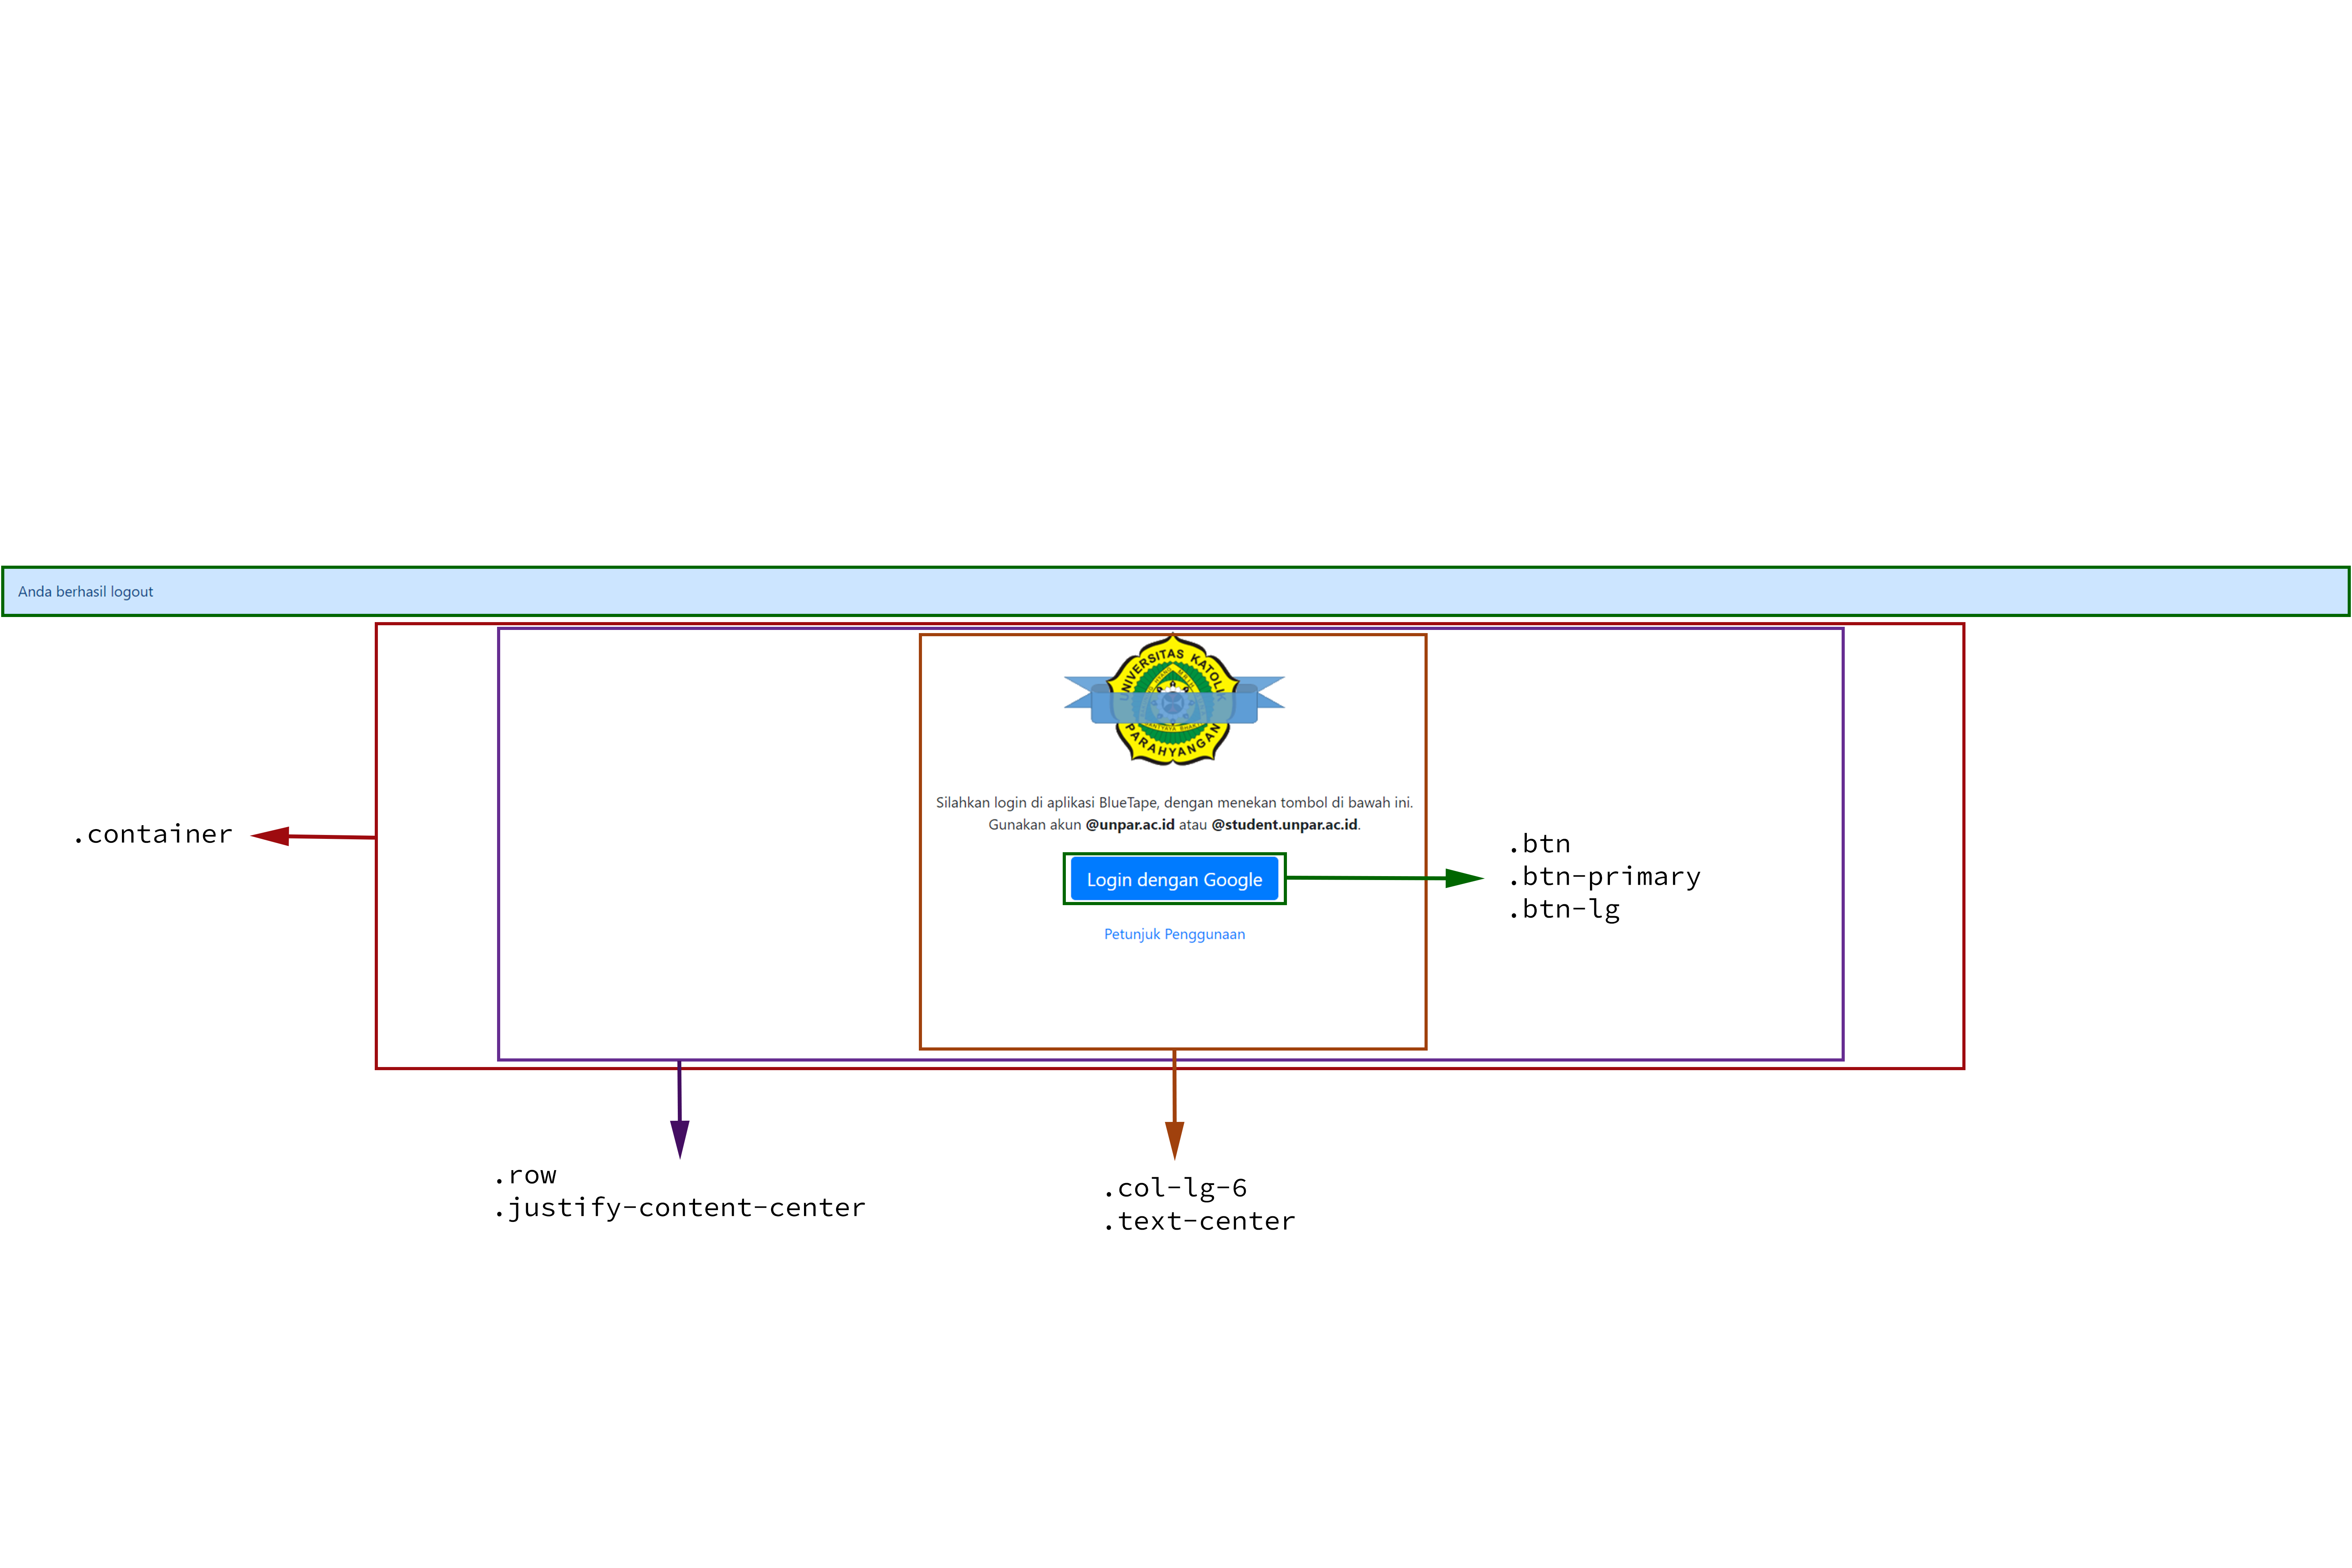
\includegraphics[trim=left botm right top, clip, width=\textwidth, height=\textheight,keepaspectratio]{bootstrap/konversi_tampilan_login.png}  
	\caption{Konversi Tampilan Login} 
\end{figure}
%Kode
\begin{lstlisting}[language=diff, caption=Kode untuk Halaman Login, label=Entri, basicstyle=\ttfamily, frame=single,
columns=fullflexible, keepspaces=true, breaklines=true]
--- C:\xampp\htdocs\BlueTape2\www\application\views\auth\login.php	
+++ C:\xampp\htdocs\BlueTape\www\application\views\auth\login.php	
@@ -4,26 +4,29 @@

-        <link rel="stylesheet" href="/public/css/foundation.css" />
-        <link rel="stylesheet" href="/public/css/app.css" />
+        <link rel="stylesheet" href="/public/lib/css/bootstrap.css" />
+        <link rel="stylesheet" href="/public/lib/css/bootstrap-grid.css" />
+        <link rel="stylesheet" href="/public/lib/css/bootstrap-reboot.css" />
+        <link rel="stylesheet" href="/public/lib/fontawesome/fontawesome.css" />


@@ Implementasi Komponen Grid @@
-        	<div class="row">
-        		<div class="large-6 large-centered columns centered">
+        <div class="container">
+        	<div class="row justify-content-center">
+        		<div class="col-lg-6">

@@ Implementasi Komponen Text @@
- 		<a href="<?= $authURL; ?>" class="button expand">Login dengan Google</a><br/><br/>
- 		<a class="text-center" href="https://github.com/ftisunpar/BlueTape/wiki/UserGuide" target="_blank">Petunjuk Penggunaan</a>
+ 		<a href="<?= $authURL; ?>" class="btn btn-primary btn-lg">Login dengan Google</a><br/><br/>
+ 		<a href="https://github.com/ftisunpar/BlueTape/wiki/UserGuide" target="_blank">Petunjuk Penggunaan</a>
\end{lstlisting}

\begin{lstlisting}[language=diff, caption=Kode untuk Notifikasi Login, label=Entri, basicstyle=\ttfamily, frame=single,
columns=fullflexible, keepspaces=true, breaklines=true]
--- C:\xampp\htdocs\BlueTape2\www\application\views\templates\flashmessage.php	2019-04-29 13:02:52.000000000 +0700
+++ C:\xampp\htdocs\BlueTape\www\application\views\templates\flashmessage.php	2020-03-06 09:56:06.000000000 +0700
@@ -1,10 +1,9 @@
<?php
defined('BASEPATH') OR exit('No direct script access allowed');
- ?><div class="row">
+ ?>
<?php if (isset($_SESSION['error'])): ?>
-        <div class="callout alert"><?= $_SESSION['error'] ?></div>
+        <div class="alert alert-danger" role="alert"><?= $_SESSION['error'] ?></div>
<?php endif; ?>
<?php if (isset($_SESSION['info'])): ?>
-        <div class="callout primary"><?= $_SESSION['info'] ?></div>
+        <div class="alert alert-primary" role="alert"><?= $_SESSION['info'] ?></div>
<?php endif; ?>
- </div>

\end{lstlisting}
\subsection{Menu Navigasi}
%Gambar
\begin{figure} [H]
	\centering  
	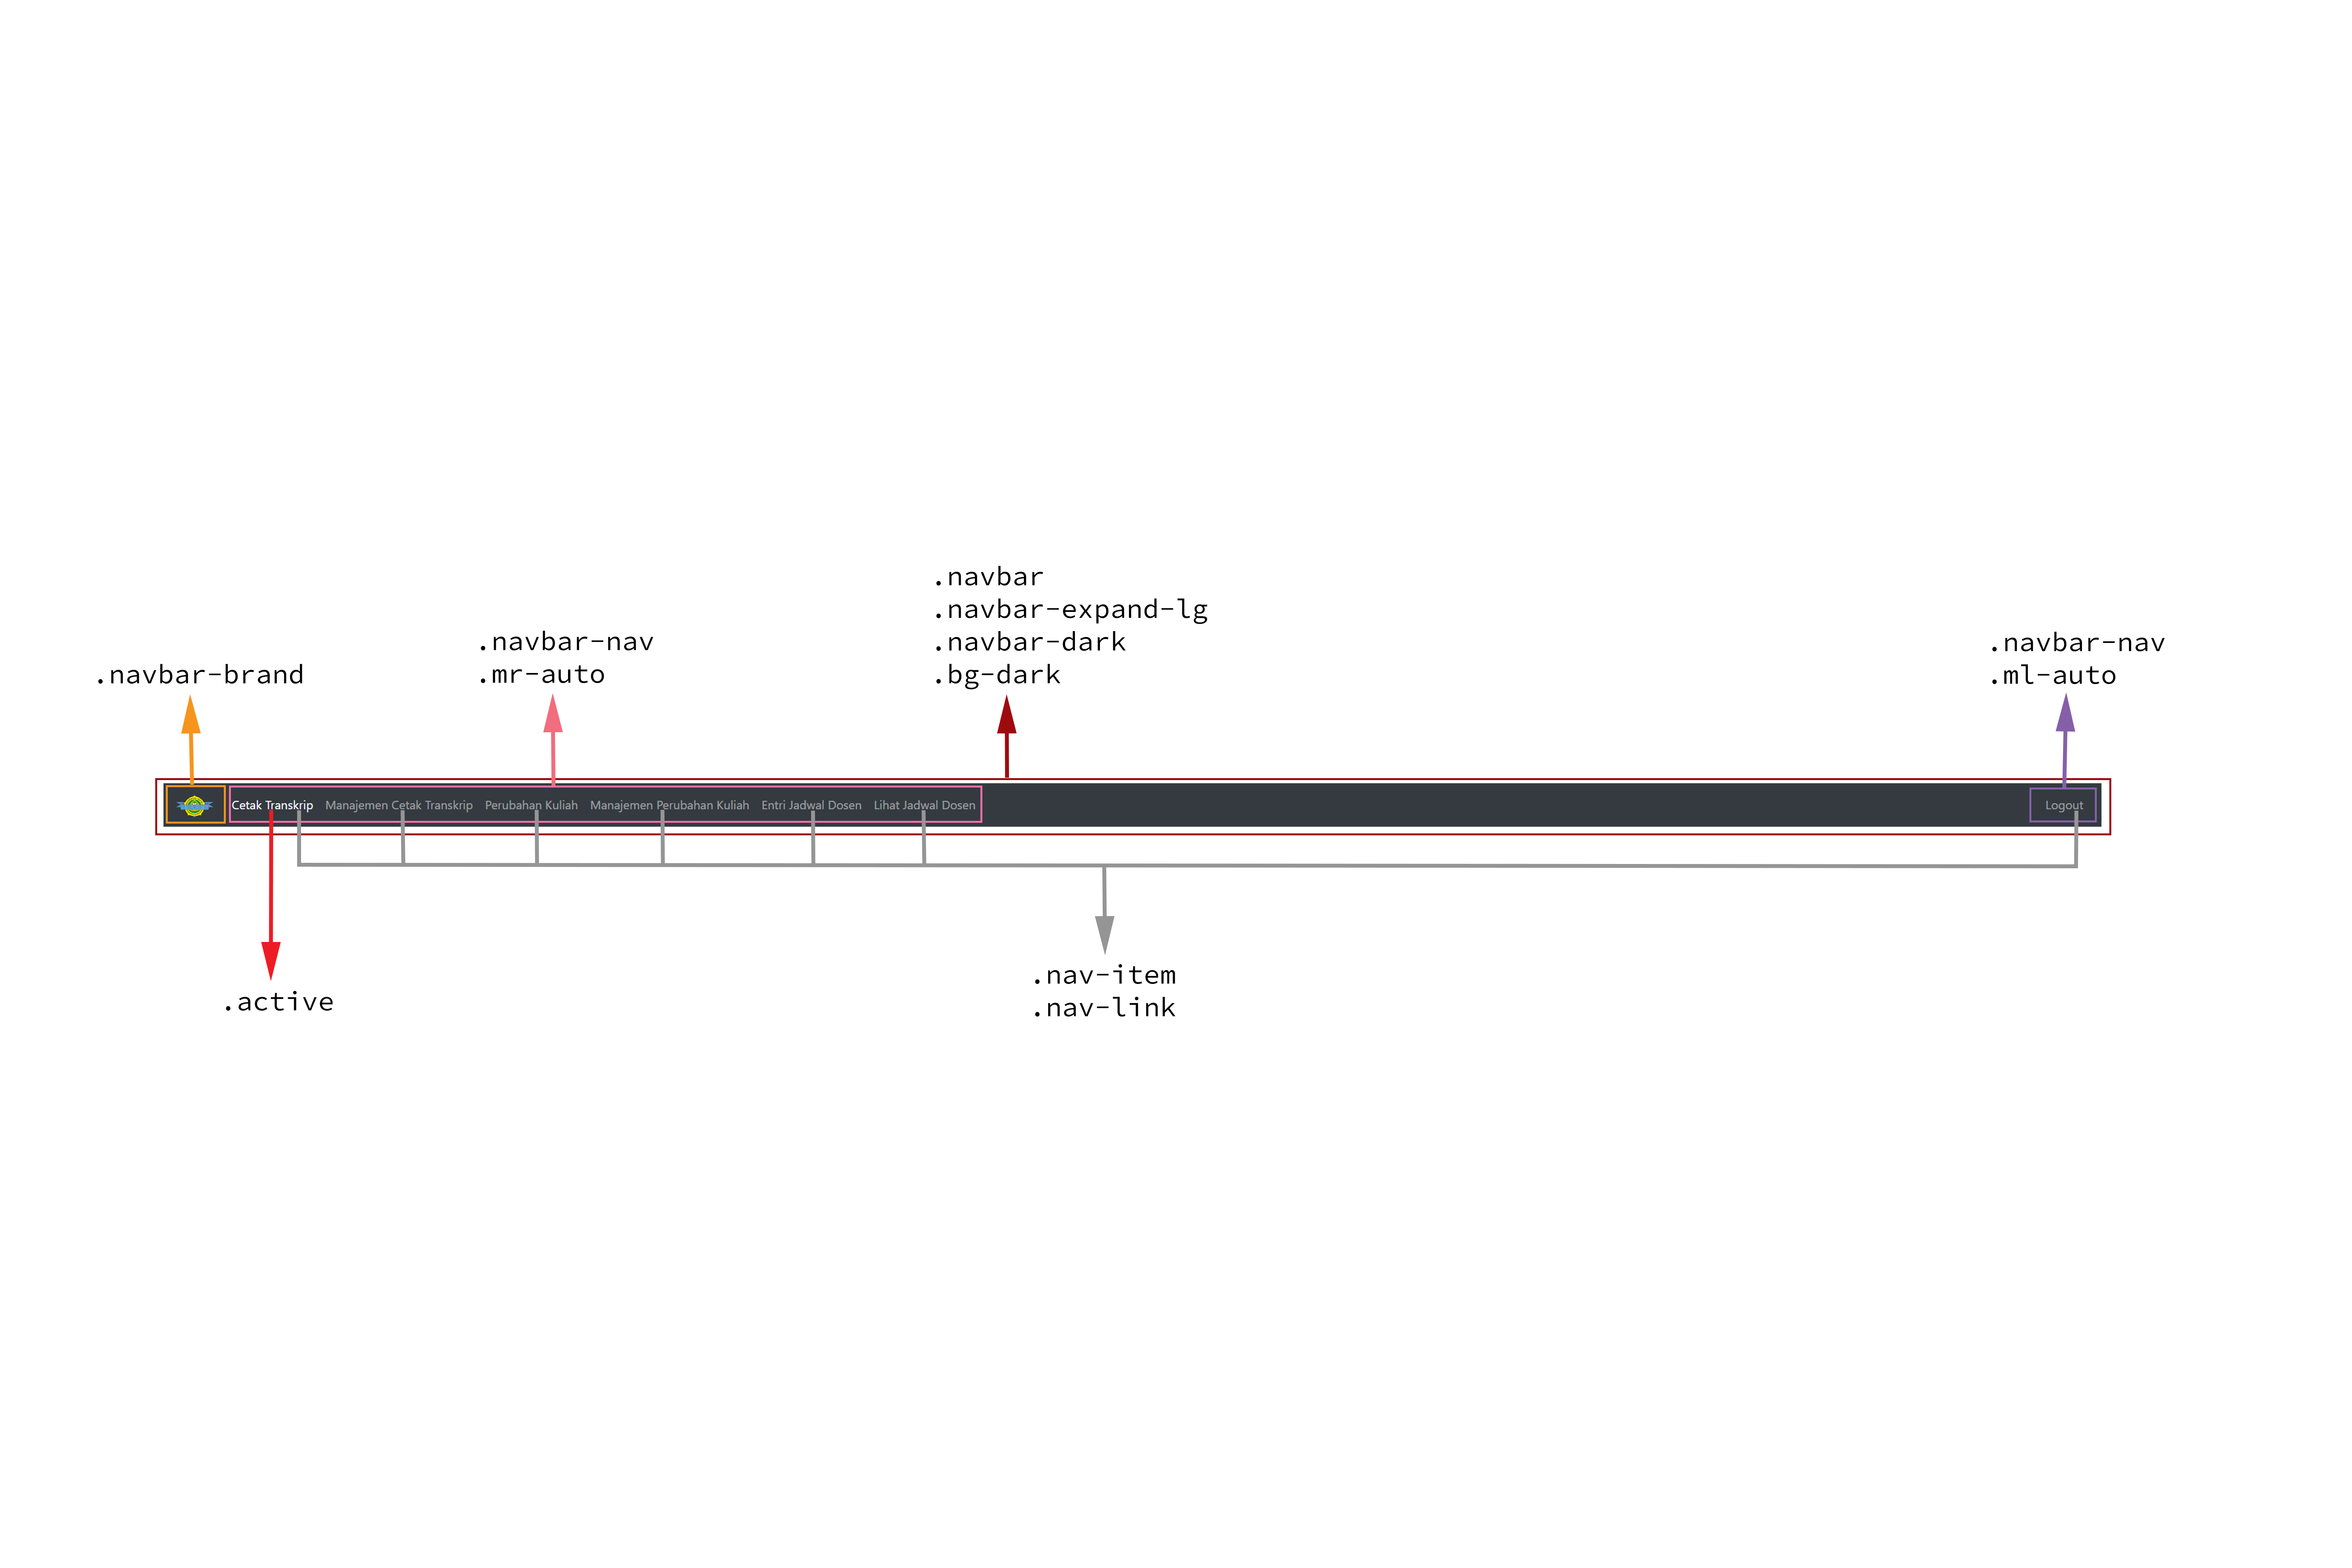
\includegraphics[width=\textwidth,height=\textheight,keepaspectratio]{bootstrap/konversi_navbar.png}  
	\caption{Konversi Tampilan Login} 
\end{figure}
\begin{figure} [H]
	\centering  
	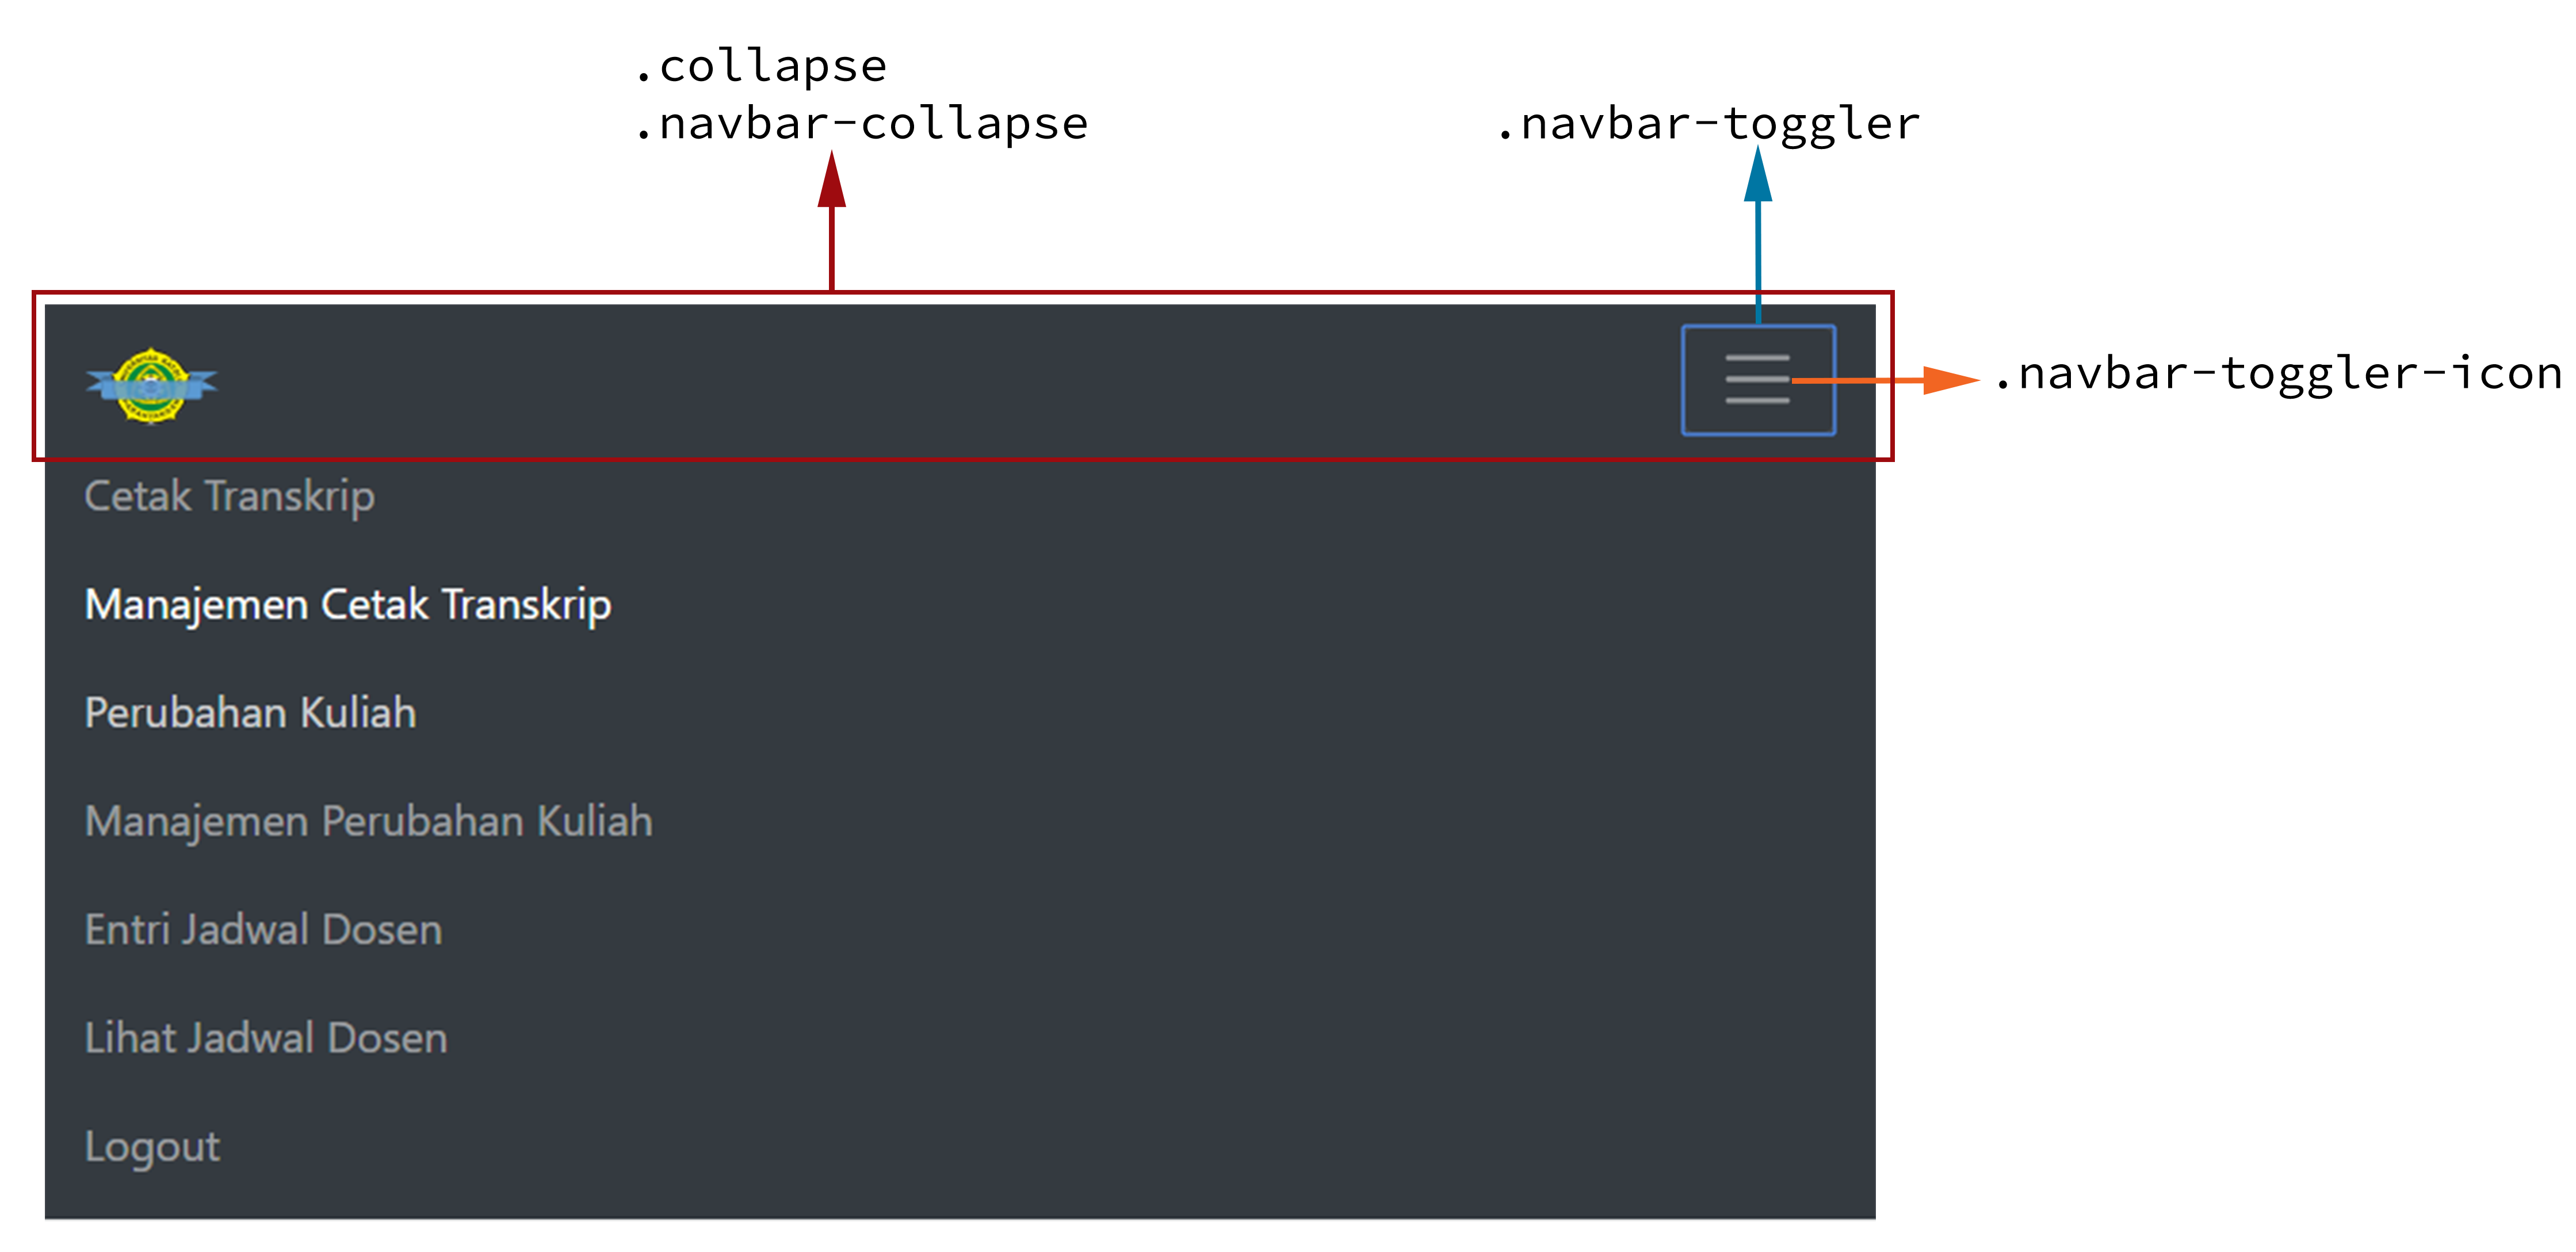
\includegraphics[width=\textwidth,height=\textheight,keepaspectratio]{bootstrap/konversi_small_navbar.png}  
	\caption{Konversi Tampilan Login} 
\end{figure}
%Kode
\begin{lstlisting}[language=diff, caption=Kode untuk Menu Navigasi, label=Entri, basicstyle=\ttfamily, frame=single,
columns=fullflexible, keepspaces=true, breaklines=true]
--- C:\xampp\htdocs\BlueTape2\www\application\views\templates\topbar_loggedin.php	2020-03-25 20:27:35.000000000 +0700
+++ C:\xampp\htdocs\BlueTape\www\application\views\templates\topbar_loggedin.php	2020-03-06 09:56:06.000000000 +0700

@@ Implementasi Komponen Navbar @@
- <div class="title-bar" data-responsive-toggle="navigation-menu" data-hide-for="medium">
- 	<button class="menu-icon" type="button" data-toggle></button>
- <div class="title-bar-title"><img src="/public/img/logo.png" class="textsized" alt="B"/></div>
- </div>
-
- <div class="top-bar" id="navigation-menu">
-  <div class="top-bar-left">
-    <ul class="menu" data-responsive-menu="dropdown">
-      <li class="menu-text"><img src="/public/img/logo.png" class="textsized" alt="B"/></li>
+ 		
+ 			
+ <nav class="navbar navbar-expand-lg navbar-dark bg-dark">
+   <a class="navbar-brand" href="#"><img src="/public/img/logo.png" width="50"/></a>
+ 	<button class="navbar-toggler" type="button" data-toggle="collapse" data-target="#navbarSupportedContent" aria-controls="navbarSupportedContent" aria-expanded="false" aria-label="Toggle navigation">
+ 		<span class="navbar-toggler-icon"></span>
+ 	</button>
+ 		
+ <div class="collapse navbar-collapse" id="navbarSupportedContent">
+ 	<ul class="navbar-nav mr-auto">

@@ Implementasi kelas .active @@
- <li<?= $module === $currentModule ? ' class="menu-active"' : '' ?>><a href="/<?= $module ?>"><?= $this->config->item('module-names')[$module] ?></a></li>
+ <li<?= $module == $currentModule ? ' class="nav-item active"' : ' class="nav-item "' ?>><a class="nav-link" href="/<?= $module ?>"><?= $this->config->item('module-names')[$module] ?></a></li>

@@ Implementasi Komponen Navbar @@
- </div>
- <div class="top-bar-right">
- 	<ul class="menu">
- 		<li><a href="/auth/logout">Logout</a></li>
+ 	<ul class="navbar-nav ml-auto">
+ 		<li class="nav-item">
+ 		    <a class="nav-link" href="/auth/logout">Logout</a>
+ 		</li>

\end{lstlisting}

\subsection{Halaman Cetak Transkrip Request}
\subsubsection{Halaman Utama}
\begin{figure} [H]
	\centering  
	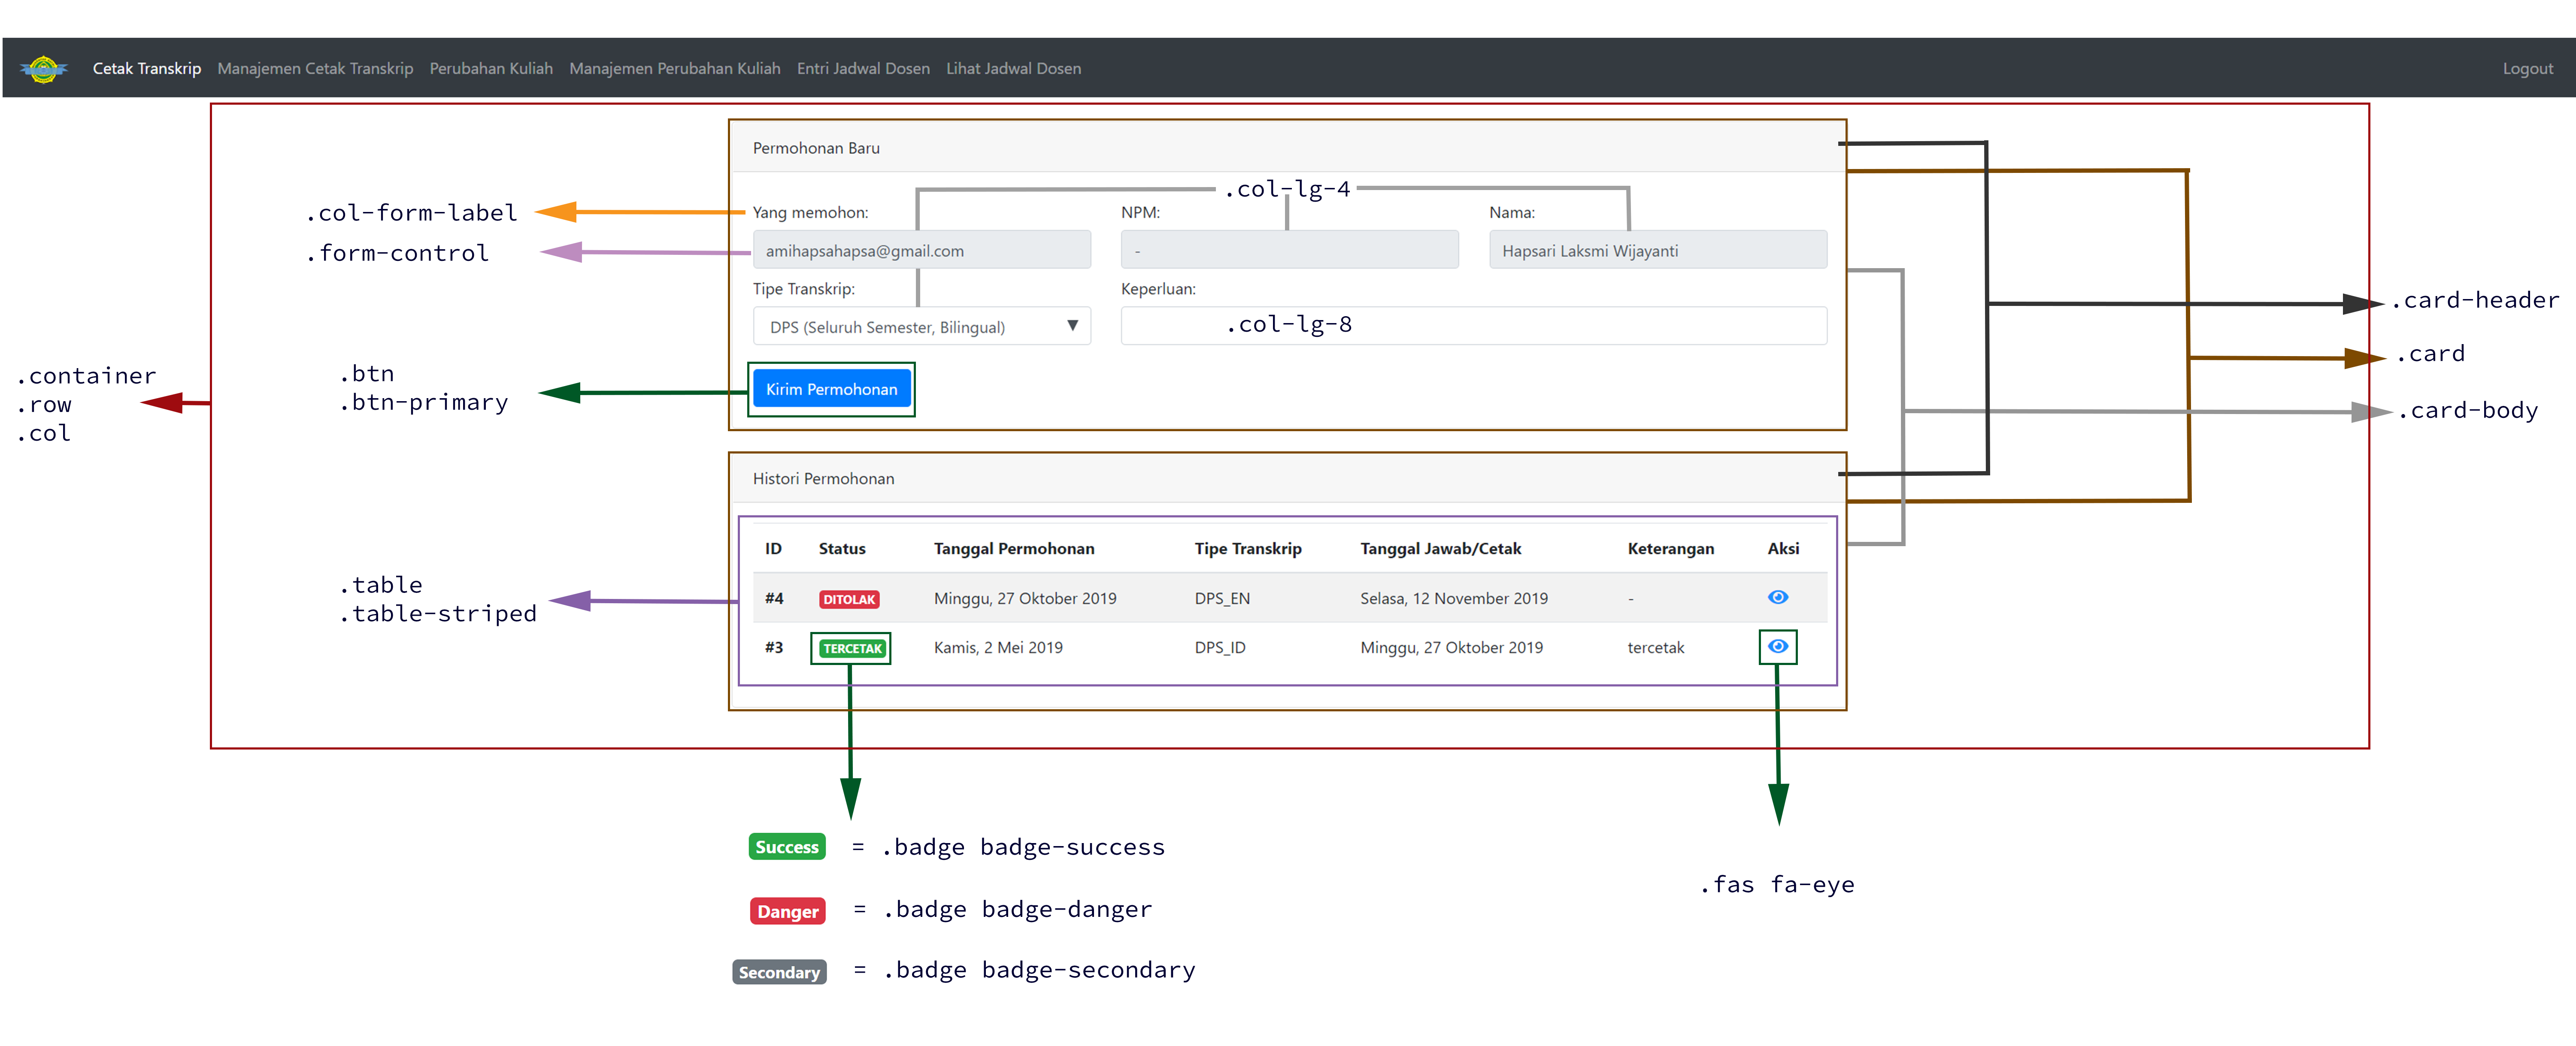
\includegraphics[width=\textwidth,height=\textheight,keepaspectratio]{bootstrap/konversi_tampilan_cetak_transkrip.png}  
	\caption{Konversi Halaman Cetak Transkrip Request} 
\end{figure}
\begin{lstlisting}[language=diff, caption=Kode untuk Halaman Cetak Transkrip Request, label=Entri, basicstyle=\ttfamily, frame=single,
columns=fullflexible, keepspaces=true, breaklines=true]
--- C:\xampp\htdocs\BlueTape2\www\application\views\TranskripRequest\main.php
+++ C:\xampp\htdocs\BlueTape\www\application\views\TranskripRequest\main.php

@@ Implementasi Komponen Grid dan Card @@
+ <div class="container">
<div class="row">
- <div class="medium-12 column">
-	<div class="callout">
-    		<h5>Permohonan Baru</h5>
+ <div class="col">
+    <div class="card">
+        <div class="card-header">
+            Permohonan Baru
+        </div>
+        <div class="card-body">

@@ Implementasi Komponen Form @@
- <div class="large-4 column">
-    <label>Yang memohon:
-        <input type="email" name="requestByEmail" value="<?= $requestByEmail ?>" readonly="readonly"/>
-    </label>
+ <div class="col-lg-4">
+    <label class="col-form-label">Yang memohon:</label>
+    <input class="form-control" type="email" name="requestByEmail" value="<?= $requestByEmail ?>" readonly/>

- <div class="large-4 column">
-    <label>NPM:
-        <input type="text" value="<?= $requestByNPM ?>" readonly="readonly"/>
-    </label>
+ <div class="col-lg-4">
+    <label class="col-form-label">NPM:</label>
+    <input class="form-control" type="text" value="<?= $requestByNPM ?>" readonly/>
</div>
- <div class="large-4 column">
-    <label>Nama:
-        <input type="text" name="requestByName" value="<?= $requestByName ?>" readonly="readonly"/>
-    </label>
+ <div class="col-lg-4">
+    <label class="col-form-label">Nama:</label>
+    <input class="form-control" type="text" name="requestByName" value="<?= $requestByName ?>" 

- <div class="large-4 column">
-    <label>Tipe Transkrip:
-        <select name="requestType">
+ <div class="col-lg-4">
+    <label class="col-form-label">Tipe Transkrip:</label>
+    <select class="form-control" name="requestType">

-    </label>
</div>
- <div class="large-8 column">
-    <label>Keperluan:
-        <input type="text" name="requestUsage" required/>
-    </label>
+ <div class="col-lg-8">
+    <label class="col-form-label">Keperluan:</label>
+    <input class="form-control" type="text" name="requestUsage" required/>

- <input type="submit" class="button" value="Kirim Permohonan">
+ <br>
+ <div class="row">
+ <div class="col-lg-12">
+    <input class="btn btn-primary" type="submit" class="button" value="Kirim Permohonan">
+ </div>
+ </div>

@@ Implementasi Komponen Card dan Tabel @@
- <div class="callout">
-    <h5>Histori Permohonan</h5>
-    <table class="stack">
+ </div>
+ <br>
+ <div class="card">
+ <div class="card-header">
+    Histori Permohonan
+ </div>
+ <div class="card-body">
+    <table class="table table-striped">

- <th>ID</th>
- <th>Status</th>
- <th>Tanggal Permohonan</th>
- <th>Tipe Transkrip</th>
- <th>Tanggal Jawab/Cetak</th>
- <th>Keterangan</th>
- <th>Aksi</th>
+ <th scope="col">ID</th>
+ <th scope="col">Status</th>
+ <th scope="col">Tanggal Permohonan</th>
+ <th scope="col">Tipe Transkrip</th>
+ <th scope="col">Tanggal Jawab/Cetak</th>
+ <th scope="col">Keterangan</th>
+ <th scope="col">Aksi</th>

- <td>#<?= $request->id ?></td>
- <td><span class="<?= $request->labelClass ?> label"><?= $request->status ?></span></td>
+ <th>#<?= $request->id ?></th>
+ <td><span class="badge badge-<?= $request->labelClass ?>"><?= $request->status ?></span></td>
\end{lstlisting}


\subsubsection{Modal}
\begin{figure} [H]
	\centering  
	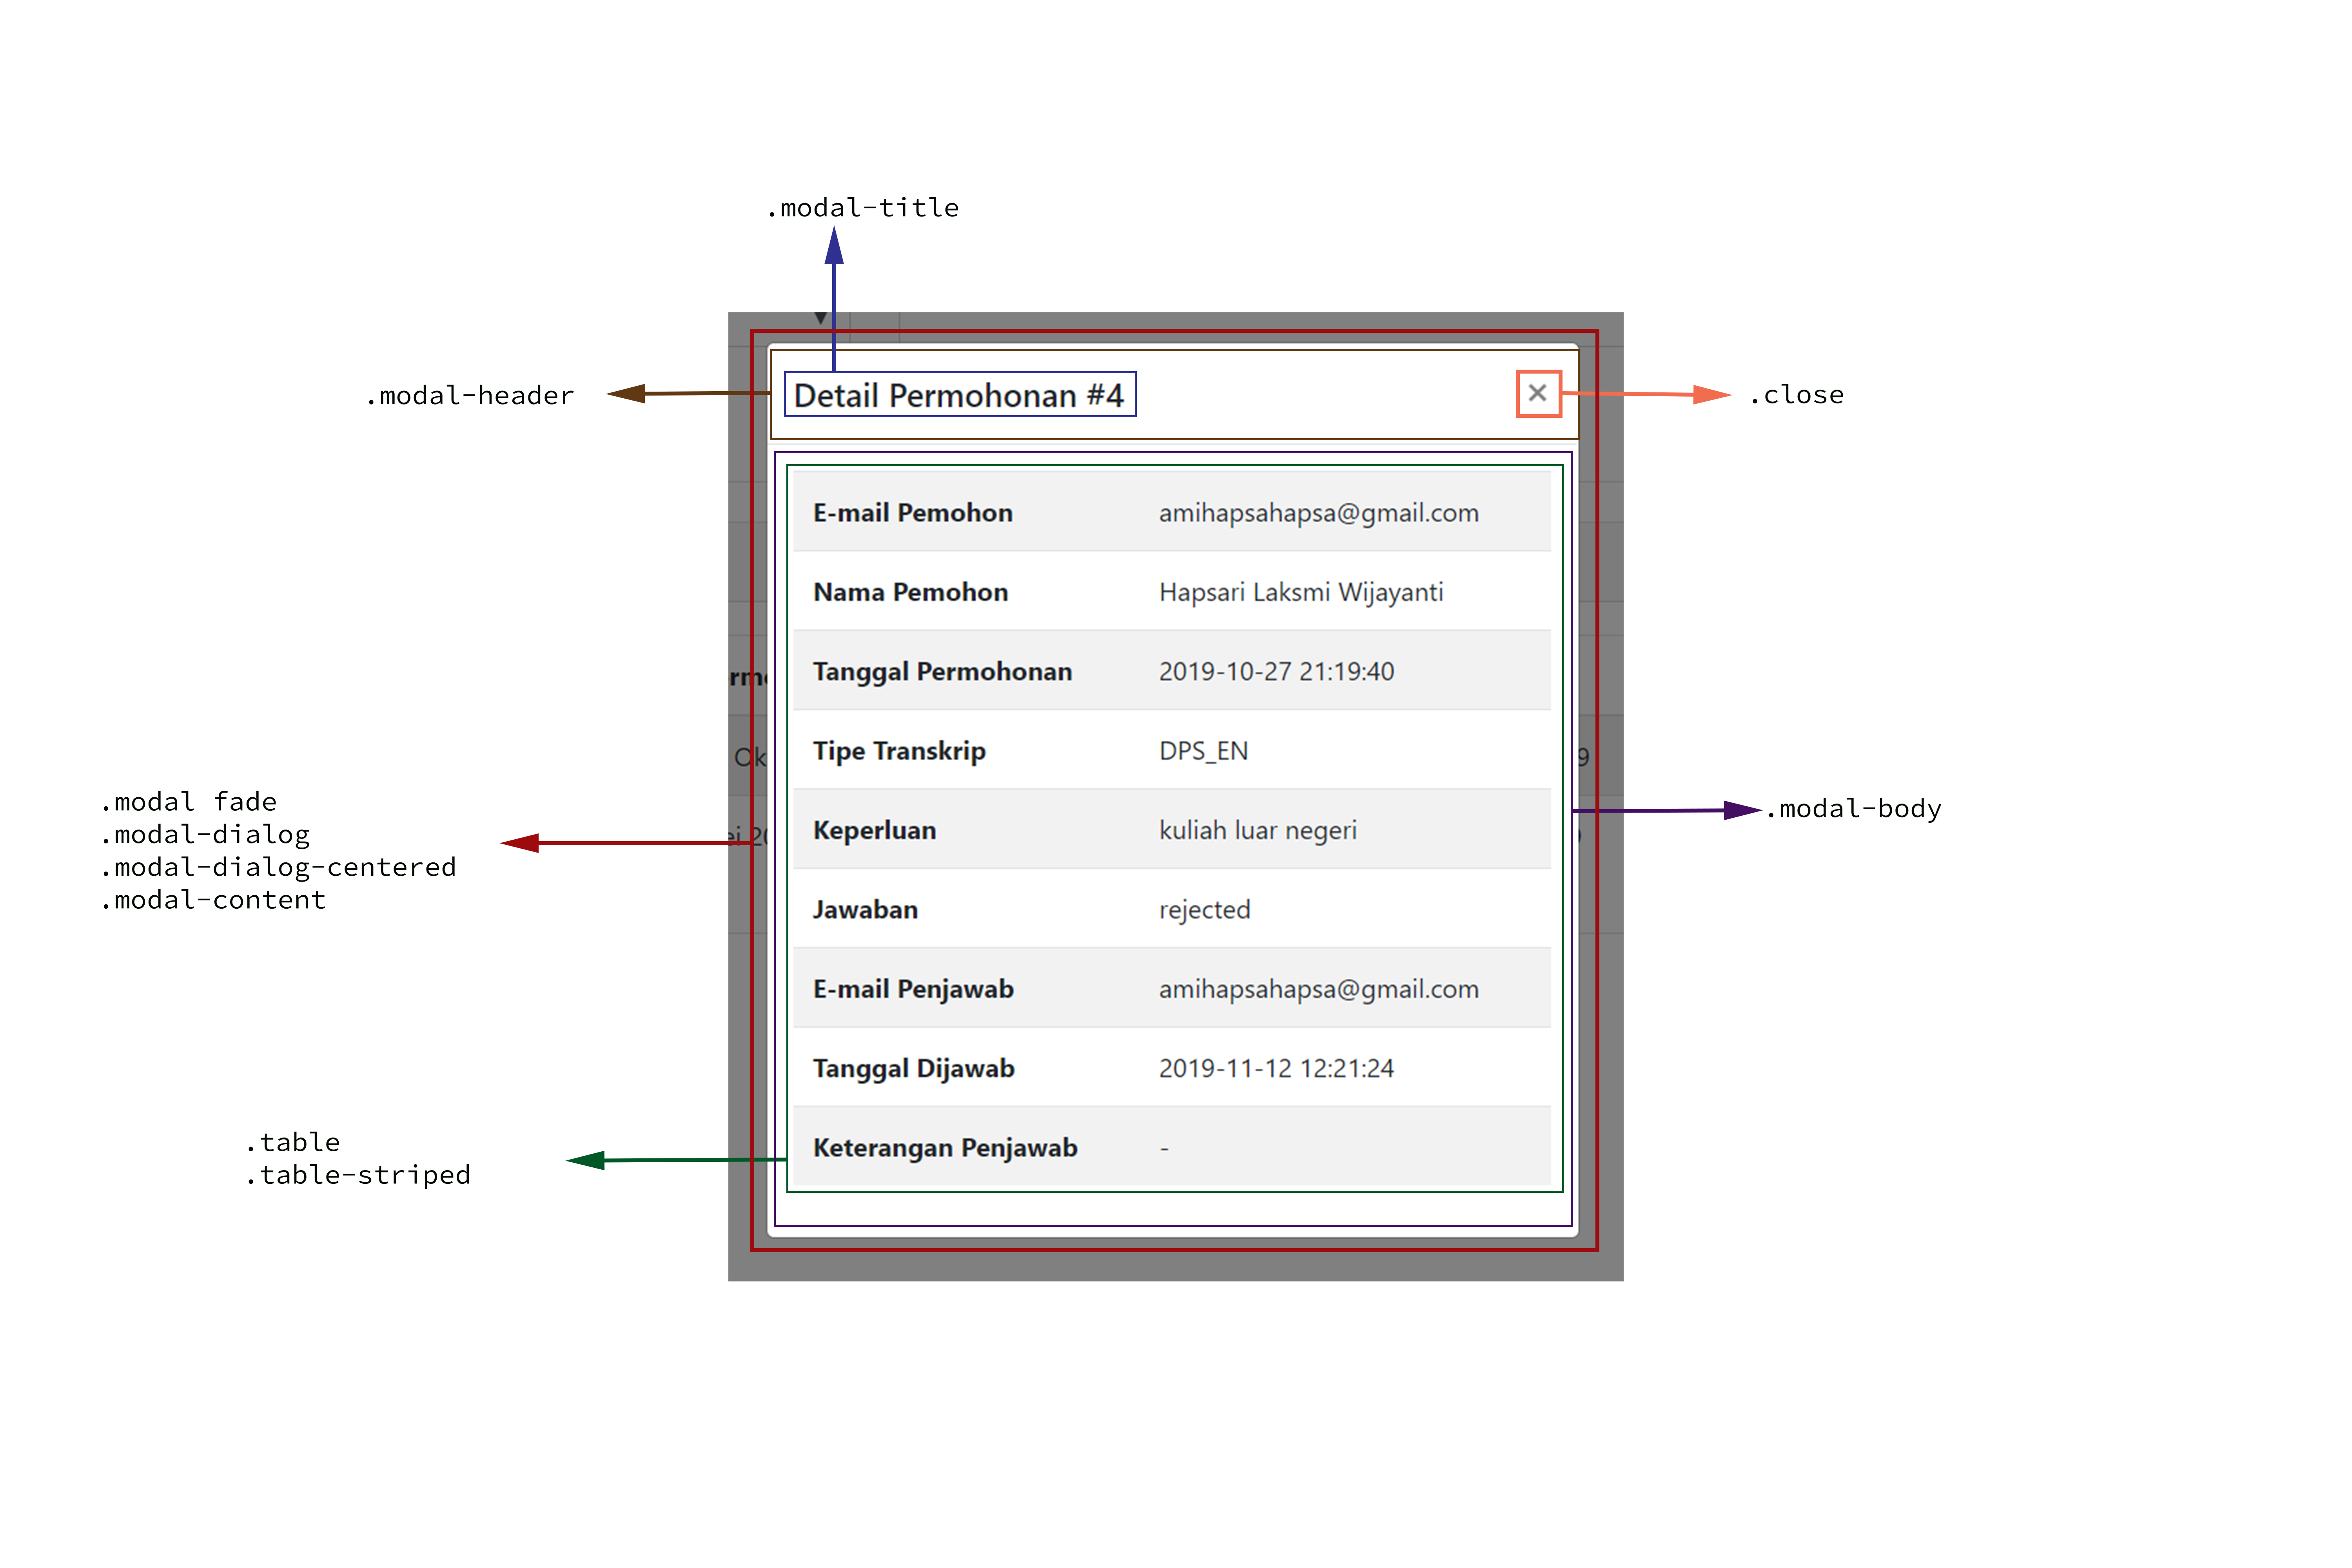
\includegraphics[width=\textwidth,height=\textheight,keepaspectratio]{bootstrap/konversi_modal_lihat_cetak_transkrip.png}  
	\caption{Konversi Halaman Cetak Transkrip Request} 
\end{figure}
\begin{lstlisting}[language=diff, caption=Kode untuk Modal Cetak Transkrip Manage, label=Entri, basicstyle=\ttfamily, frame=single,
columns=fullflexible, keepspaces=true, breaklines=true]
@@ Implementasi Komponen Modal @@
-    <div class="reveal" id="detail<?= $request->id ?>" data-reveal>
+ <!-- Button trigger modal -->
+ <a data-toggle="modal" data-target="#lihatModal<?= $request->id ?>" id="detail<?= $request->id ?>">
+ <i class="fas fa-eye"></i>
+ </a>
-        <h5>Detail Permohonan #<?= $request->id ?></h5>
-        <table class="stack">
+<!-- Modal -->
+<div class="modal fade" id="lihatModal<?= $request->id ?>" tabindex="-1" role="dialog" aria-labelledby="exampleModalCenterTitle" aria-hidden="true">
+ <div class="modal-dialog modal-dialog-centered" role="document">
+    <div class="modal-content">
+        <div class="modal-header">
+            <h5 class="modal-title" id="exampleModalLongTitle">Detail Permohonan #<?= $request->id ?></h5>
+            <button type="button" class="close" data-dismiss="modal" aria-label="Close">
+                <span aria-hidden="true">&times;</span>
+            </button>
+        </div>
+        <div class="modal-body">
+            <table class="table ">

@@ Implementasi Komponen Tabel@@
- <th>Jawaban</th>
+ <th scope="col">Jawaban</th>
\end{lstlisting}

\subsection{Halaman Cetak Transkrip Manage}
\subsubsection{Halaman Utama}
\begin{figure} [H]
	\centering  
	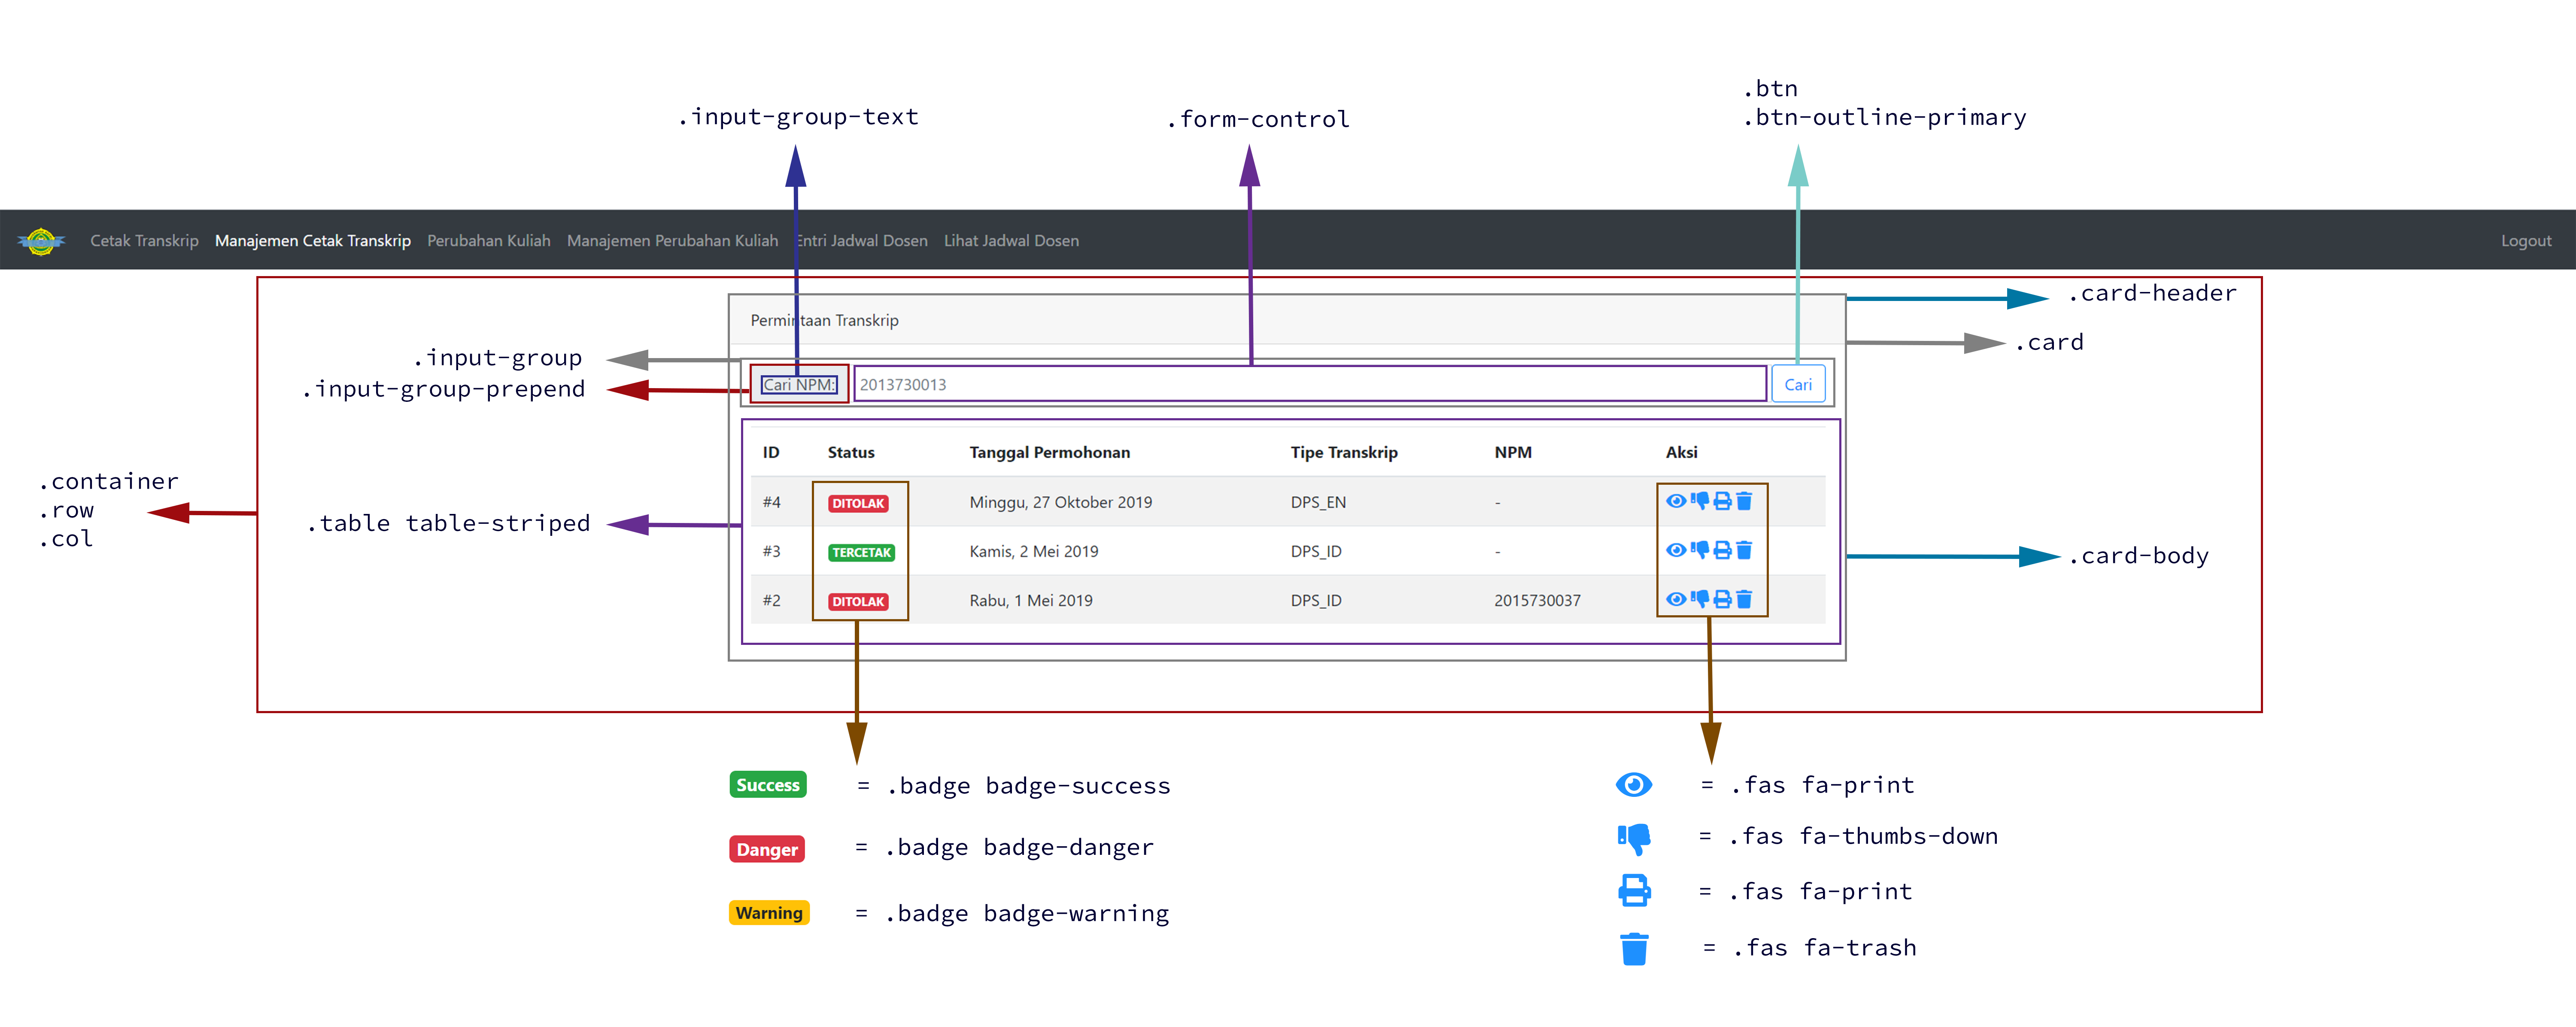
\includegraphics[width=\textwidth,height=\textheight,keepaspectratio]{bootstrap/konversi_tampilan_manajemen_cetak_transkrip.png}  
	\caption{Konversi Halaman Cetak Transkrip Manage} 
\end{figure}
\begin{lstlisting}[language=diff, caption=Kode untuk Halaman Cetak Transkrip Manage, label=Entri, basicstyle=\ttfamily, frame=single,
columns=fullflexible, keepspaces=true, breaklines=true]
--- C:\xampp\htdocs\BlueTape2\www\application\views\TranskripManage\main.php
+++ C:\xampp\htdocs\BlueTape\www\application\views\TranskripManage\main.php

@@ Implementasi Komponen Grid dan Card @@
- <div class="row">
-    <div class="callout">
-        <h5>Permintaan Transkrip</h5>
+ <div class="container">
+        <div class="card">
+            <div class="card-header">
+                Permintaan Transkrip
+            </div>
+            <div class="card-body">

@@ Implementasi Komponen Input Group @@ 
- <div class="input-group">
- <span class="input-group-label">Cari NPM:</span>
+ <div class="input-group mb-3">
+ <div class="input-group-prepend">
+    <span class="input-group-text">Cari NPM:</span>
+ </div>

- <input name="npm" class="input-group-field" type="text" placeholder="2013730013" maxlength="10" minlength="10"<?= $npmQuery === NULL ? '' : " value='$npmQuery'" ?>/>
- <div class="input-group-button">
-    <input class="button" type="submit" value="Cari"/>
+ <input name="npm" class="form-control" type="text" placeholder="2013730013" maxlength="10" minlength="10"<?= $npmQuery === NULL ? '' : " value='$npmQuery'" ?>/>
+ <div class="input-group-append">
+    <input class="btn btn-primary" type="submit" value="Cari"/>

@@ Implementasi Komponen Tabel @@ 
- <table class="stack">
+ <br>
+ <table class="table table-striped">

- <th>ID</th>
- <th>Status</th>
- <th>Tanggal Permohonan</th>
- <th>Tipe Transkrip</th>
- <th>NPM</th>
- <th>Aksi</th>
+ <th scope="col">ID</th>
+ <th scope="col">Status</th>
+ <th scope="col">Tanggal Permohonan</th>
+ <th scope="col">Tipe Transkrip</th>
+ <th scope="col">NPM</th>
+ <th scope="col">Aksi</th>

- <td><span class="<?= $request->labelClass ?> label"><?= $request->status ?></span></td>
+ <td><span class="badge badge-<?= $request->labelClass ?>"><?= $request->status ?></span></td>
\end{lstlisting}

\subsubsection{Modal}
\begin{figure}	
	\centering
	\begin{subfigure}[t]{3in}
		\centering  
		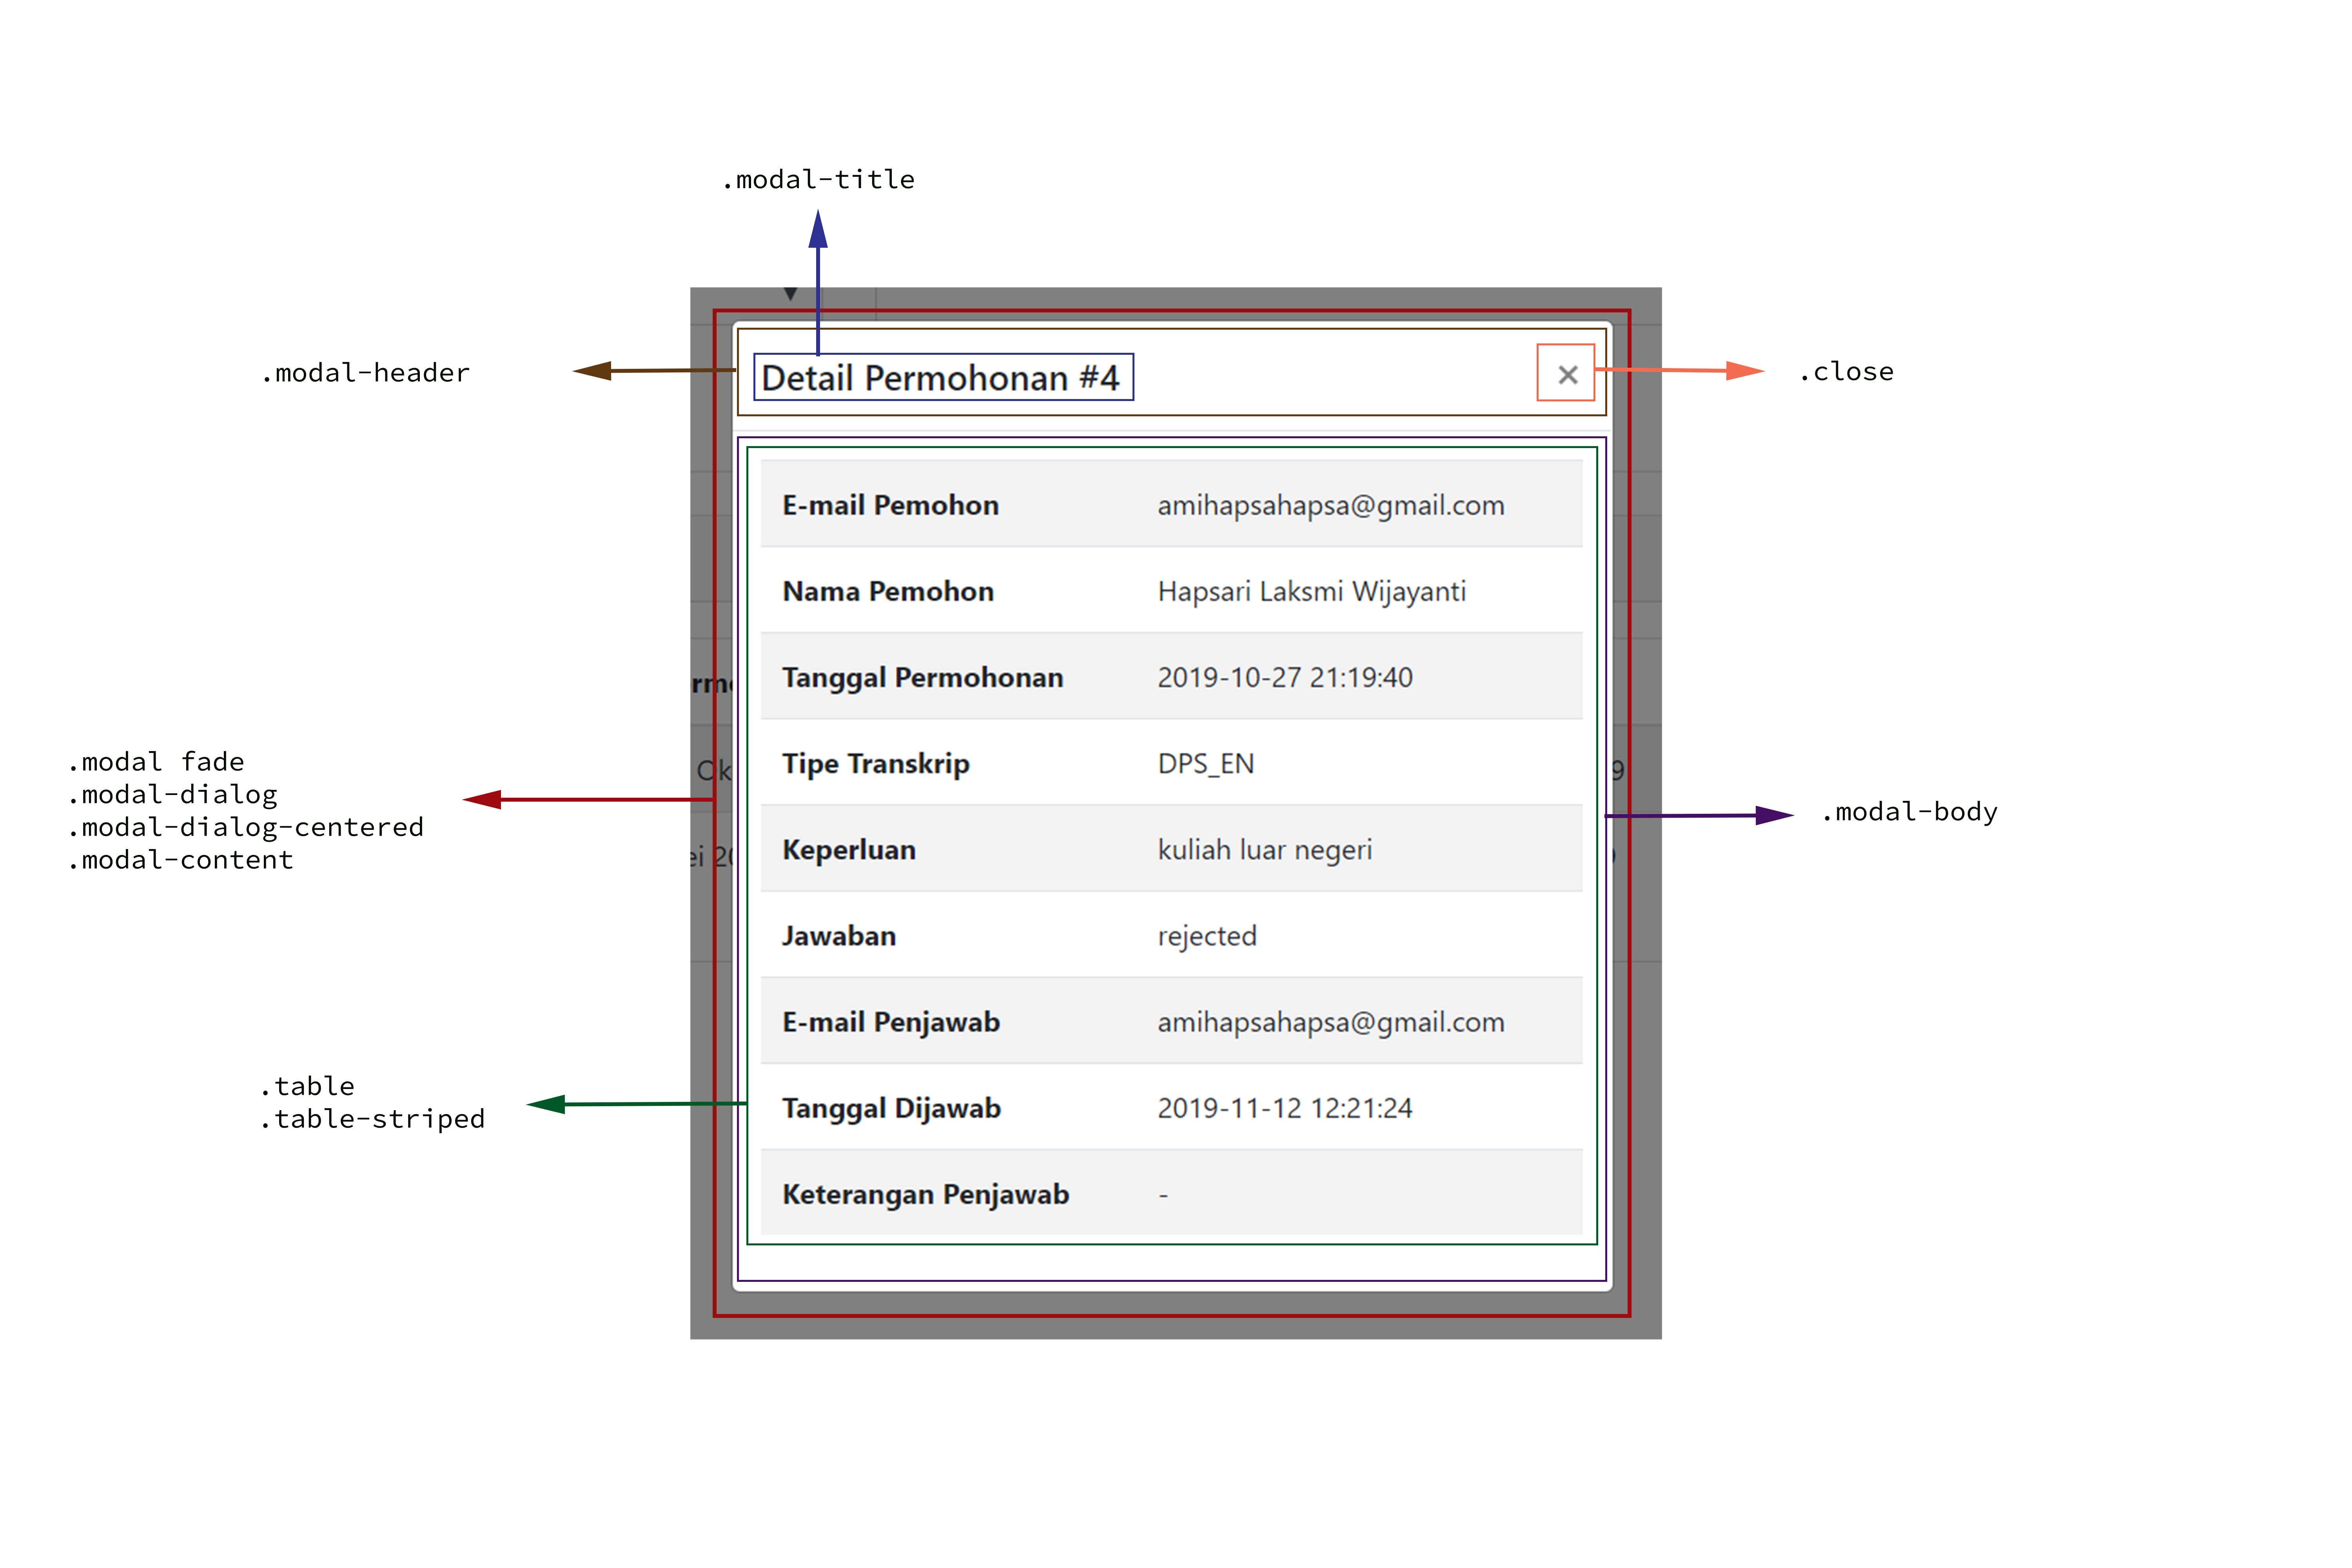
\includegraphics[width=\textwidth,height=\textheight,keepaspectratio]{bootstrap/konversi_modal_lihat_manajemen_cetak_transkrip.png}
		\caption{Konversi Modal Lihat} 
	\end{subfigure}
	\quad
	\begin{subfigure}[t]{3in}
		\centering  
		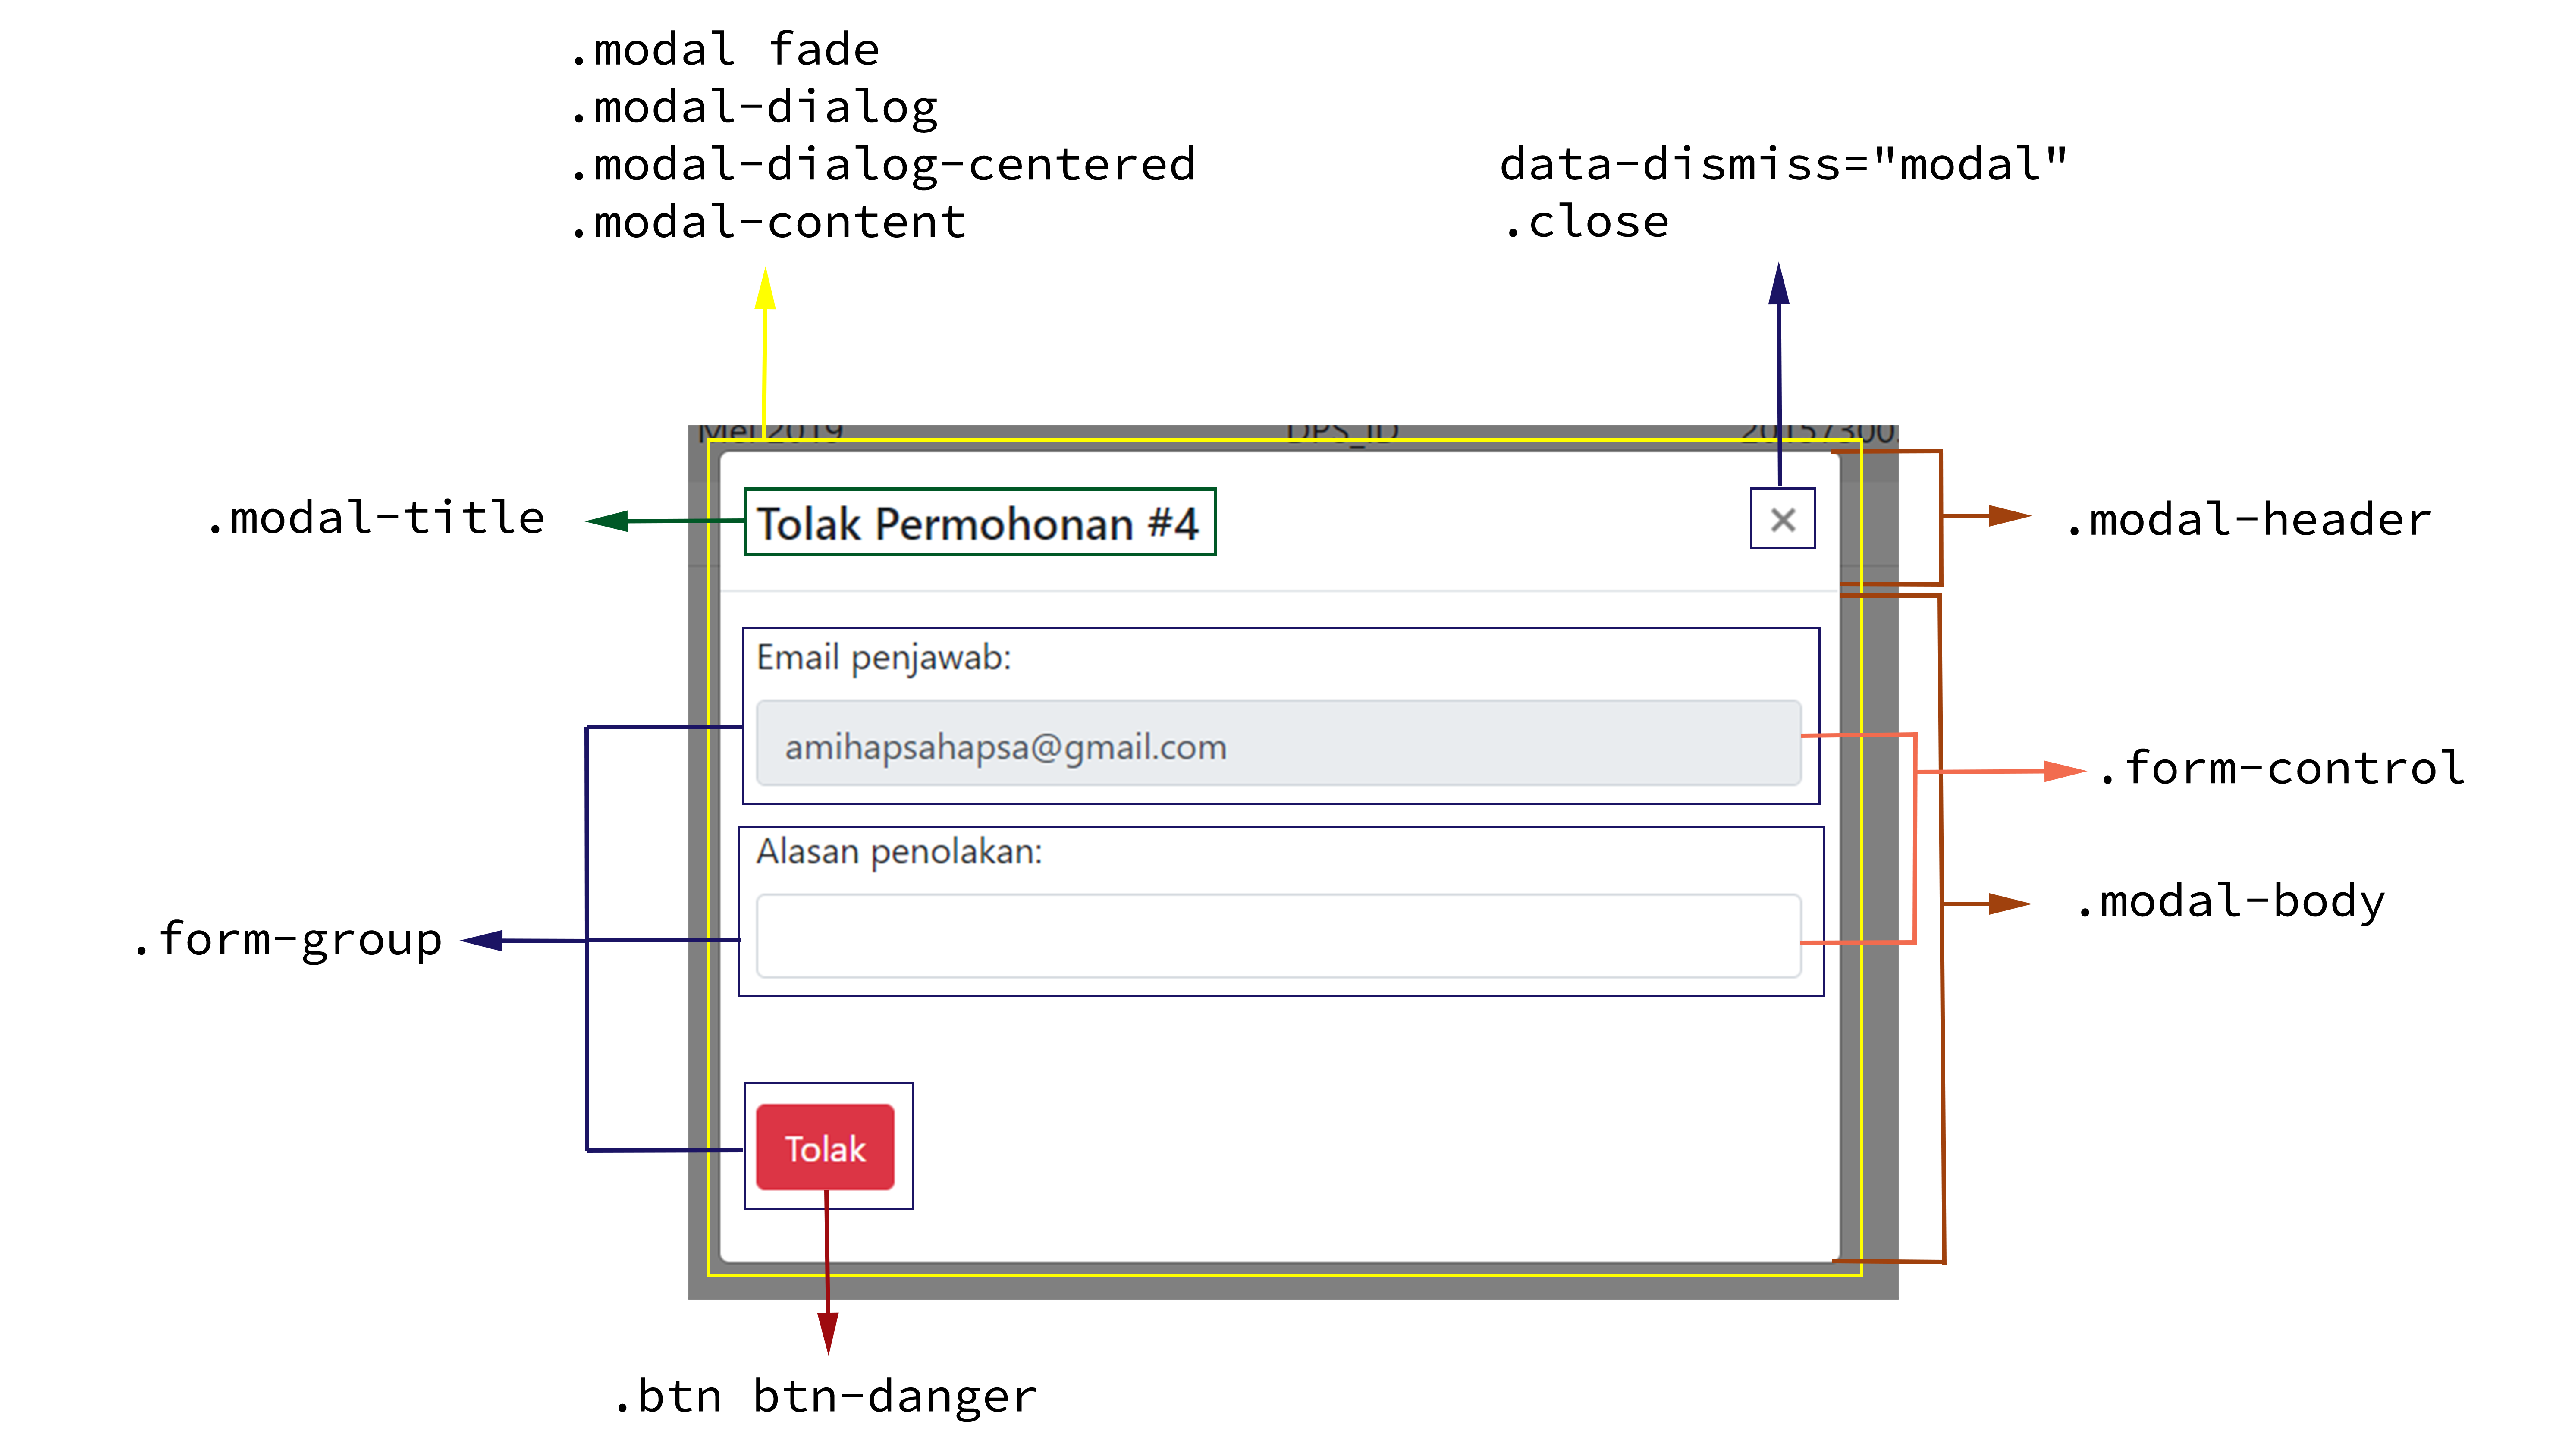
\includegraphics[width=\textwidth,height=\textheight,keepaspectratio]{bootstrap/konversi_modal_dislike_manajemen_cetak-tanskrip.png}
		\caption{Konversi Modal Tolak} 
	\end{subfigure}
\end{figure}
\begin{figure}	
	\centering
	\begin{subfigure}[t]{3in}
		\centering  
		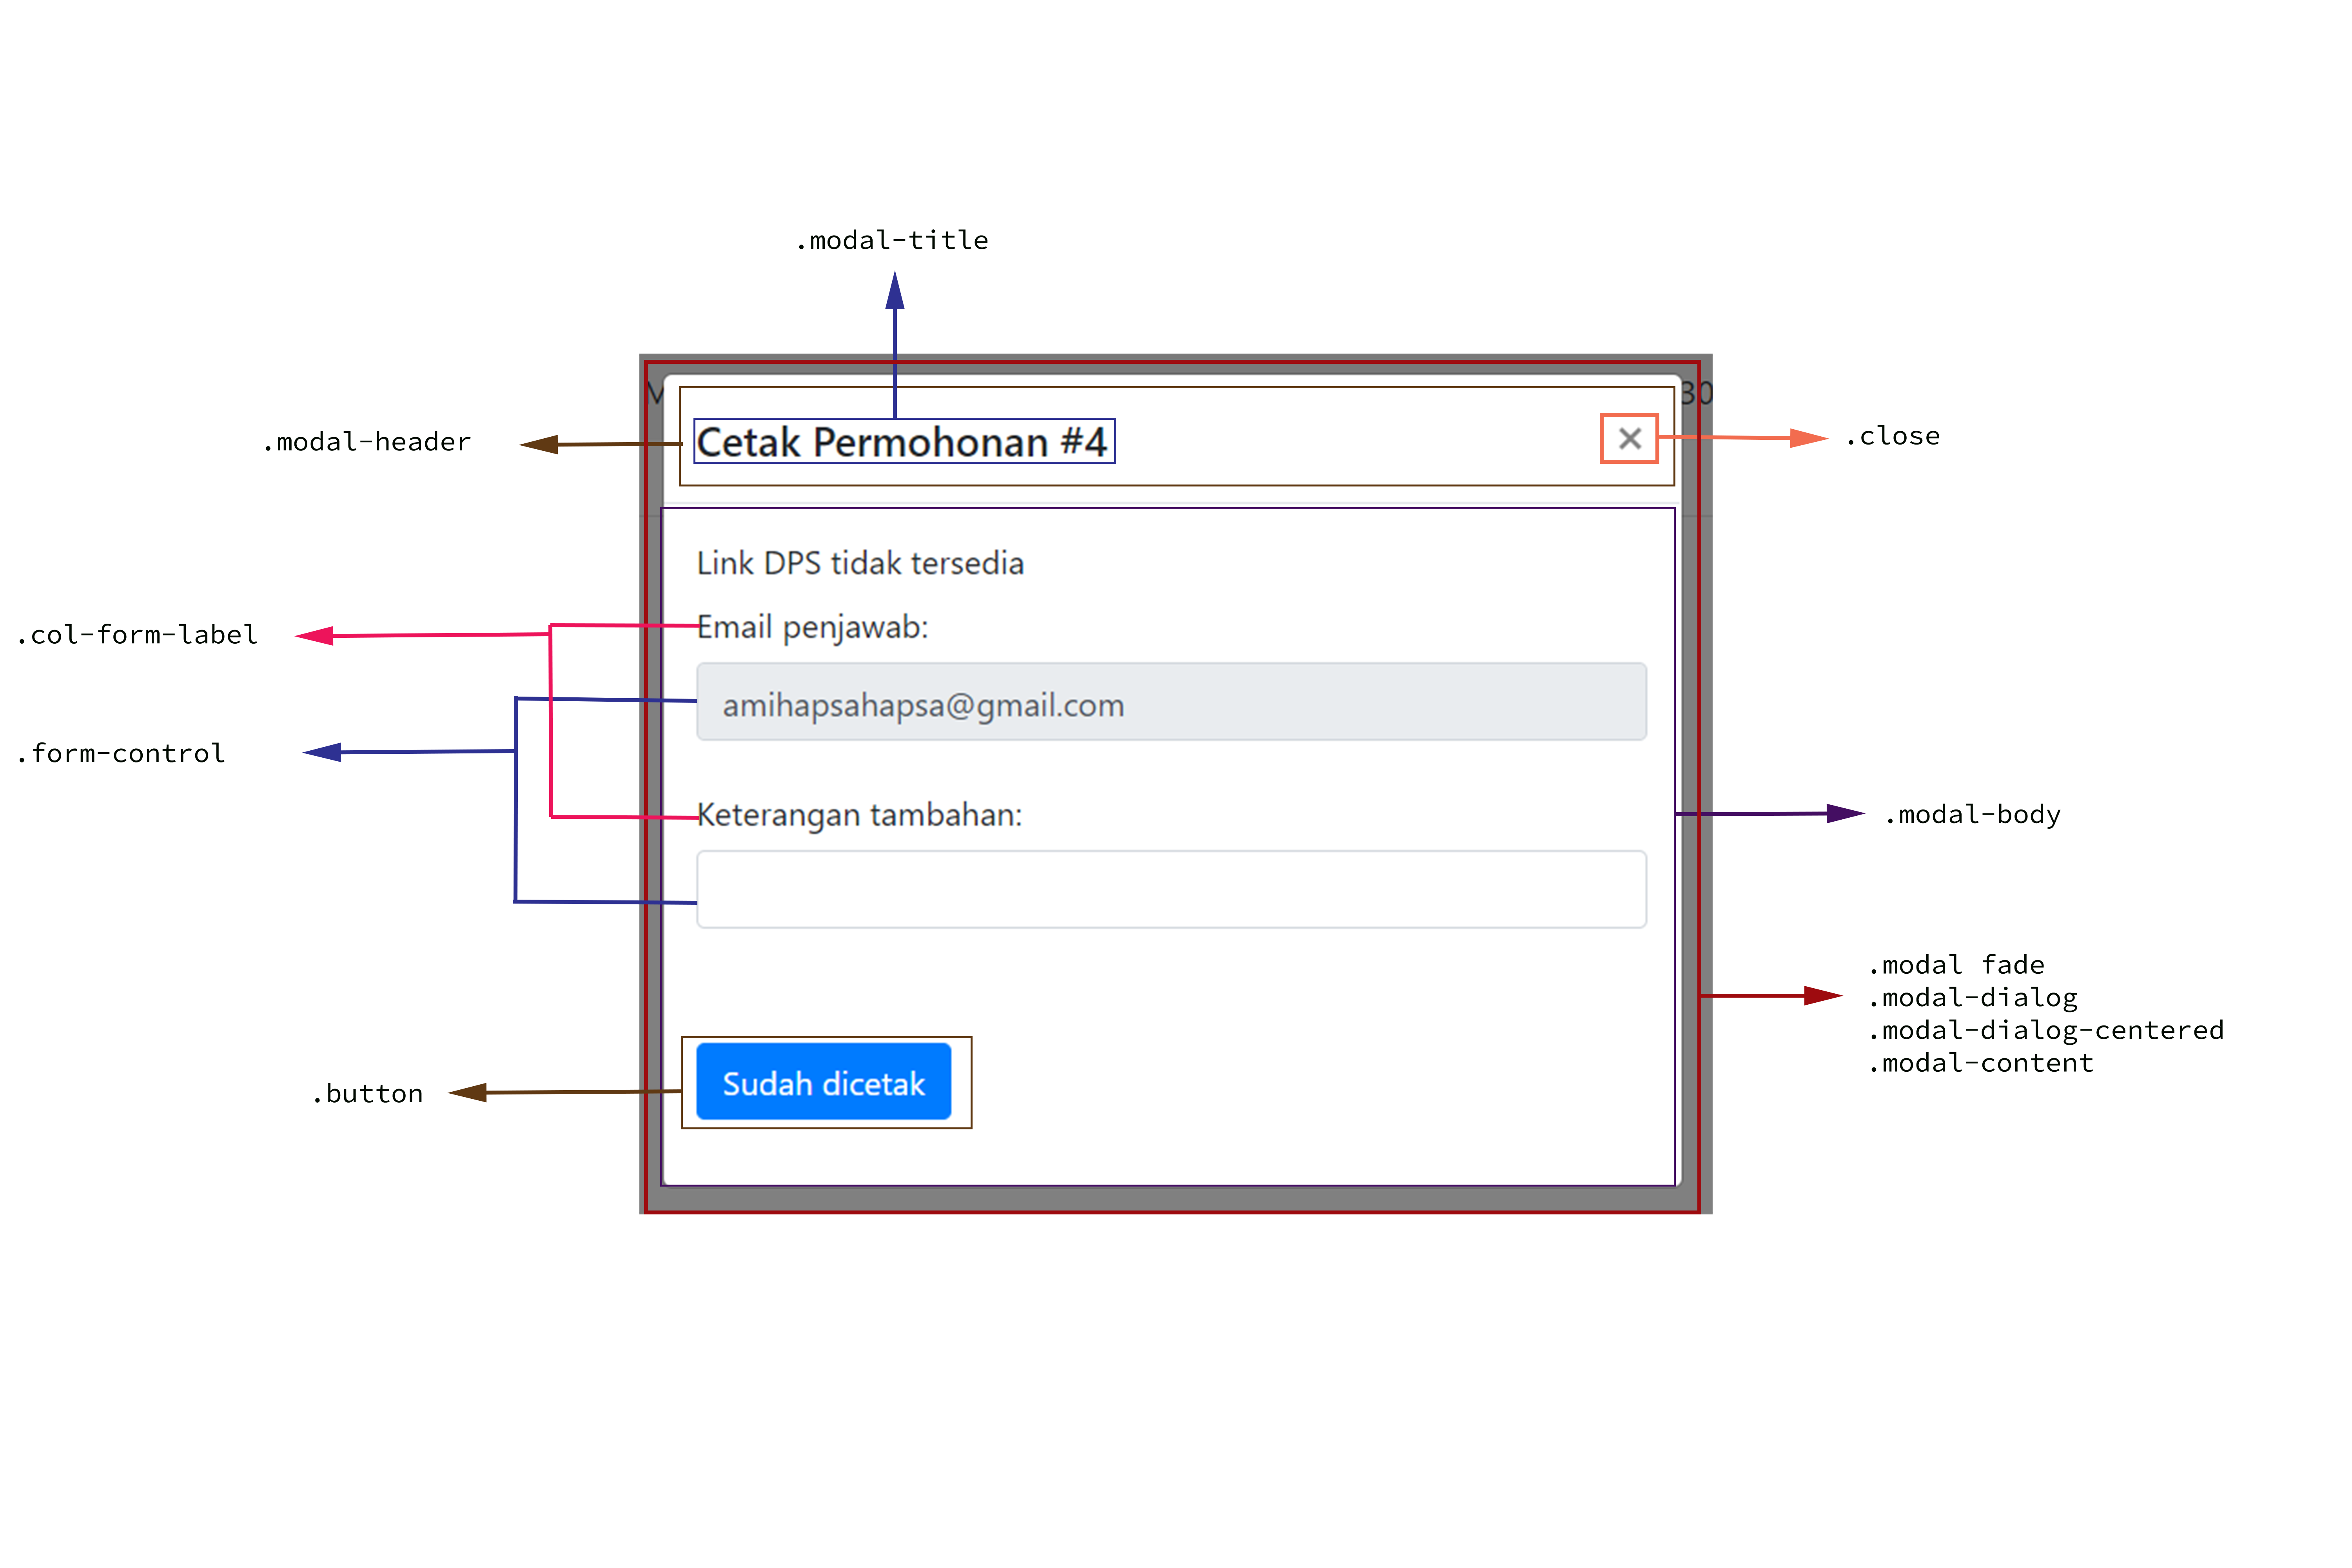
\includegraphics[width=\textwidth,height=\textheight,keepaspectratio]{bootstrap/konversi_modal_print_manajemen_cetak_transkrip.png}
		\caption{Konversi Modal Print} 
	\end{subfigure}
	\quad
	\begin{subfigure}[t]{3in}
		\centering  
		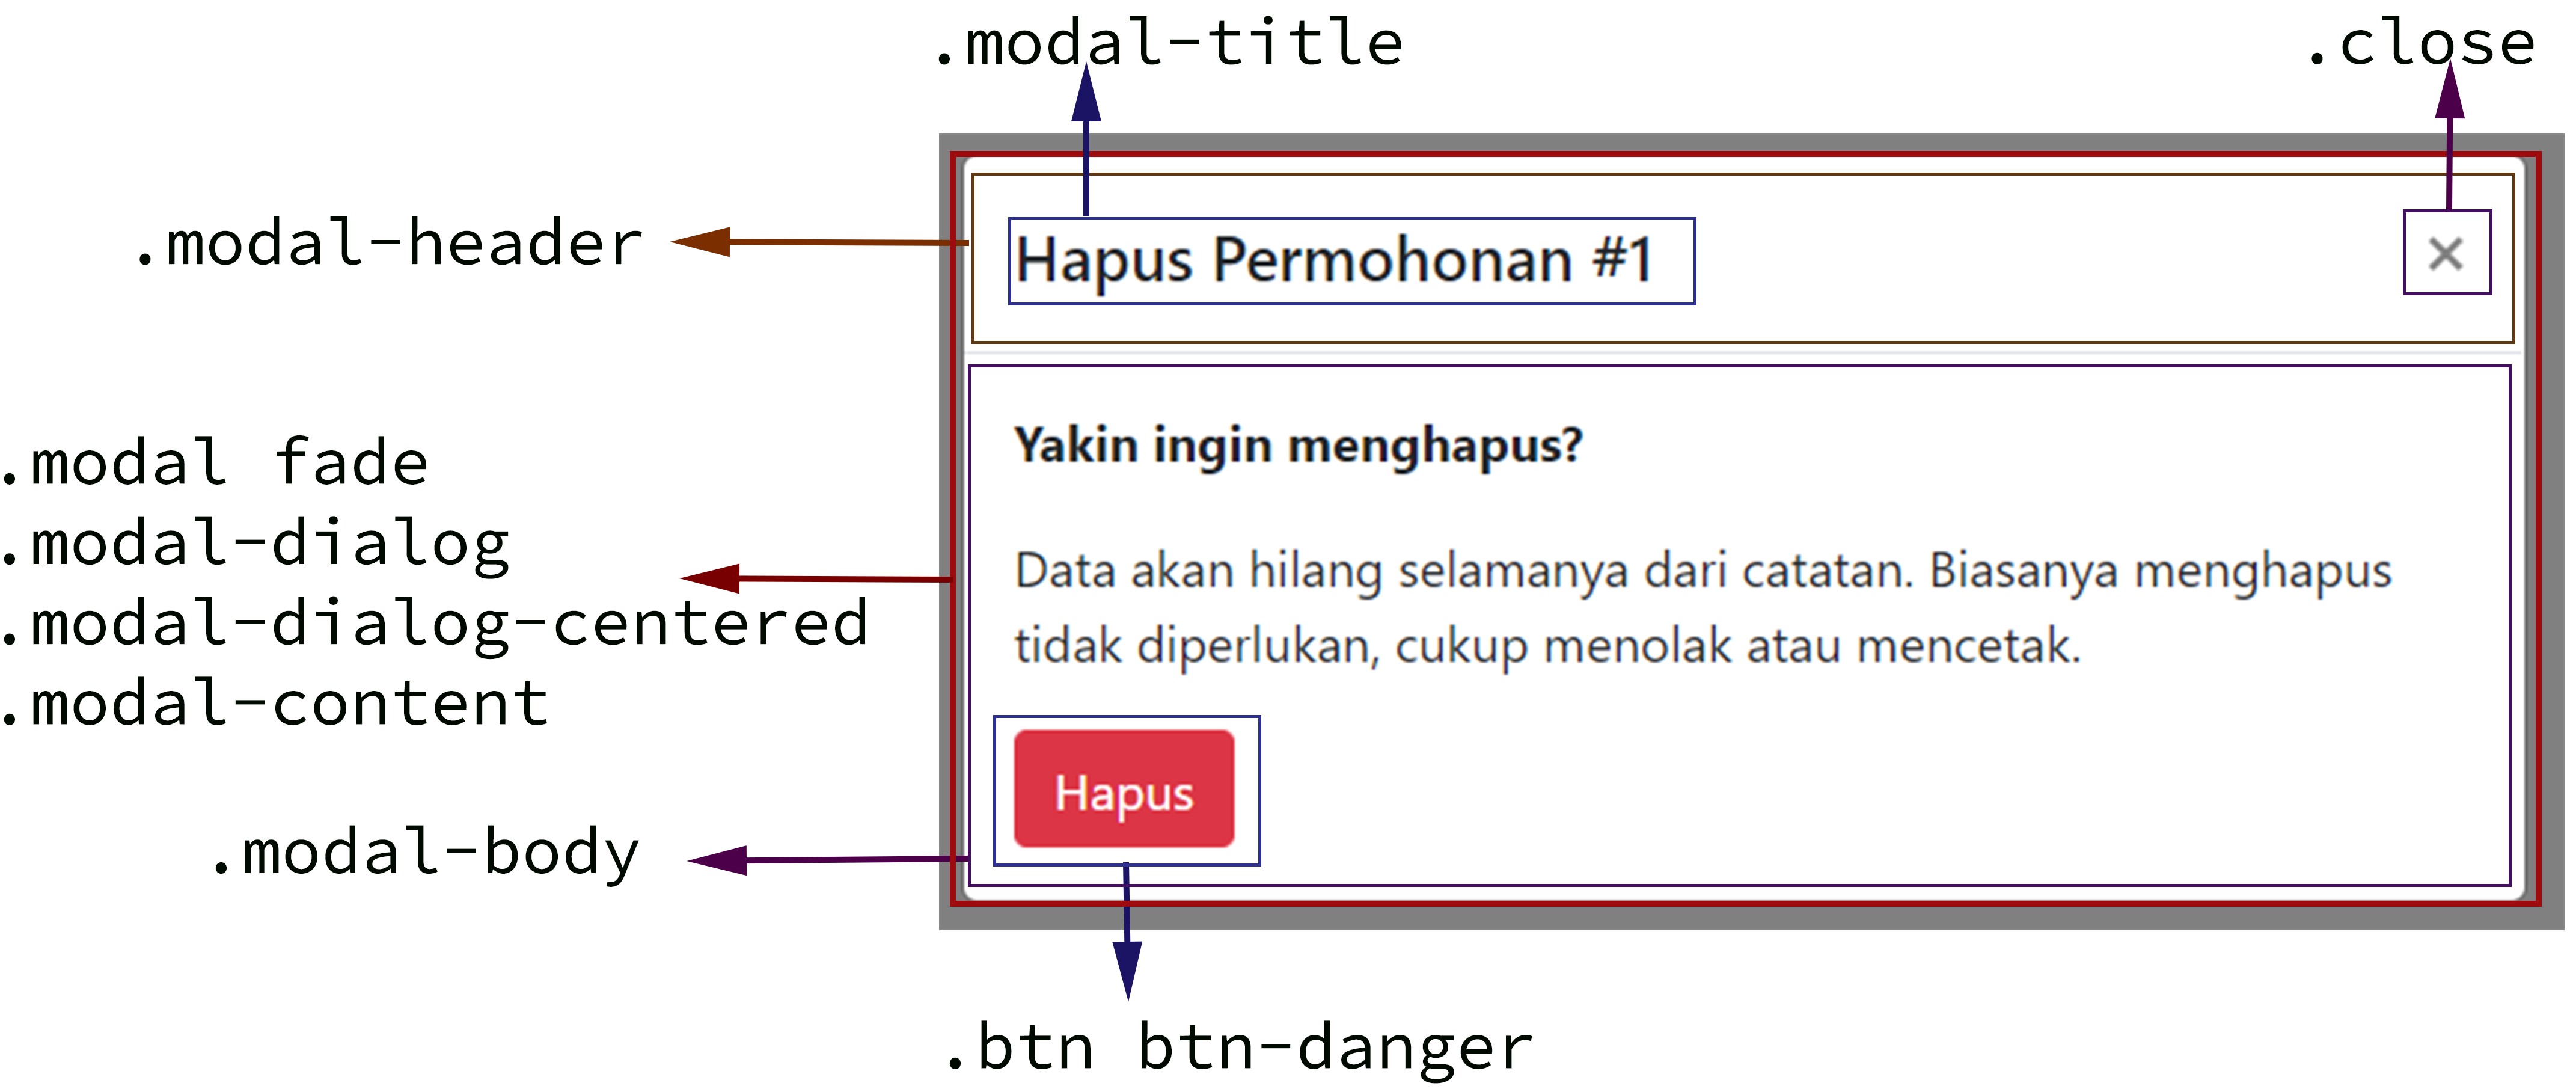
\includegraphics[width=\textwidth,height=\textheight,keepaspectratio]{bootstrap/konversi_modal_trash_manajemen_cetak_transkrip.png}
		\caption{Konversi Modal Hapus} 
	\end{subfigure}
\end{figure}
\begin{lstlisting}[language=diff, caption=Kode untuk Modal Cetak Transkrip Manage, label=Entri, basicstyle=\ttfamily, frame=single,
columns=fullflexible, keepspaces=true, breaklines=true]
@@ Implementasi Komponen Modal, Form dan Tabel @@ 
- <div class="reveal" id="detail<?= $request->id ?>" data-reveal>
-                <h5>Detail Permohonan #<?= $request->id ?></h5>
-                <table class="stack">
+ <div class="modal fade" id="detail<?= $request->id ?>" tabindex="-1" role="dialog" aria-hidden="true">
+    <div class="modal-dialog modal-dialog-centered" role="document">
+        <div class="modal-content">
+            <div class="modal-header">
+                <h5 class="modal-title" id="exampleModalLongTitle">Detail Permohonan #<?= $request->id ?></h5>
+                <button type="button" class="close" data-dismiss="modal" aria-label="Close">
+                    <span aria-hidden="true">&times;</span>
+                </button>
+            </div>
+            <div class="modal-body">
+                <table class="table table-striped">

+            </div>
+        </div>
+    </div>
+ </div>
+ <a data-toggle="modal" data-target="#detail<?= $request->id ?>" id="detailIkon<?= $request->id ?>">
+    <i class="fas fa-eye"></i>
+ </a>
-                <button class="close-button" data-close aria-label="Tutup" type="button">
+ <div class="modal fade" id="tolak<?= $request->id ?>" tabindex="-1" role="dialog" aria-hidden="true">
+    <div class="modal-dialog modal-dialog-centered" role="document">
+        <div class="modal-content">
+            <div class="modal-header">
+                <h5 class="modal-title" id="exampleModalLongTitle">Tolak Permohonan #<?= $request->id ?></h5>
+                <button type="button" class="close" data-dismiss="modal" aria-label="Close">

@@ Implementasi Komponen Form @@
-  <label>Email penjawab:
-        <input type="text" value="<?= $answeredByEmail ?>" readonly="true"/>
-  </label>
-  <label>Alasan penolakan:
-        <input name="answeredMessage" class="input-group-field" type="text" required/>
-  </label>

+ <div class="form-group">
+  <label>Email penjawab:</label>
+  <input class="form-control" type="text" value="<?= $answeredByEmail ?>" readonly="true"/>
+ </div>
+ <div class="form-group">
+  <label>Alasan penolakan:</label>
+  <input class="form-control" name="answeredMessage" type="text" required/>
+ </div>

-     <input type="submit" class="alert button" value="Tolak"/>
+  <div class="form-group">
+     <input type="submit" class="btn btn-danger" value="Tolak"/>
+  </div>

+            </div>
+        </div>
+    </div>
+ </div>
+ <a data-toggle="modal" data-target="#tolak<?= $request->id ?>" id="detailIkon<?= $request->id ?>">
+    <i class="fas fa-thumbs-down"></i>
+ </a>

-                <button class="close-button" data-close aria-label="Tutup" type="button">
+ <div class="modal fade" id="cetak<?= $request->id ?>" tabindex="-1" role="dialog" aria-hidden="true">
+    <div class="modal-dialog modal-dialog-centered" role="document">
+        <div class="modal-content">
+            <div class="modal-header">
+                <h5 class="modal-title" id="exampleModalLongTitle">Cetak Permohonan #<?= $request->id ?></h5>
+                <button type="button" class="close" data-dismiss="modal" aria-label="Close">

@@ Implementasi Komponen Form @@
- <label>Email penjawab:
-	 <input type="text" value="<?= $answeredByEmail ?>" readonly="true"/>
- </label>
- <label>Keterangan tambahan:
-   <input name="answeredMessage" class="input-group-field" type="text" required/>
- </label>
+ <div class="form-group">
+   <label class="col-form-label">Email penjawab:</label>
+   <input class="form-control" type="text" value="<?= $answeredByEmail ?>" readonly="true"/>
+ </div>
+ <div class="form-group">
+   <label class="col-form-label">Keterangan tambahan:</label>
+   <input class="form-control" name="answeredMessage" type="text" required/>
+ </div>


@@ Implementasi Modal @@                                            
-  <input type="submit" class="button" value="Sudah dicetak"/>
+ <div class="form-group">
+  <input class="btn btn-primary" type="submit" class="button" value="Sudah dicetak"/>
+ </div>

+            </div>
+        </div>
+    </div>
+ </div>
+ <a data-toggle="modal" data-target="#cetak<?= $request->id ?>" id="detailIkon<?= $request->id ?>">
+    <i class="fas fa-print"></i>
+ </a>

- 		<button class="close-button" data-close aria-label="Tutup" type="button">
+ <div class="modal fade" id="hapus<?= $request->id ?>" tabindex="-1" role="dialog" aria-hidden="true">
+    <div class="modal-dialog modal-dialog-centered" role="document">
+        <div class="modal-content">
+            <div class="modal-header">
+                <h5 class="modal-title" id="exampleModalLongTitle">Hapus Permohonan #<?= $request->id ?></h5>
+                <button type="button" class="close" data-dismiss="modal" aria-label="Close">

- <input type="submit" class="alert button" value="Hapus"/>
+ <input class="btn btn-danger" type="submit" value="Hapus"/>

- <a data-open="hapus<?= $request->id ?>"><i class="fi-trash"></i></a>
+ <a data-toggle="modal" data-target="#hapus<?= $request->id ?>" id="detailIkon<?= $request->id ?>">
+    <i class="fas fa-trash"></i>
+ </a>
\end{lstlisting}

\subsection{Halaman Perubahan Kuliah Request}
\subsubsection{Halaman Utama}
\begin{figure} [H]
	\centering  
	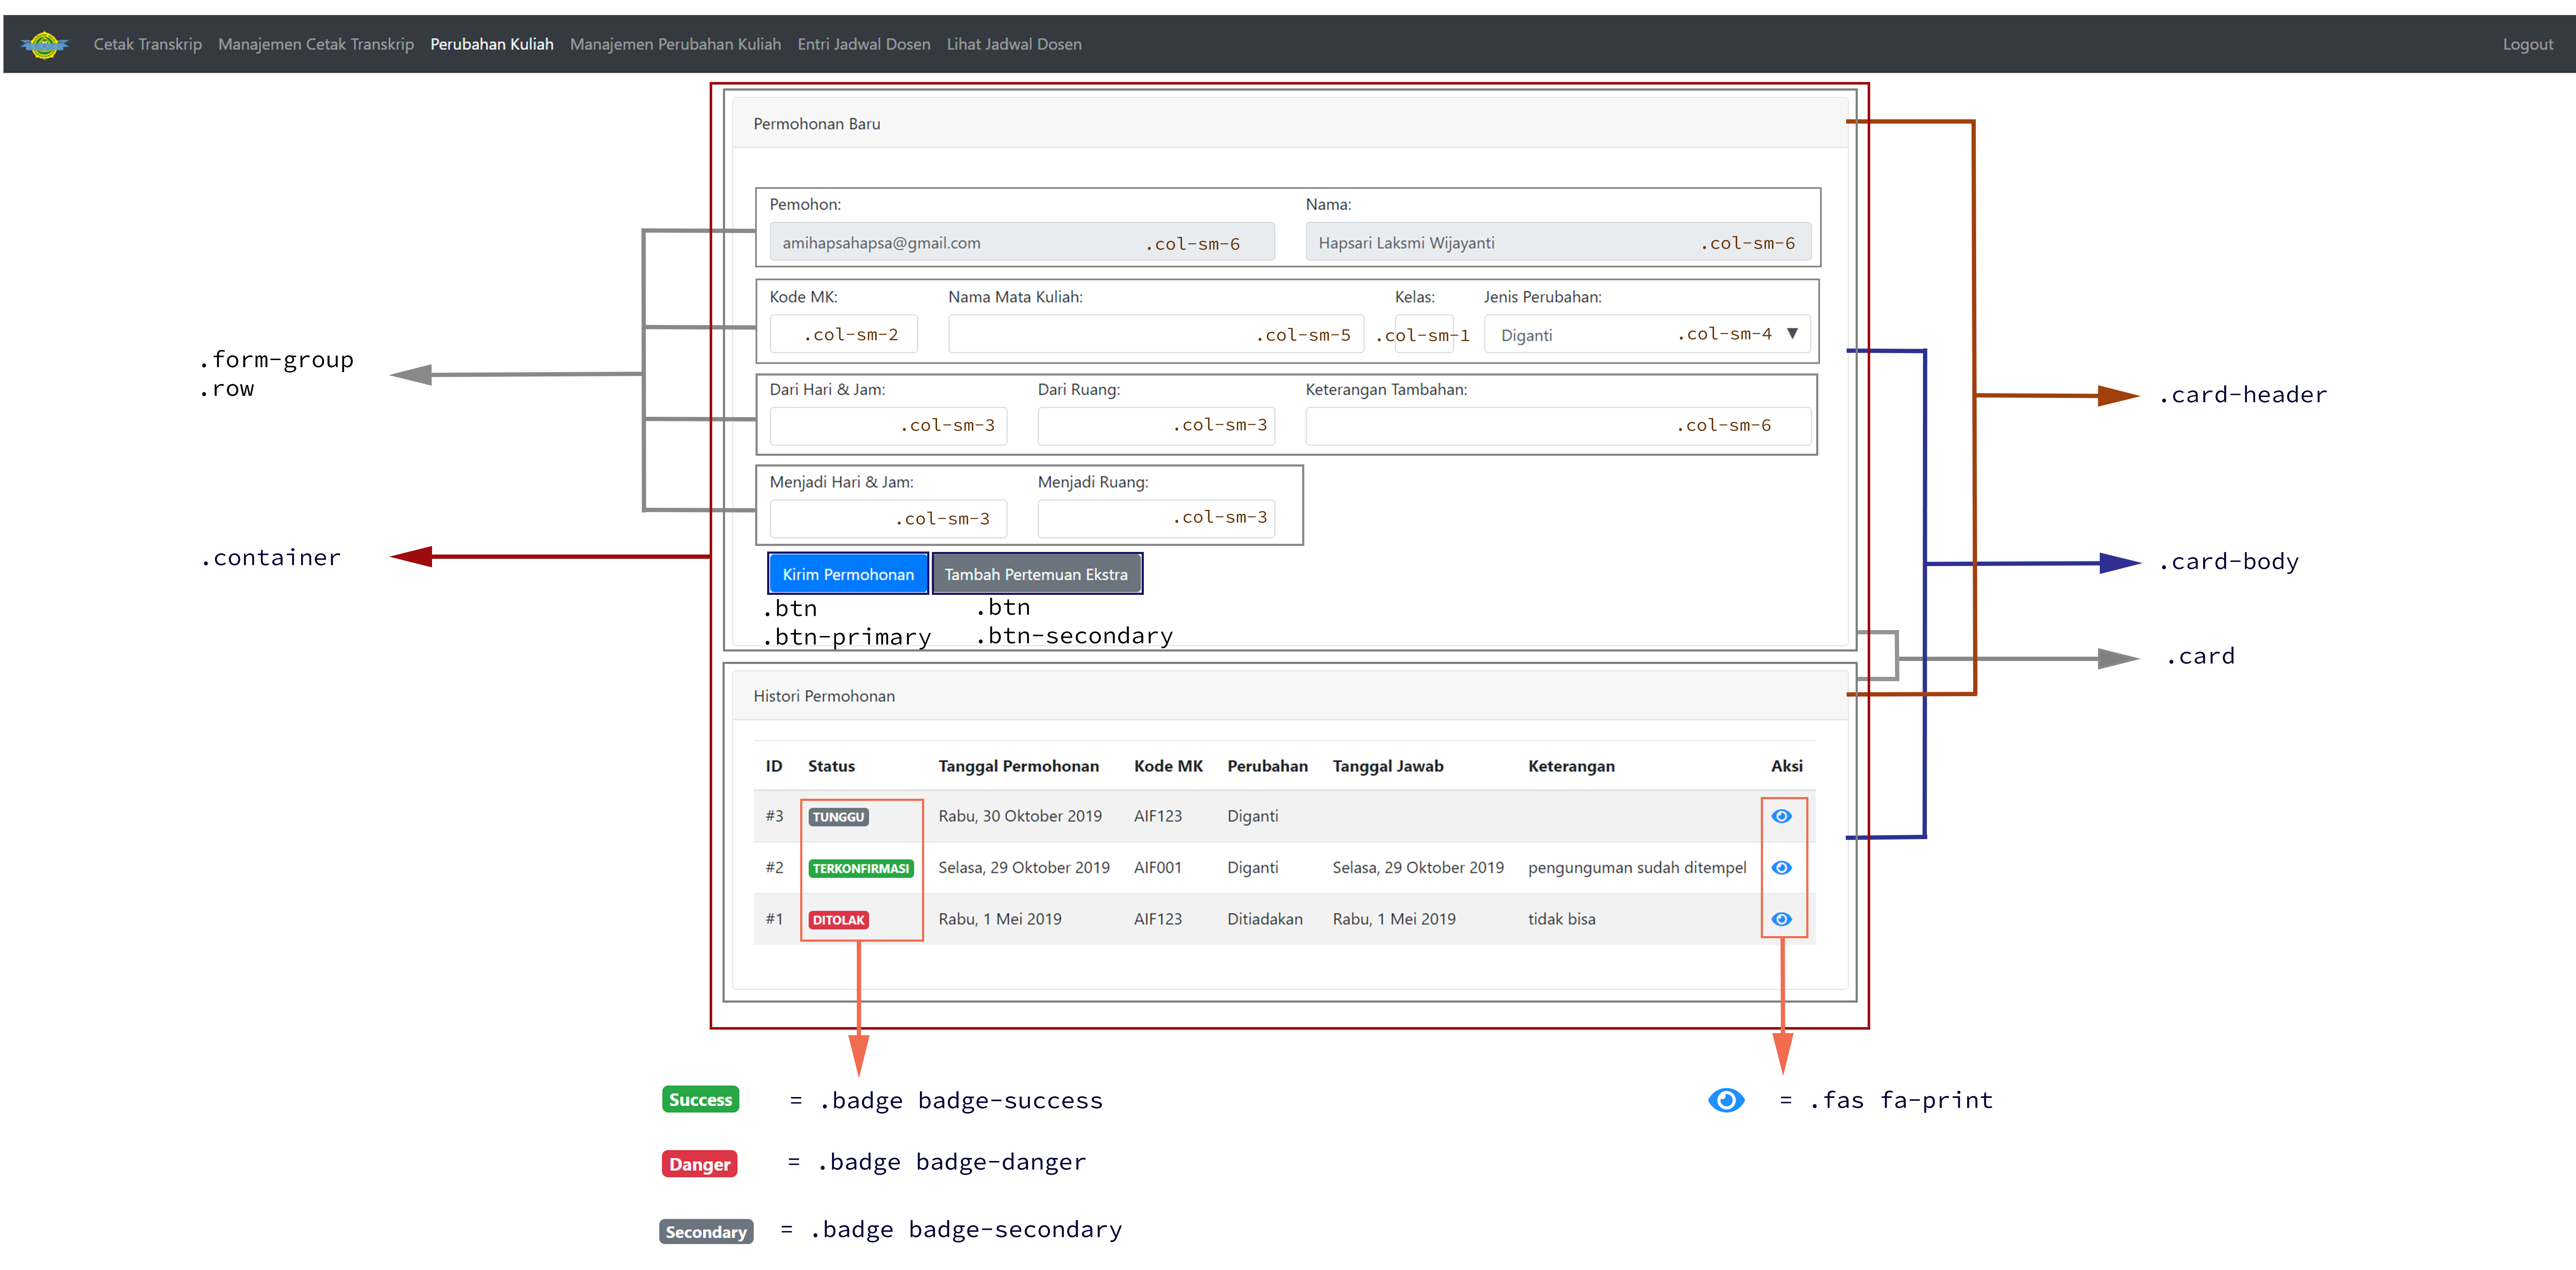
\includegraphics[width=\textwidth,height=\textheight,keepaspectratio]{bootstrap/konversi_tampilan_perubahan_kuliah.png}
	\caption{Konversi Halaman Perubahan Kuliah Request}
\end{figure}
\begin{lstlisting}[language=diff, caption=Kode untuk Halaman Perubahan Kuliah Request, label=Entri, basicstyle=\ttfamily, frame=single,
columns=fullflexible, keepspaces=true, breaklines=true]
--- C:\xampp\htdocs\BlueTape2\www\application\views\PerubahanKuliahRequest\main.php
+++ C:\xampp\htdocs\BlueTape\www\application\views\PerubahanKuliahRequest\main.php

@@ Implementasi Komponen Card @@
- <div class="row">
-    <div class="large-12 column">
-        <div class="callout">
-            <h5>Permohonan Baru</h5>
-            <form method="POST" action="/PerubahanKuliahRequest/add">
+        <div class="container">
+            <div class="card">
+                <div class="card-header">
+                    Permohonan Baru
+                </div>
+                <div class="card-body">
+                    <form class="p-3" method="POST" action="/PerubahanKuliahRequest/add">

@@ Implementasi Komponen Form @@
- <div class="row">
-    <div class="large-4 column">
-        <label>Pemohon:
-            <input type="email" name="requestByEmail" value="<?= $requestByEmail ?>" readonly="readonly"/>
-        </label>
+ <div class="form-group row">
+    <div class="col-sm-6">
+        <label class="col-form-label">Pemohon:</label>
+        <input class="form-control" type="email" name="requestByEmail" value="<?= $requestByEmail ?>" 

@@ Implementasi Komponen Form @@
- <div class="large-8 column">
- <label>Nama:
-    <input type="text" name="requestByName" value="<?= $requestByName ?>" readonly="readonly"/>
- </label>
+ <div class="col-sm-6">
+    <label class="col-form-label">Nama:</label>
+    <input class="form-control" type="text" name="requestByName" value="<?= $requestByName ?>" readonly="readonly"/>

@@ Implementasi Komponen Grid dan Form @@
- <div class="row">
-    <div class="large-2 column">
-        <label>Kode MK:
-            <input type="text" name="mataKuliahCode" required maxlength="9" pattern="[A-Z]{3}[0-9]{3}([0-9]{3})?" title="Kode MK dalam format XYZ123"/>
-        </label>
+  <div class="form-group row">
+     <div class="col-sm-2">
+        <label class="col-form-label">Kode MK:</label>
+        <input class="form-control" type="text" name="mataKuliahCode" required maxlength="9" pattern="[A-Z]{3}[0-9]{3}([0-9]{3})?" title="Kode MK dalam format XYZ123"/>

- <div class="large-5 column">
- <label>Nama Mata Kuliah:
-    <input type="text" name="mataKuliahName" required/>
- </label>
+ <div class="col-sm-5">
+    <label class="col-form-label">Nama Mata Kuliah:</label>
+    <input class="form-control" type="text" name="mataKuliahName" required/>

- <div class="large-1 column">
- <label>Kelas:
-    <input type="text" name="class" maxlength="1"/>
- </label>
+ <div class="col-sm-1">
+    <label class="col-form-label">Kelas:</label>
+    <input class="form-control" type="text" name="class" maxlength="1"/>

- <div class="large-4 column">
-   <label>Jenis Perubahan:
-    <select name="changeType">
+ <div class="col-sm-4">
+   <label class="col-form-label">Jenis Perubahan:</label>
+    <select name="changeType" class="form-control">

- <div class="row">
-    <div class="large-3 column">
-        <label>Dari Hari &amp; Jam:
-            <input class="disableable" type="text" name="fromDateTime" id="fromDateTime"/>
-        </label>
+ <div class="form-group row">
+    <div class="col-sm-3">
+        <label class="col-form-label">Dari Hari &amp; Jam:</label>
+        <input id="datetimepicker" class="form-control disableable" type="text" name="fromDateTime">

-    <div class="large-3 column">
-        <label>Dari Ruang:
-            <input class="disableable" type="text" name="fromRoom"/>
-        </label>
+   <div class="col-sm-3">
+        <label class="col-form-label">Dari Ruang:</label>
+        <input class="form-control disableable" type="text" name="fromRoom"/>

-    <div class="large-6 column">
-        <label>Keterangan Tambahan:
-            <input class="disableable" type="text" name="remarks"/>
-        </label>
+        <div class="col-sm-6">
+            <label class="col-form-label">Keterangan Tambahan:</label>
+            <input class="form-control disableable" type="text" name="remarks"/>

- <div class="row toFields">
-    <div class="large-3 column">
-        <label>Menjadi Hari &amp; Jam:
-            <input class="disableable toDateTime" type="text" name="toDateTime[]"/>
-        </label>
+    <div class="form-group row toFields">
+      <div class="col-sm-3">
+            <label class="col-form-label">Menjadi Hari &amp; Jam:</label>
+            <input id="datetimepicker" class="form-control disableable toDateTime" type="text" name="toDateTime[]"/>

-    <div class="large-3 column">
-        <label>Menjadi Ruang:
-            <input class="disableable toRoom" type="text" name="toRoom[]"/>
-        </label>
+    <div class="col-sm-3">
+        <label class="col-form-label">Menjadi Ruang:</label>
+        <input class="form-control disableable toRoom" type="text" name="toRoom[]"/>

-    <div class="large-6 column">
-        <br/>
-        <a href="#" class="eraseButton button secondary">Hapus</a>
+    <div class="col-sm-2">
+        <br/><br>
+        <a href="#" class="eraseButton btn btn-secondary">Hapus</a>

- <div class="row" id="sendDiv">
-    <div class="large-12 column">
-        <input type="submit" class="button" value="Kirim Permohonan">
-        <a href="#" id="addToButton" class="button secondary">Tambah Pertemuan Ekstra</a>
+    <div class="form-group row" id="sendDiv">
+      <div class="col-sm-12">
+        <input type="submit" class="btn btn-primary" value="Kirim Permohonan">
+        <a href="#" id="addToButton" class="btn btn-secondary">Tambah Pertemuan Ekstra</a>

@@ Implementasi Komponen Card dan Tabel @@
- <div class="callout">
- <h5>Histori Permohonan</h5>
- <table class="stack">
+ </div>
+  <br>
+ <div class="card">
+    <div class="card-header">
+      Histori Permohonan
+ </div>
+ <div class="card-body">
+    <table class="table table-striped table-responsive">

@@ Implementasi Kelas pada Elemen <th> @@
-        <th>ID</th>
-        <th>Status</th>
-        <th>Tanggal Permohonan</th>
-        <th>Kode MK</th>
-        <th>Perubahan</th>
-        <th>Tanggal Jawab</th>
-        <th>Keterangan</th>
-        <th>Aksi</th>
+        <th scope="col">ID</th>
+        <th scope="col">Status</th>
+        <th scope="col">Tanggal Permohonan</th>
+        <th scope="col">Kode MK</th>
+        <th scope="col">Perubahan</th>
+        <th scope="col">Tanggal Jawab</th>
+        <th scope="col">Keterangan</th>
+        <th scope="col">Aksi</th>

@@ Implementasi Badges @@
-  <td><span class="<?= $request->labelClass ?> label"><?= $request->status ?></span></td>
+  <td><span class=" badge badge-<?= $request->labelClass ?>"><?= $request->status ?></span></td>
\end{lstlisting}

\subsubsection{Modal}
%Lihat
\begin{figure} [H]
	\centering  
	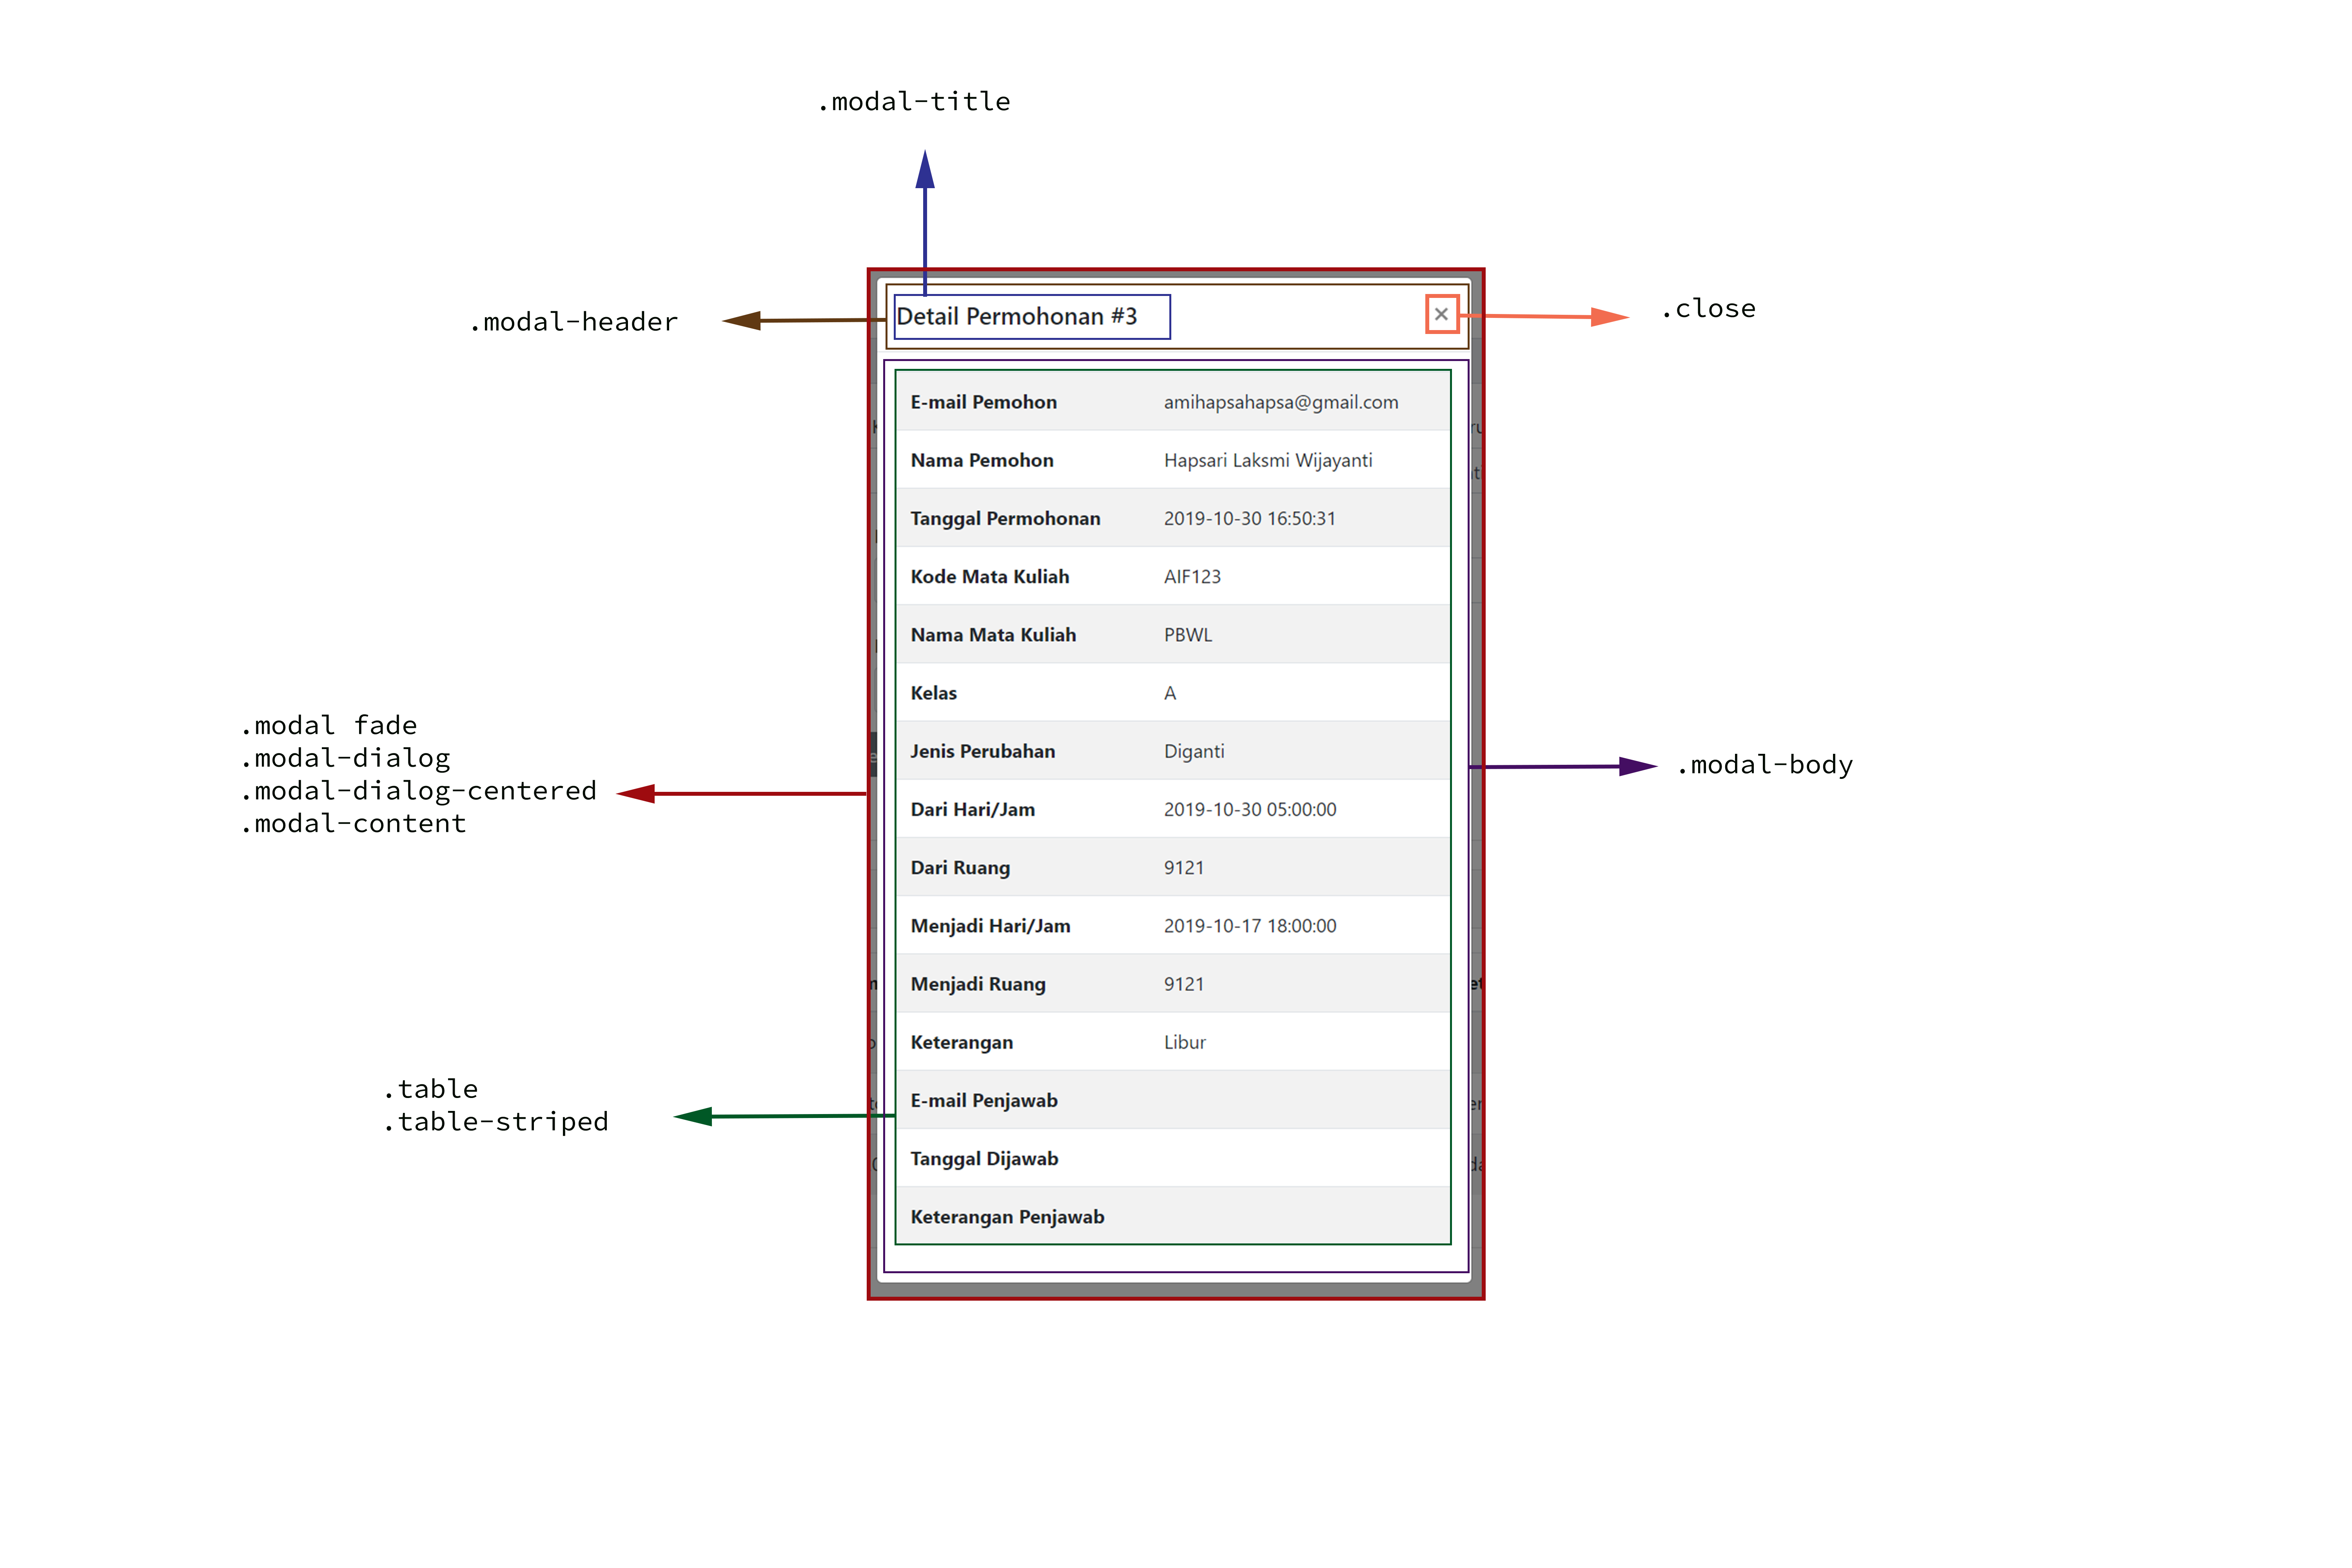
\includegraphics[width=\textwidth,height=\textheight,keepaspectratio]{bootstrap/konversi_modal_lihat_perubahan_kuliah.png}
	\caption{Konversi Modal Lihat Perubahan Kuliah Request}
\end{figure}
\begin{lstlisting}[language=diff, label=Entri, basicstyle=\ttfamily, frame=single,
columns=fullflexible, keepspaces=true, breaklines=true]

@@ Implementasi Ikon Font Awesome @@
-  <a data-open="detail<?= $request->id ?>"><i class="fi-eye"></i></a>
+  <a data-toggle="modal" data-target="#detail<?= $request->id ?>" id="detailIkon<?= $request->id ?>">
+     <span style="font-size: 18px; color: Dodgerblue;">
+        <i class="fas fa-eye"></i>
+     </span>
+     </a>

@@ Implementasi Komponen Modal @@
-    <div class="reveal" id="detail<?= $request->id ?>" data-reveal>
-        <h5>Detail Permohonan #<?= $request->id ?></h5>
-        <table class="stack">
+    <div class="modal fade" id="detail<?= $request->id ?>" tabindex="-1" role="dialog" aria-hidden="true">
+     <div class="modal-dialog modal-dialog-centered" role="document">
+        <div class="modal-content">
+           <div class="modal-header">
+              <h5 class="modal-title" id="exampleModalLongTitle">Detail Permohonan #<?= $request->id ?></h5>
+              <button type="button" class="close" data-dismiss="modal" aria-label="Close">
+                 <span aria-hidden="true">&times;</span>
+              </button>
+           </div>
+           <div class="modal-body">
+             <table class="table table-striped">
\end{lstlisting}

\subsection{Halaman Manajemen Perubahan Kuliah}
\subsubsection{Halaman Utama}
\begin{figure} [H]
	\centering  
	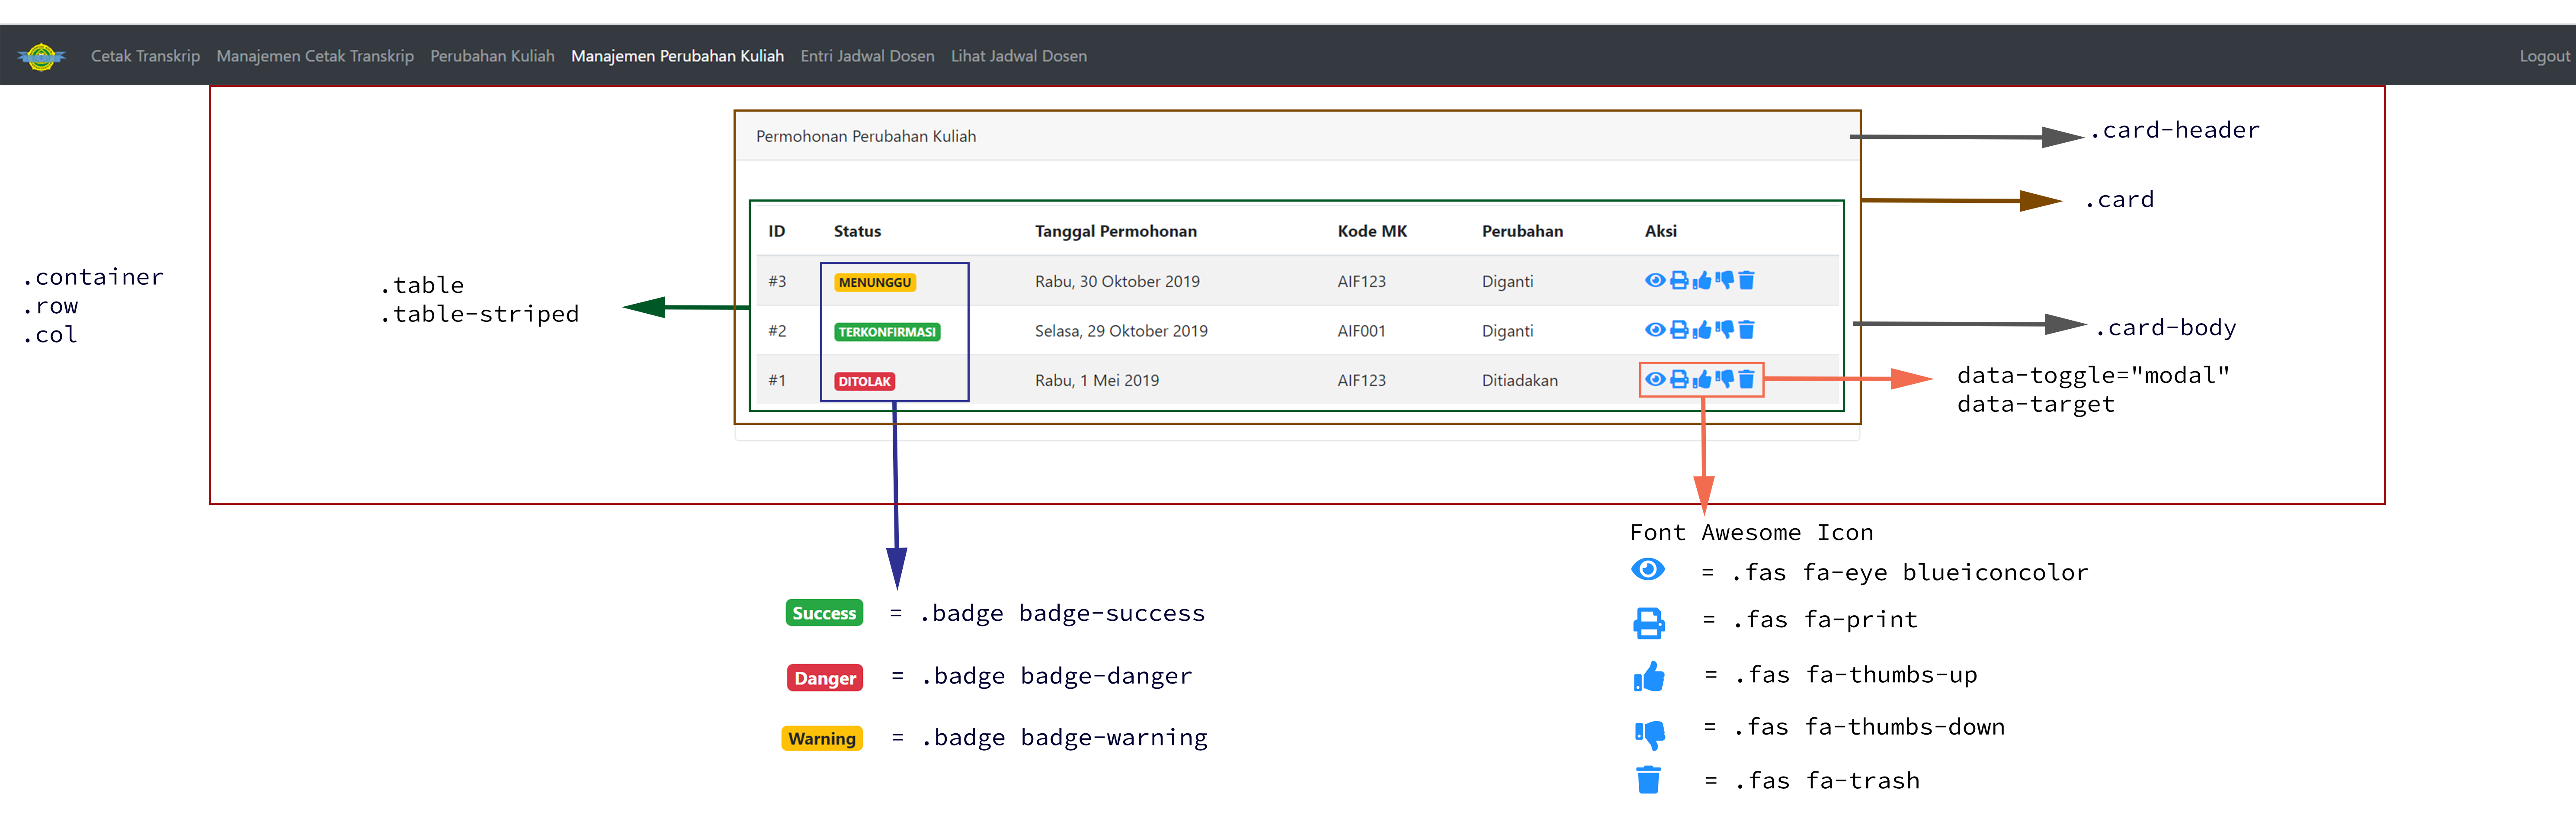
\includegraphics[width=\textwidth,height=\textheight,keepaspectratio]{bootstrap/konversi_tampilan_manajemen_perubahan_kuliah.png}
	\caption{Konversi Halaman Manajemen Perubahan Kuliah}
\end{figure}
\begin{lstlisting}[language=diff, caption=Kode untuk Halaman Manajemen Perubahan Kuliah, label=Entri, basicstyle=\ttfamily, frame=single,
columns=fullflexible, keepspaces=true, breaklines=true]
--- C:\xampp\htdocs\BlueTape2\www\application\views\PerubahanKuliahManage\main.php
+++ C:\xampp\htdocs\BlueTape\www\application\views\PerubahanKuliahManage\main.php00

@@ Implementasi Komponen Card @@
- <div class="row">
-    <div class="callout">
-        <h5>Permohonan Perubahan Kuliah</h5>
-        <table class="stack">
+        <div class="container">
+            <div class="card">
+                <div class="card-header">
+                    Permohonan Perubahan Kuliah
+                </div>
+                <br>
+                <div class="card-body">
+                    <table class="table table-striped">

@@ Implementasi Kelas Column pada elemen <th> @@
- <th>ID</th>
- <th>Status</th>
- <th>Tanggal Permohonan</th>
- <th>Kode MK</th>
- <th>Perubahan</th>
- <th>Aksi</th>
+ <th scope="col">ID</th>
+ <th scope="col">Status</th>
+ <th scope="col">Tanggal Permohonan</th>
+ <th scope="col">Kode MK</th>
+ <th scope="col">Perubahan</th>
+ <th scope="col">Aksi</th>

@@ Implementasi Komponen Badge @@
- <td><span class="<?= $request->labelClass ?> label"><?= $request->status ?></span></td>
+ <td><span class="badge badge-<?= $request->labelClass ?>"><?= 

@@ Implementasi Komponen Form @@
-   <label>Email penjawab:
-    <input type="text" value="<?= $answeredByEmail ?>" readonly="true"/>
-   </label>
-   <label>Keterangan:
-    <input name="answeredMessage" class="input-group-field" type="text"/>
-   </label>
+ <div class="form-group">
+   <label>Email penjawab:</label>
+   <input class="form-control" type="text" value="<?= $answeredByEmail ?>" readonly="true"/>
+ </div>
+ <div class="form-group">
+   <label>Keterangan:</label>
+   <input class="form-control" name="answeredMessage" class="input-group-field" type="text"/>
+ </div>

@@ Implementasi Komponen Button @@                                            
-    	<input type="submit" class="success button" value="Konfirmasi"/>
+    <div class="form-group">
+       <input type="submit" class="btn btn-success" value="Konfirmasi"/>
+    </div>
</form>
\end{lstlisting}
\subsubsection{Modal}
%Lihat Terima Tolak Print Hapus
\begin{figure}	
	\centering
	\begin{subfigure}[t]{3in}
		\centering  
		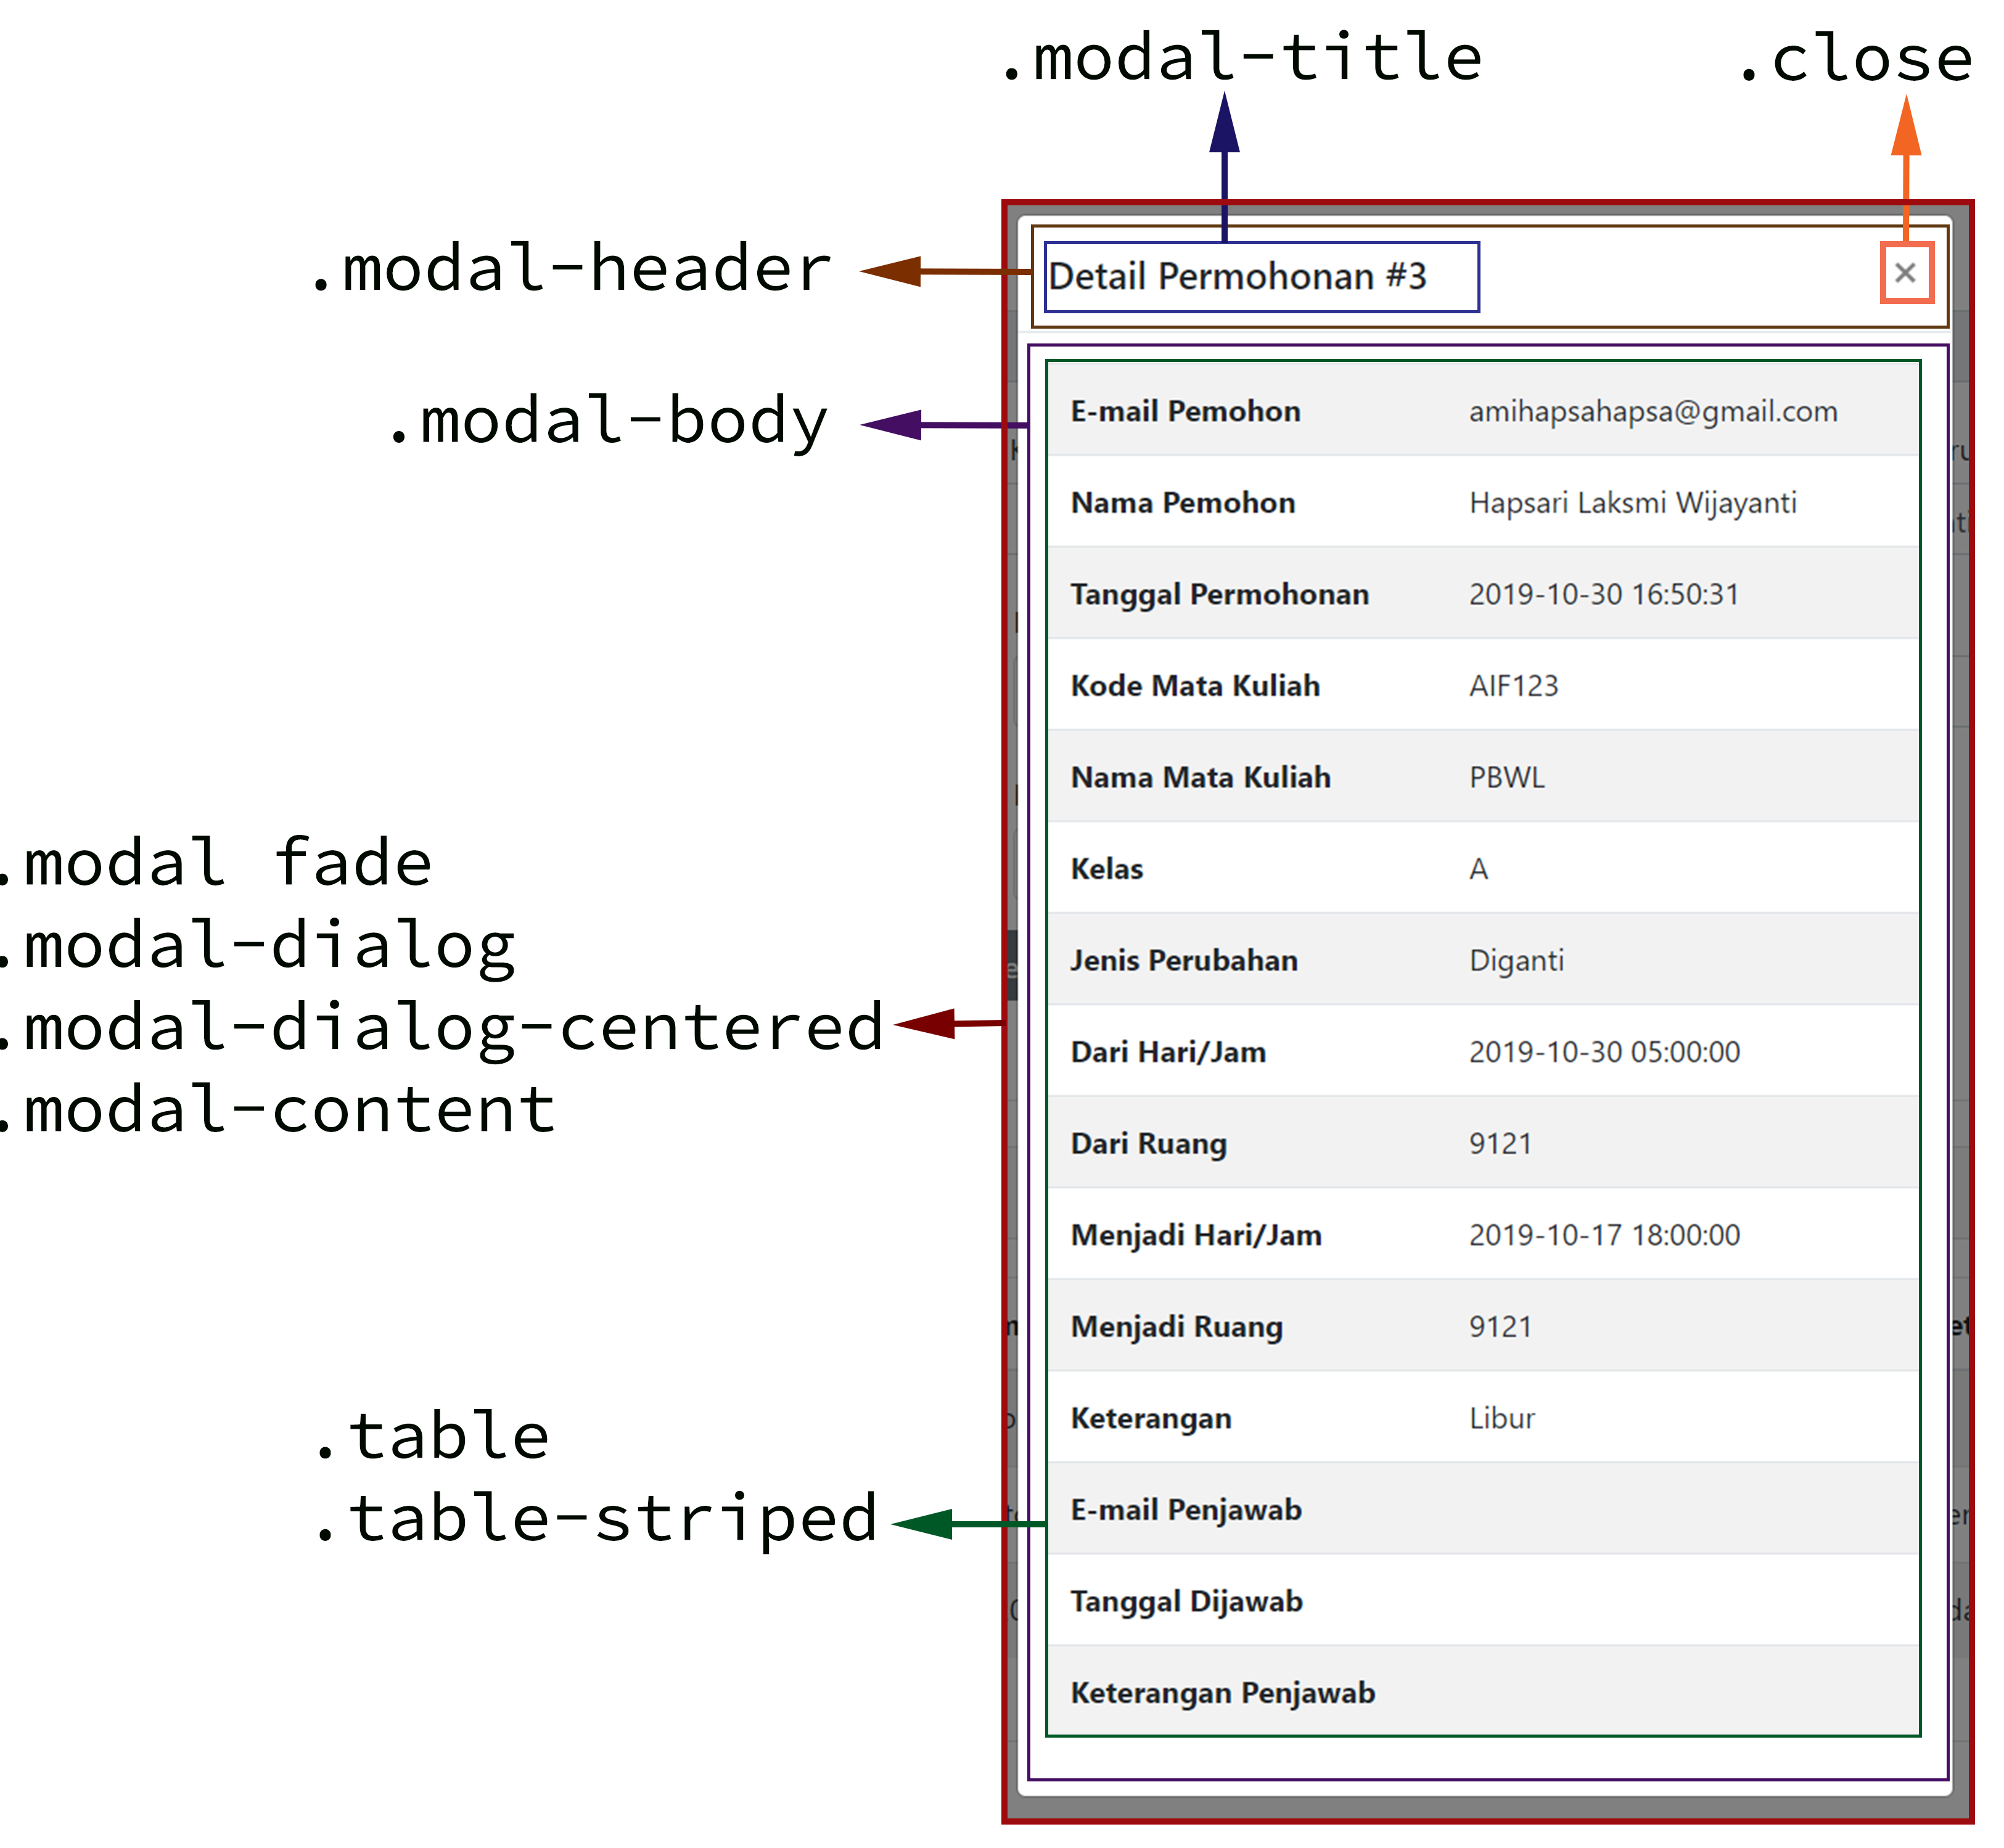
\includegraphics[width=\textwidth,height=\textheight,keepaspectratio]{bootstrap/konversi_modal_lihat_manajemen_perubahan_kuliah.png}
		\caption{Konversi Modal Lihat} 
	\end{subfigure}
	\quad
	\begin{subfigure}[t]{3in}
		\centering  
		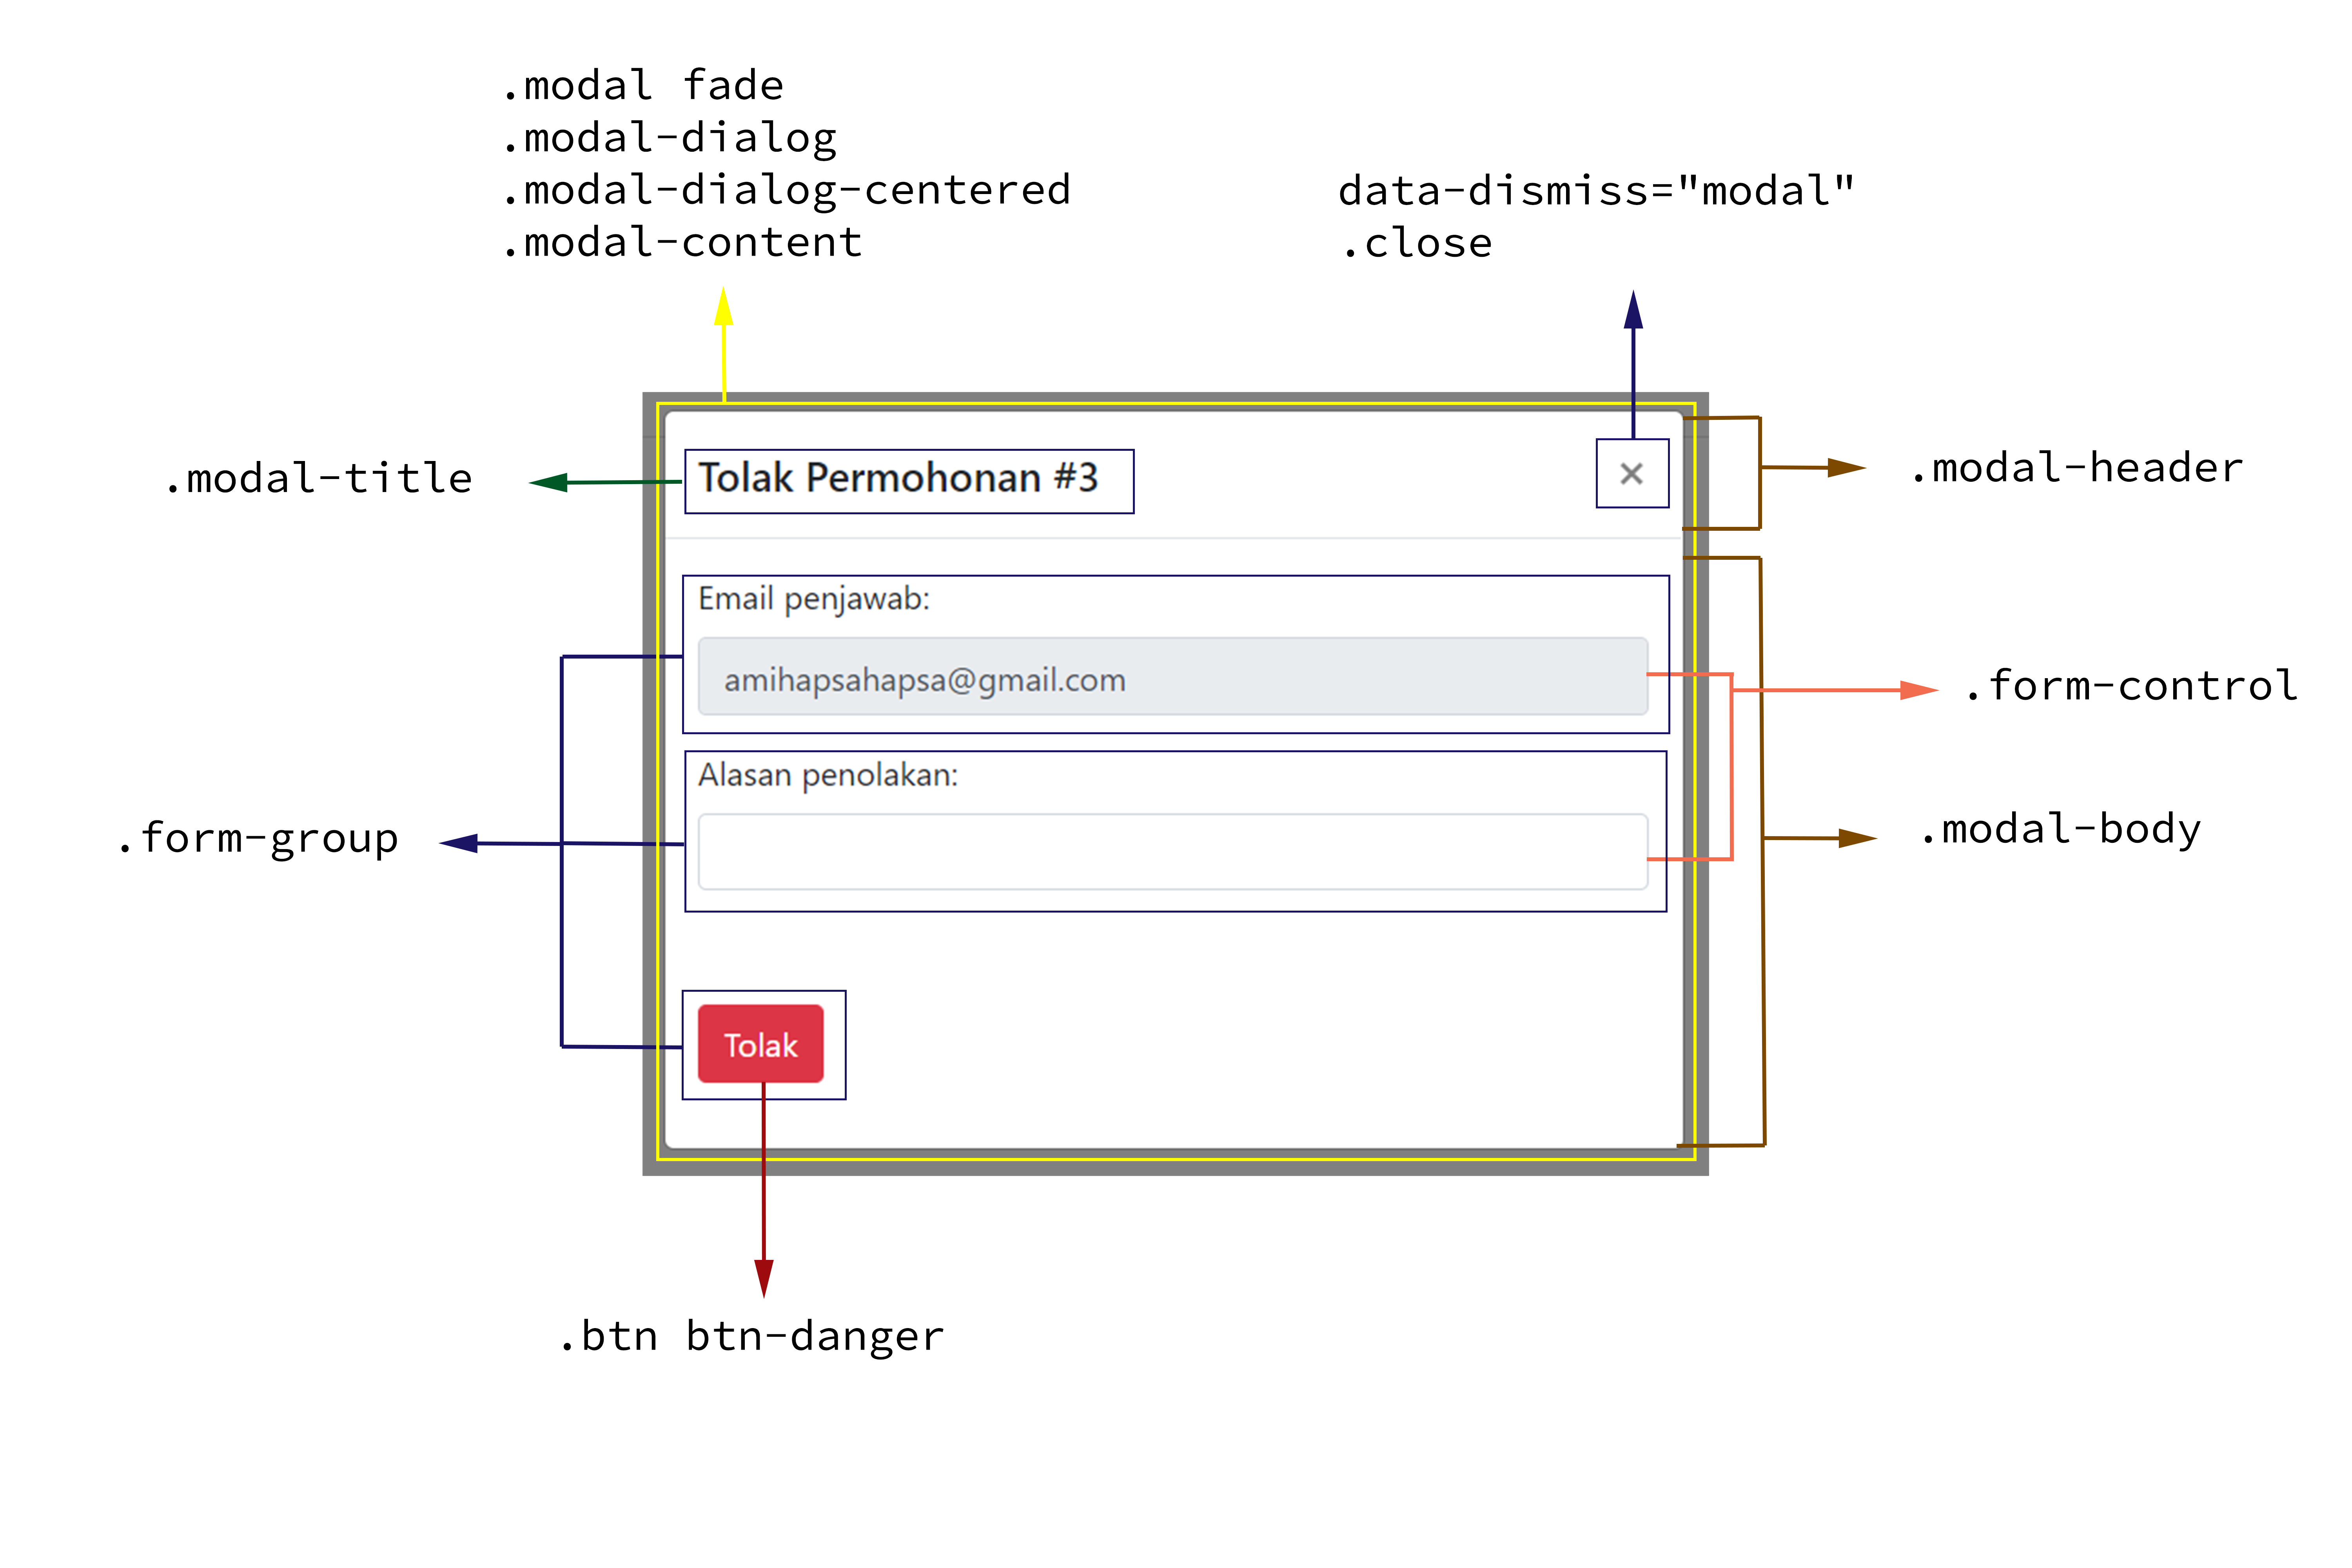
\includegraphics[width=\textwidth,height=\textheight,keepaspectratio]{bootstrap/konversi_modal_dislike_manajemen_perubahan_kuliah.png}
		\caption{Konversi Modal Tolak} 
	\end{subfigure}
\end{figure}
\begin{figure}	
	\centering
	\begin{subfigure}[t]{3in}
		\centering  
		\includegraphics[width=\textwidth,height=\textheight,keepaspectratio]{bootstrap/konversi_modal_print_manajemen_perubahan_kuliah.png}
		\caption{Konversi Modal Print} 
	\end{subfigure}
	\quad
	\begin{subfigure}[t]{3in}
		\centering  
		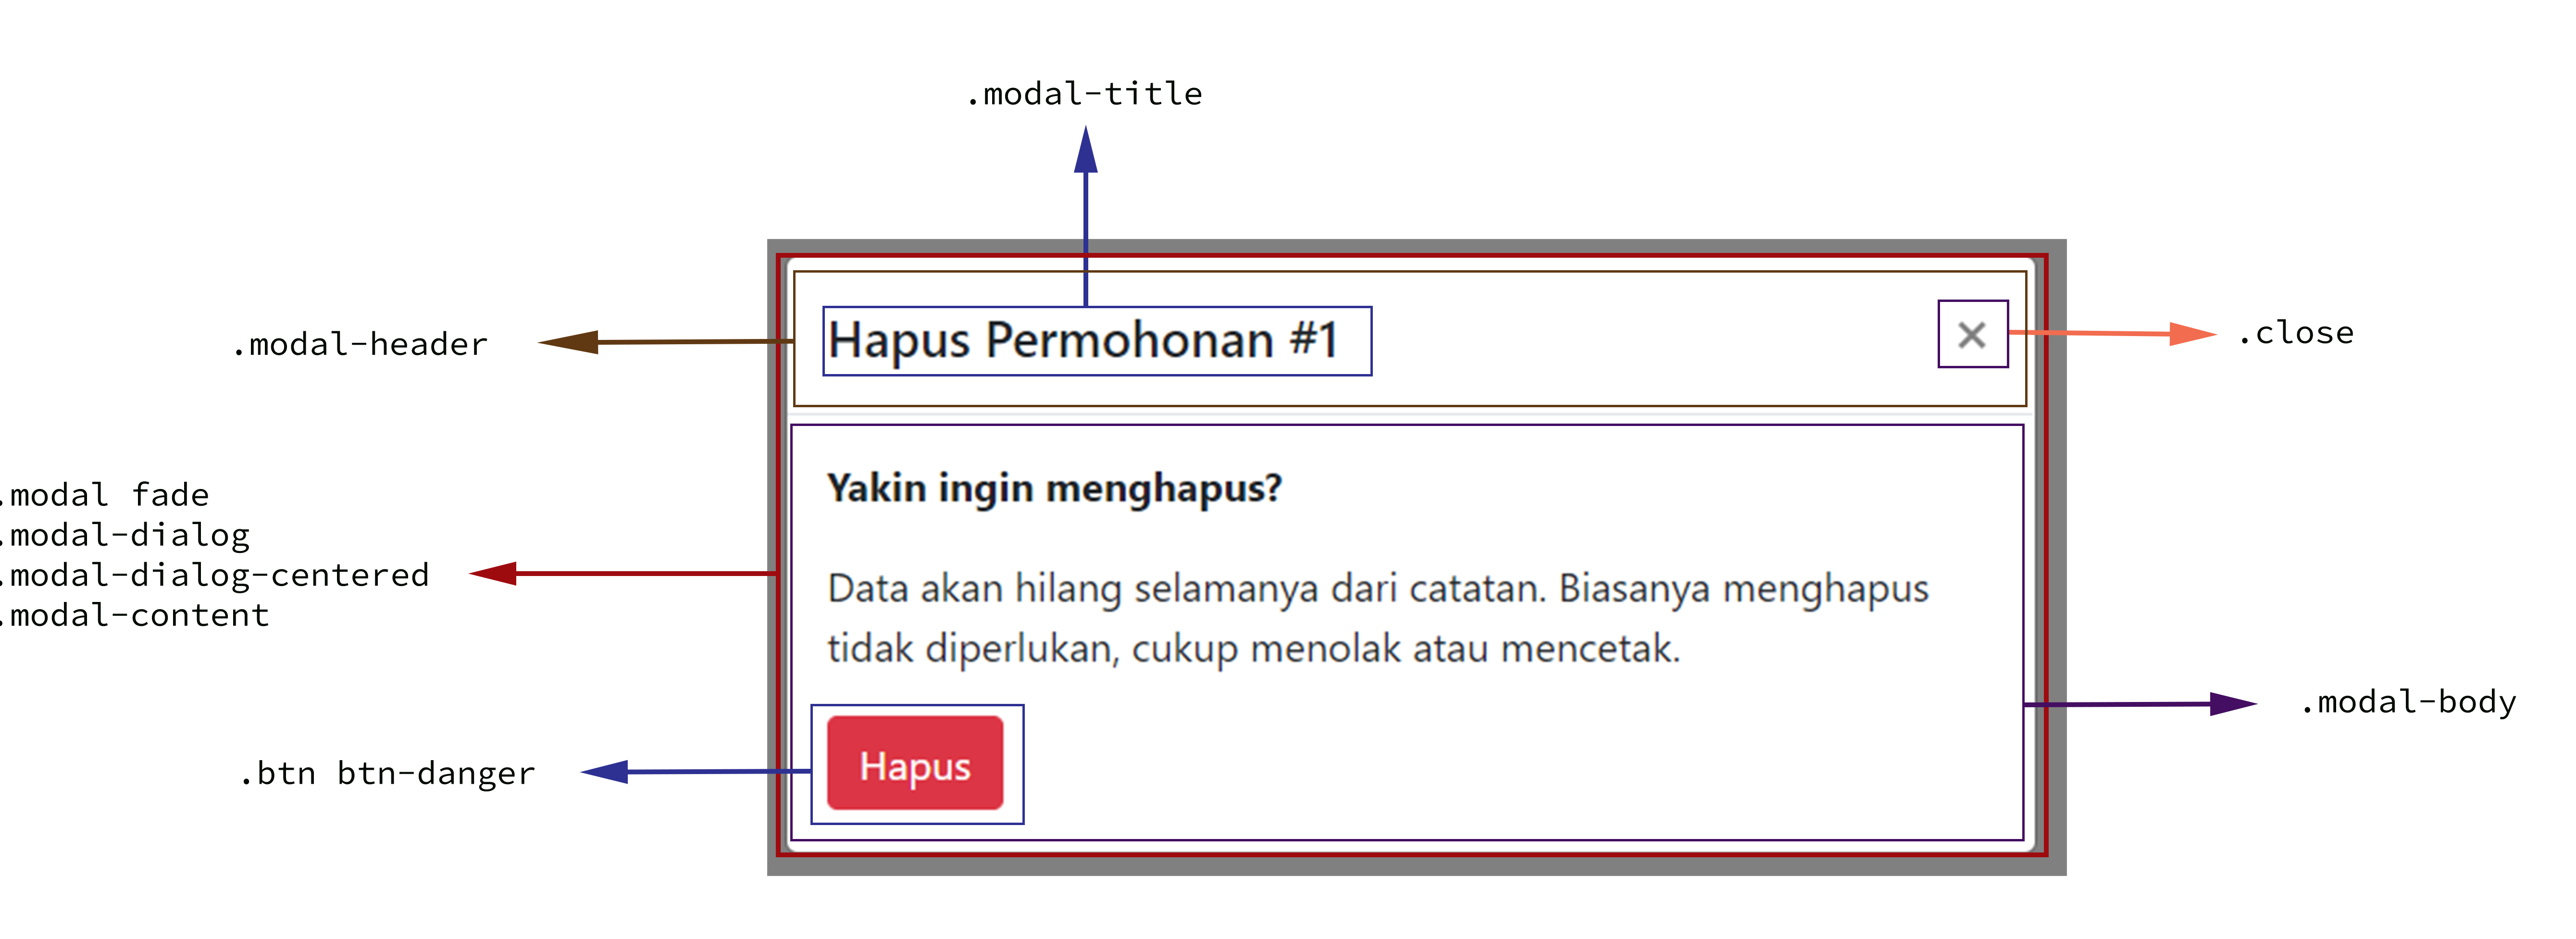
\includegraphics[width=\textwidth,height=\textheight,keepaspectratio]{bootstrap/konversi_modal_trash_manajemen_perubahan_kuliah.png}
		\caption{Konversi Modal Hapus} 
	\end{subfigure}
\end{figure}
\begin{figure}	
	\centering
	\begin{subfigure}[t]{3in}
		\centering  
		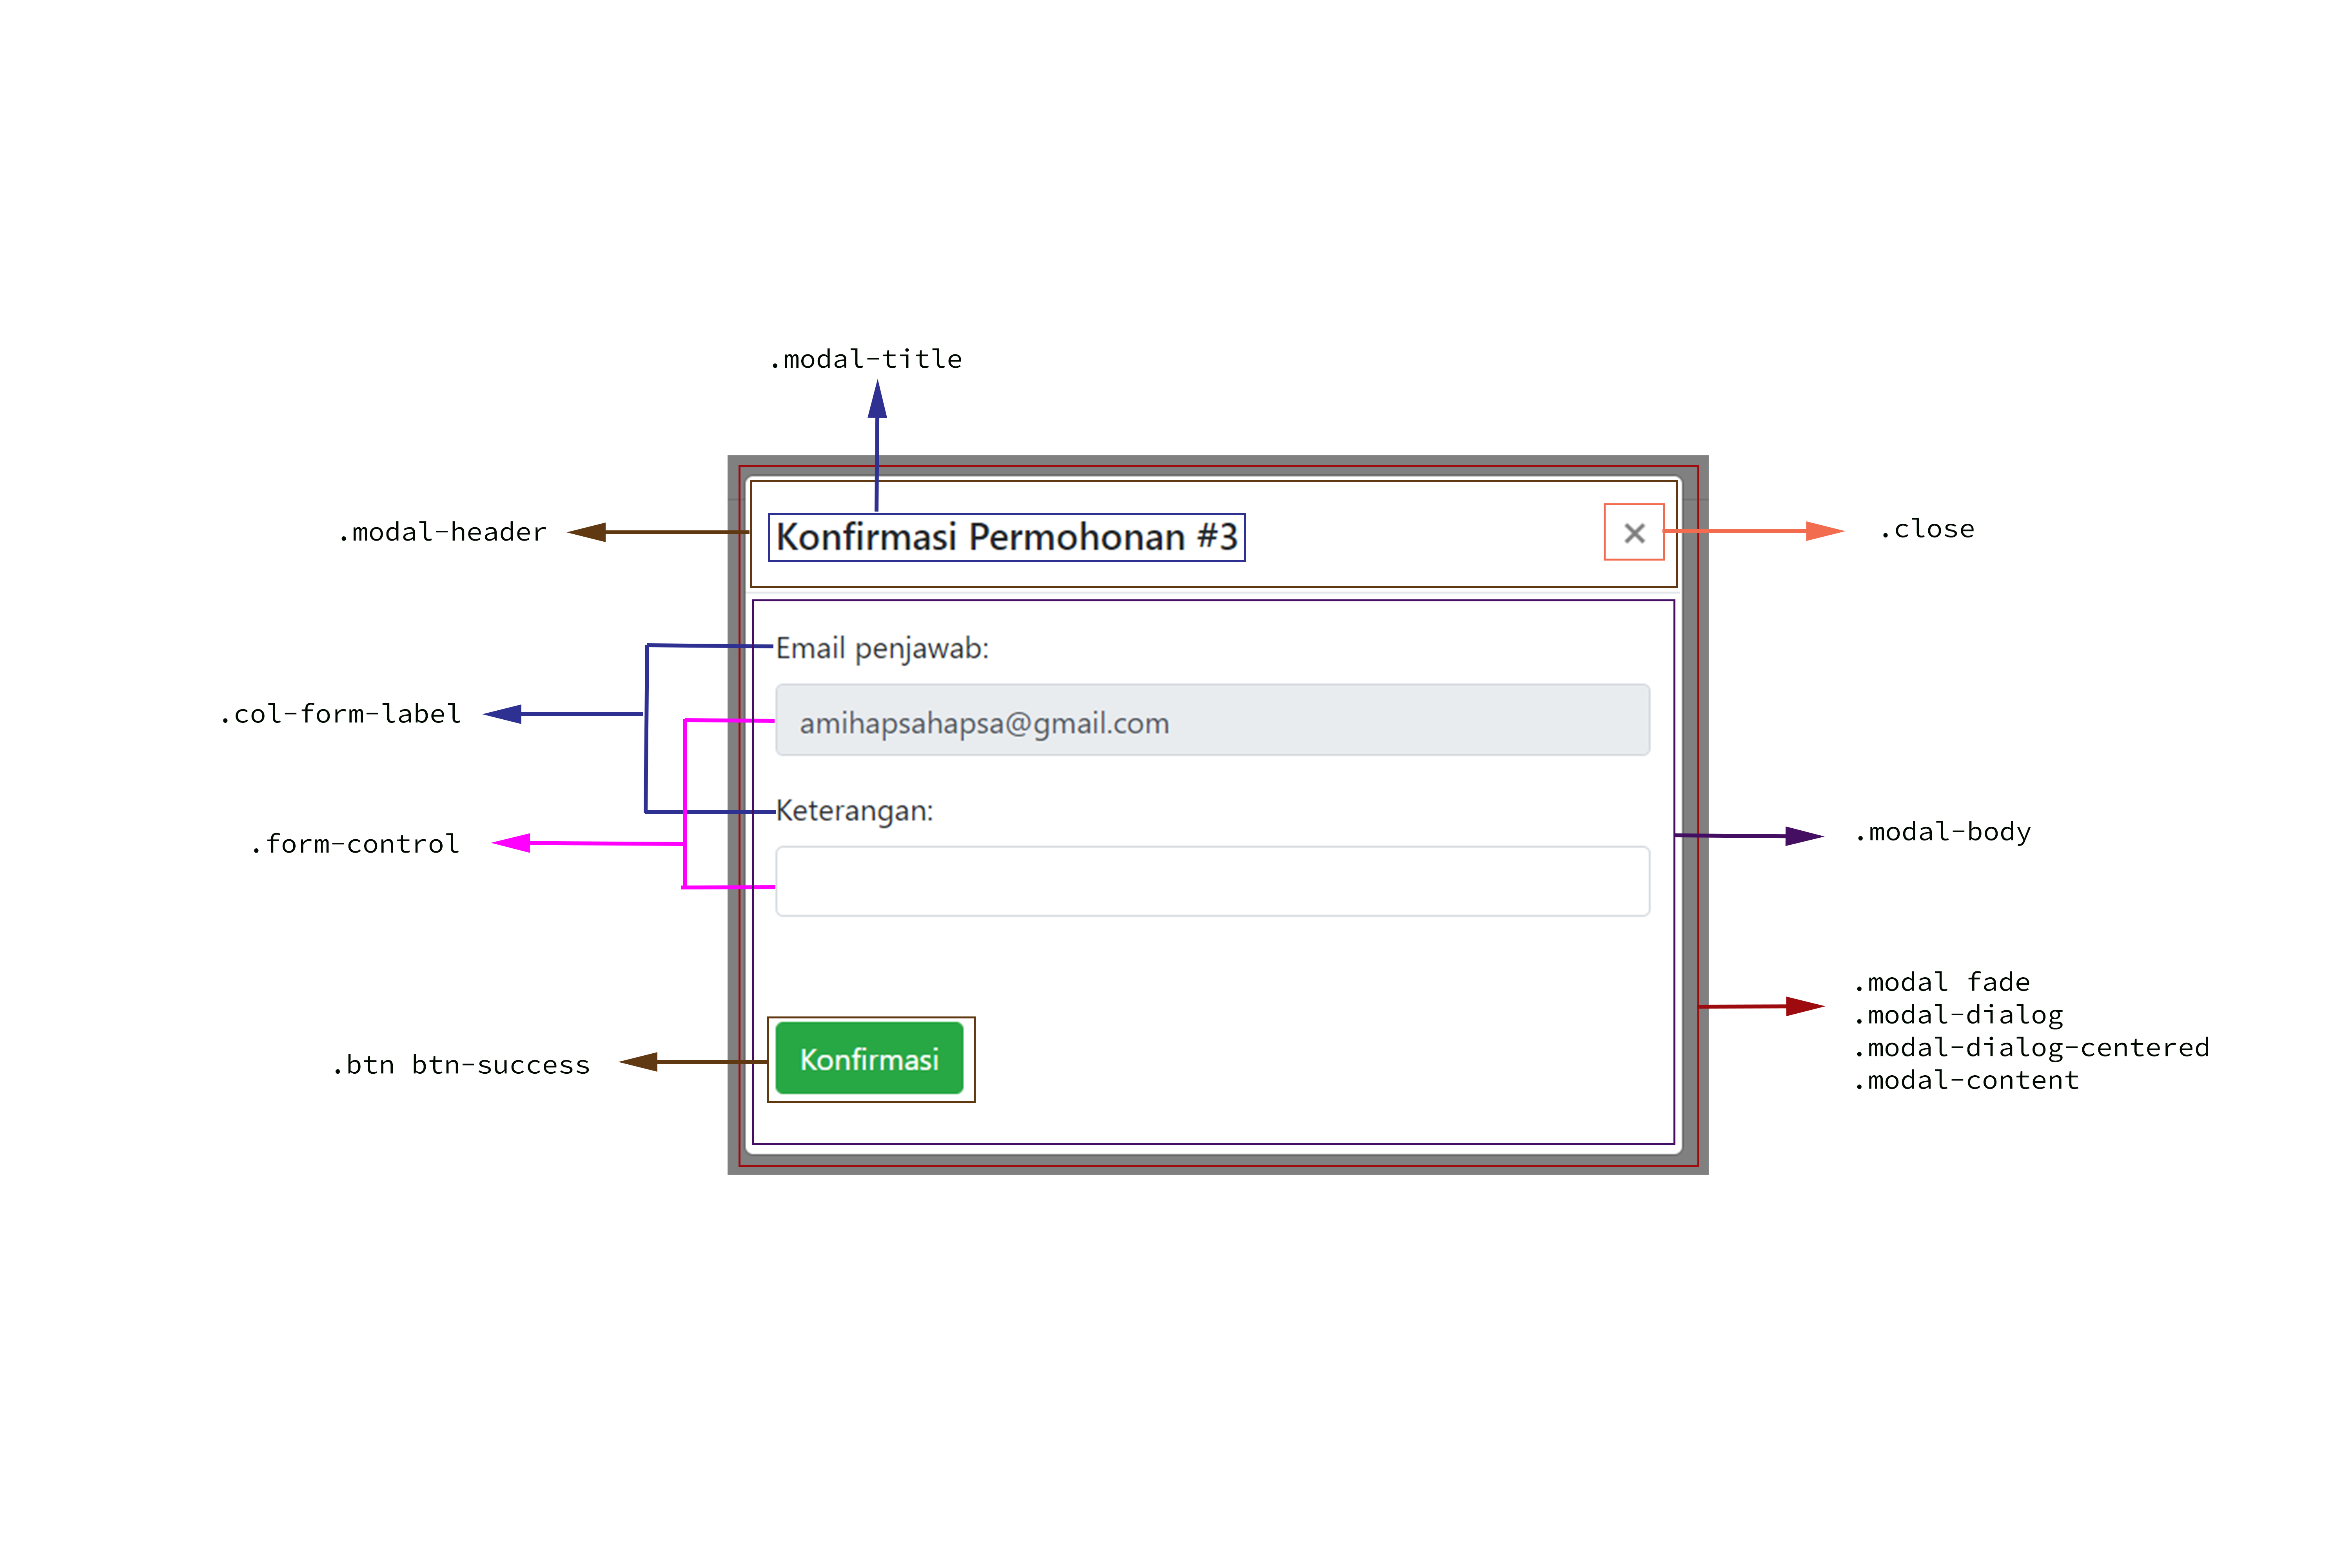
\includegraphics[width=\textwidth,height=\textheight,keepaspectratio]{bootstrap/konversi_modal_like_manajemen_perubahan_kuliah.png}
		\caption{Konversi Modal Like} 
	\end{subfigure}
\end{figure}
\begin{lstlisting}[language=diff, label=Entri, basicstyle=\ttfamily, frame=single,
columns=fullflexible, keepspaces=true, breaklines=true]
@@ Implementasi Komponen Modal dan Library Ikon Awesome @@
- <a data-open="detail<?= $request->id ?>"><i class="fi-eye"></i></a>
- <a target="_blank" href="/PerubahanKuliahManage/printview/<?= $request->id ?>"><i class="fi-print"></i></a>
- <a data-open="konfirmasi<?= $request->id ?>"><i class="fi-like"></i></a>                                    
- <a data-open="tolak<?= $request->id ?>"><i class="fi-dislike"></i></a>
- <a data-open="hapus<?= $request->id ?>"><i class="fi-trash"></i></a>
+ <a data-toggle="modal" data-target="#detail<?= $request->id ?>" id="detailIkon<?= $request->id ?>"><i class="fas fa-eye blueiconcolor"></i></a>
+ <a target="_blank" href="/PerubahanKuliahManage/printview/<?= $request->id ?>"><i class="fas fa-print"></i></a>
+ <a data-toggle="modal" data-target="#konfirmasi<?= $request->id ?>"><i class="fas fa-thumbs-up"></i></a>
+ <a data-toggle="modal" data-target="#tolak<?= $request->id ?>"><i class="fas fa-thumbs-down"></i></a>
+ <a data-toggle="modal" data-target="#hapus<?= $request->id ?>"><i 

@@ Implementasi Komponen  Modal @@
- <div class="reveal" id="detail<?= $request->id ?>" data-reveal>
- <h5>Detail Permohonan #<?= $request->id ?></h5>
- <table class="stack">
+ <div class="modal fade" id="detail<?= $request->id ?>" tabindex="-1" role="dialog" aria-hidden="true">
+    <div class="modal-dialog modal-dialog-centered" role="document">
+       <div class="modal-content">
+          <div class="modal-header">
+             <h5 class="modal-title" id="exampleModalLongTitle">Detail Permohonan #<?= $request->id ?></h5>
+             <button type="button" class="close" data-dismiss="modal" aria-label="Close">
+               <span aria-hidden="true">&times;</span>
+             </button>
+           </div>
+           <div class="modal-body">
+               <table class="table table-striped">

@@ Implementasi Komponen Modal @@
-               <button class="close-button" data-close aria-label="Tutup" type="button">
+       </div>
+     </div>
+   </div>
+ </div>
+  <div class="modal fade" id="konfirmasi<?= $request->id ?>" tabindex="-1" role="dialog" aria-hidden="true">
+    <div class="modal-dialog modal-dialog-centered" role="document">
+        <div class="modal-content">
+            <div class="modal-header">
+               <h5 class="modal-title" id="exampleModalLongTitle">Konfirmasi Permohonan #<?= $request->id ?></h5>
+                <button type="button" class="close" data-dismiss="modal" aria-label="Close">
@@ Implementasi Komponen Modal @@
-        <button class="close-button" data-close aria-label="Tutup" type="button">
+       </div>
+     </div>
+   </div>
+ </div>
+ <div class="modal fade" id="tolak<?= $request->id ?>" tabindex="-1" role="dialog" aria-hidden="true">
+   <div class="modal-dialog modal-dialog-centered" role="document">
+      <div class="modal-content">
+        <div class="modal-header">
+           <h5 class="modal-title" id="exampleModalLongTitle">Tolak Permohonan #<?= $request->id ?></h5>
+             <button type="button" class="close" data-dismiss="modal" 

@@ Implementasi Komponen Form @@
-    <label>Email penjawab:
-        <input type="text" value="<?= $answeredByEmail ?>" readonly="true"/>
-    </label>
-    <label>Alasan penolakan:
-        <input name="answeredMessage" class="input-group-field" type="text" required/>
-    </label>
+ <div class="form-group">
+    <label>Email penjawab:</label>
+    <input class="form-control" type="text" value="<?= $answeredByEmail ?>" readonly="true"/>
+ </div>
+ <div class="form-group">
+    <label>Alasan penolakan:</label>
+    <input class="form-control" name="answeredMessage" class="input-group-field" type="text" required/>
+ </div>

@@ Implementasi Komponen Button @@                                       
-     <input type="submit" class="alert button" value="Tolak"/>
+ <div class="form-group">
+     <input type="submit" class="btn btn-danger" value="Tolak"/>
+ </div>
</form>

@@ Implementasi Komponen Modal @@
-    	    <button class="close-button" data-close aria-label="Tutup" type="button">
+ <div class="modal fade" id="hapus<?= $request->id ?>" tabindex="-1" role="dialog" aria-hidden="true">
+  <div class="modal-dialog modal-dialog-centered" role="document">
+    <div class="modal-content">
+       <div class="modal-header">
+          <h5 class="modal-title" id="exampleModalLongTitle">Hapus Permohonan #<?= $request->id ?></h5>
+           <button type="button" class="close" data-dismiss="modal" 
@@ Implementasi Modal @@
- <div class="reveal" id="hapus<?= $request->id ?>" data-reveal>
-	<h5>Hapus Permohonan</h5>
+ <div class="modal-body">


@@ Implementasi Komponen Button @@
- <input type="submit" class="alert button" value="Hapus"/>
+ <input type="submit" class="btn btn-danger" value="Hapus"/>
\end{lstlisting}

\subsection{Halaman Entri Jadwal Dosen}
\subsubsection{Halaman Utama}
\begin{figure} [H]
	\centering  
	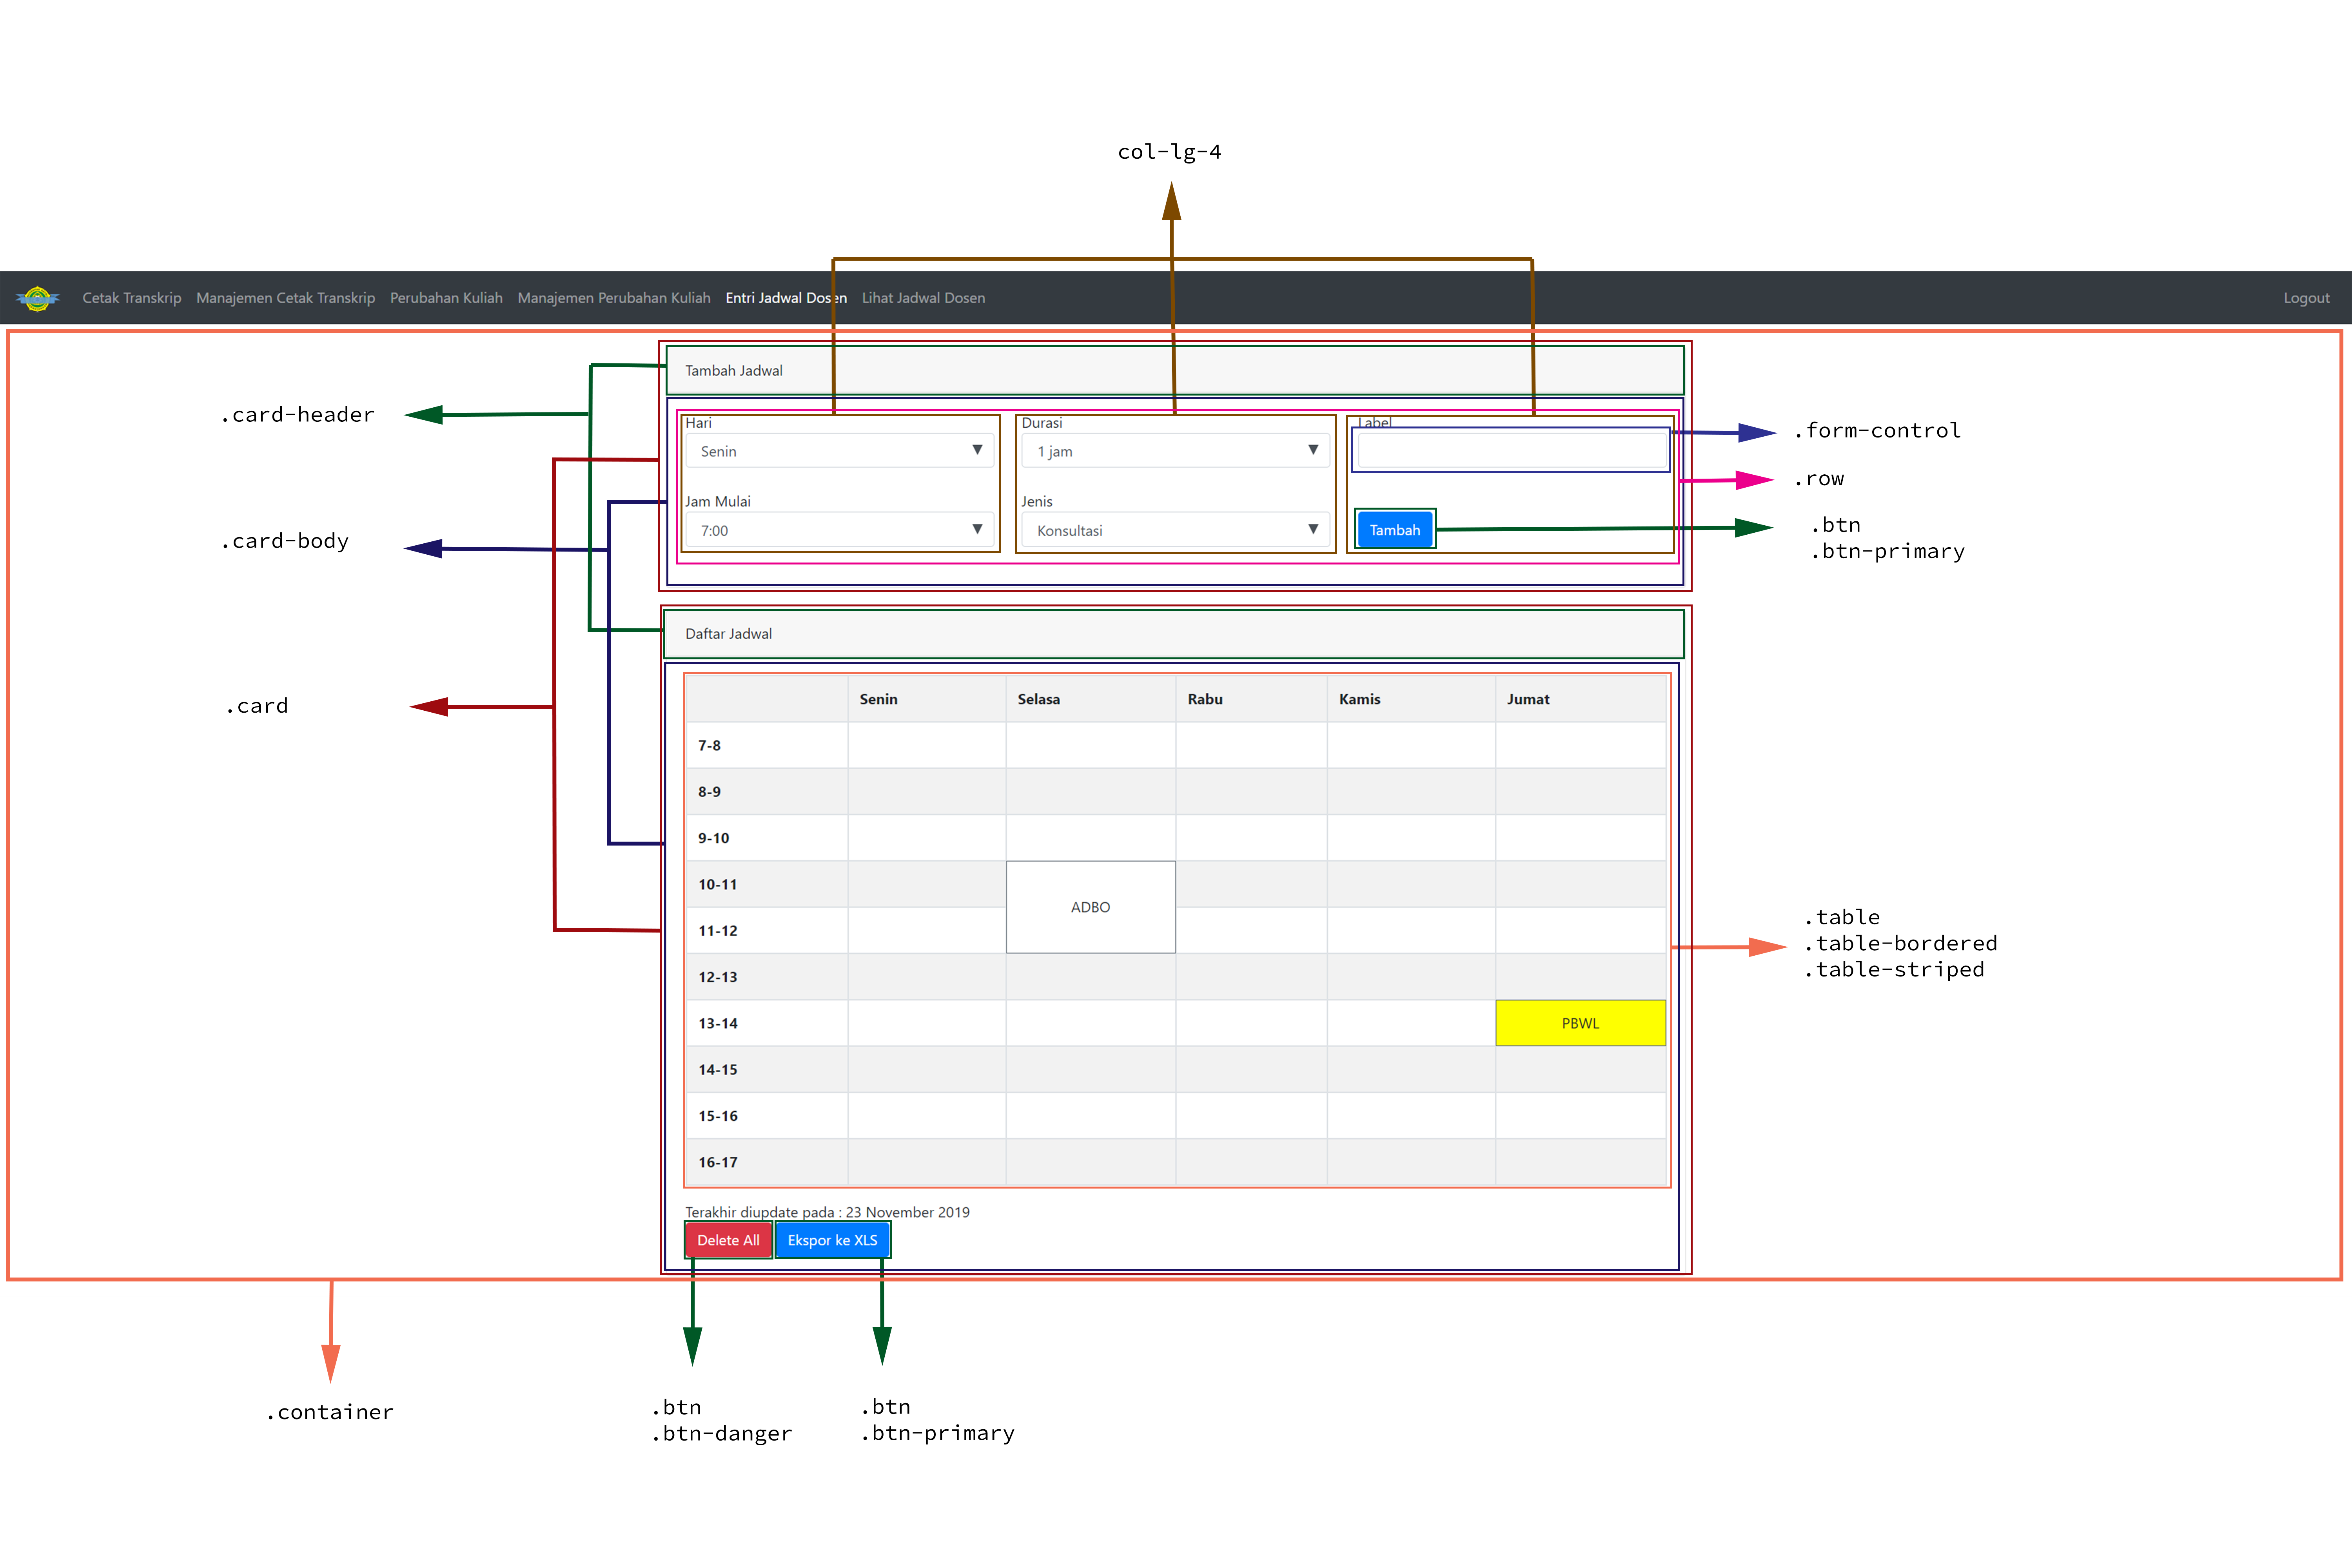
\includegraphics[width=\textwidth,height=\textheight,keepaspectratio]{bootstrap/konversi_tampilan_entri_jadwal_dosen.png}
	\caption{Konversi Halaman Entri Jadwal Dosen}
\end{figure}
\begin{lstlisting}[language=diff, caption=Kode untuk Halaman Entri Jadwal Dosen, label=Entri, basicstyle=\ttfamily, frame=single,
columns=fullflexible, keepspaces=true, breaklines=true]
--- C:\xampp\htdocs\BlueTape2\www\application\views\EntriJadwalDosen\main.php
+++ C:\xampp\htdocs\BlueTape\www\application\views\EntriJadwalDosen\main.php

@@ Implementasi Komponen Grid @@
+ <div class="container">
+    <div class="card">
+        <div class="card-header">
+            Tambah Jadwal
+        </div>
+        <div class="card-body">

- <div class="large-12 column callout">
-  <h5>Tambah Jadwal</h5>
-    <div class="large-4 columns">
+ <div class="col-lg-4">

@@ Implementasi Komponen Form @@
- <select name="hari"> 
+        <select class="form-control" name="hari">

- <select name="jam_mulai"> 
+        <select class="form-control" name="jam_mulai">

- <div class=" large-4 columns">
+ <div class="col-lg-4">

- <select name="durasi"> 
+    <select class="form-control" name="durasi">

- <select name="jenis_jadwal"> 
+    <select class="form-control" name="jenis_jadwal">

- <div class="large-4 columns">
-    Label <input type="text" name="label_jadwal"><br>
-    <input type="submit" class="button" value="Tambah">
-    </form>
+ <div class="col-lg-4">
+    Label <input class="form-control" type="text" name="label_jadwal"><br><br>
+    <input class="btn btn-primary" type="submit" value="Tambah">
+    </form><br>

@@ Implemetasi Komponen Card dan Tabel @@
-
- <div class="large-12 column callout">
-    <h5>Daftar Jadwal</h5>
- <div class="table-scroll" id="jadwal_table">
-	<table border=1 style="border-color:black ; border-collapse:separate">
+ <br>
+ <div class="card">
+ <div class="card-header">
+    Daftar Jadwal
+ </div>
+ <div class="card-body">
+    <div id="jadwal_table">
+        <table class="table table-bordered table-striped">

@@ Perubahan Style di jQuery @@
- <td style='width:10%'></td>
+ <th></th>

@@ Perubahan Style di jQuery @@
for ($i = 0; $i < 5; $i++) {
- echo "<td style='width:18%'> $namaHari[$i] </td>"; //Membuat Header Tabel yang berisi daftar hari
+ echo "<th> $namaHari[$i] </th>"; //Membuat Header Tabel yang berisi daftar hari

@@ Pemberian Border di jQuery @@

foreach ($dataJadwal as $dataHariIni) {
$colIdx = $dataHariIni->hari + 1;   // + 1 karena perbedaan selisih index tabel dan value hari di database 
$rowIdx = $dataHariIni->jam_mulai - 6;  // + 1 karena perbedaan selisih index tabel dan value jam_mulai di database 
+ $border = "border border-secondary align-middle";


@@ Implementasi jQuery untuk Tabel @@
$($cellLocation).css('background-color', '<?php echo $color; ?>');
$($cellLocation).attr('rowspan', <?php echo $dataHariIni->durasi ?>);
+ $($cellLocation).addClass('<?php echo $border; ?>');

@@ Implementasi jQuery untuk Modal @@
- $($menuName).foundation('open');
+ $($menuName).modal();

@@ Implementasi Komponen Form @@
- <a href="/EntriJadwalDosen/deleteAll/export/" class="alert button" onClick="return konfirmasi();">Delete All</a>
- <a href="/EntriJadwalDosen/export/" class="button">Ekspor ke XLS</a>
+ <a href="/EntriJadwalDosen/deleteAll/export/" class="btn btn-danger" onClick="return konfirmasi();">Delete All</a>
+ <a href="/EntriJadwalDosen/export/" class="btn btn-primary">Ekspor ke XLS</a>

@@ Implementasi Komponen Grid @@
- <div class="large-2 column ">
+ <div class="col-lg-2">


@@ Implementasi Komponen Button@@
- <input type="submit" id="deletebtn<?php echo $dataHariIni->id ?>" name="deletebtn<?php echo $dataHariIni->id ?>" class="alert button" value="Delete">
- </form><div>
+ <input class="btn btn-danger" type="submit" id="deletebtn<?php echo $dataHariIni->id ?>" name="deletebtn<?php echo $dataHariIni->id ?>" value="Delete">
+ </form>
\end{lstlisting}

\subsubsection{Modal}
\begin{figure} [H]
	\centering  
	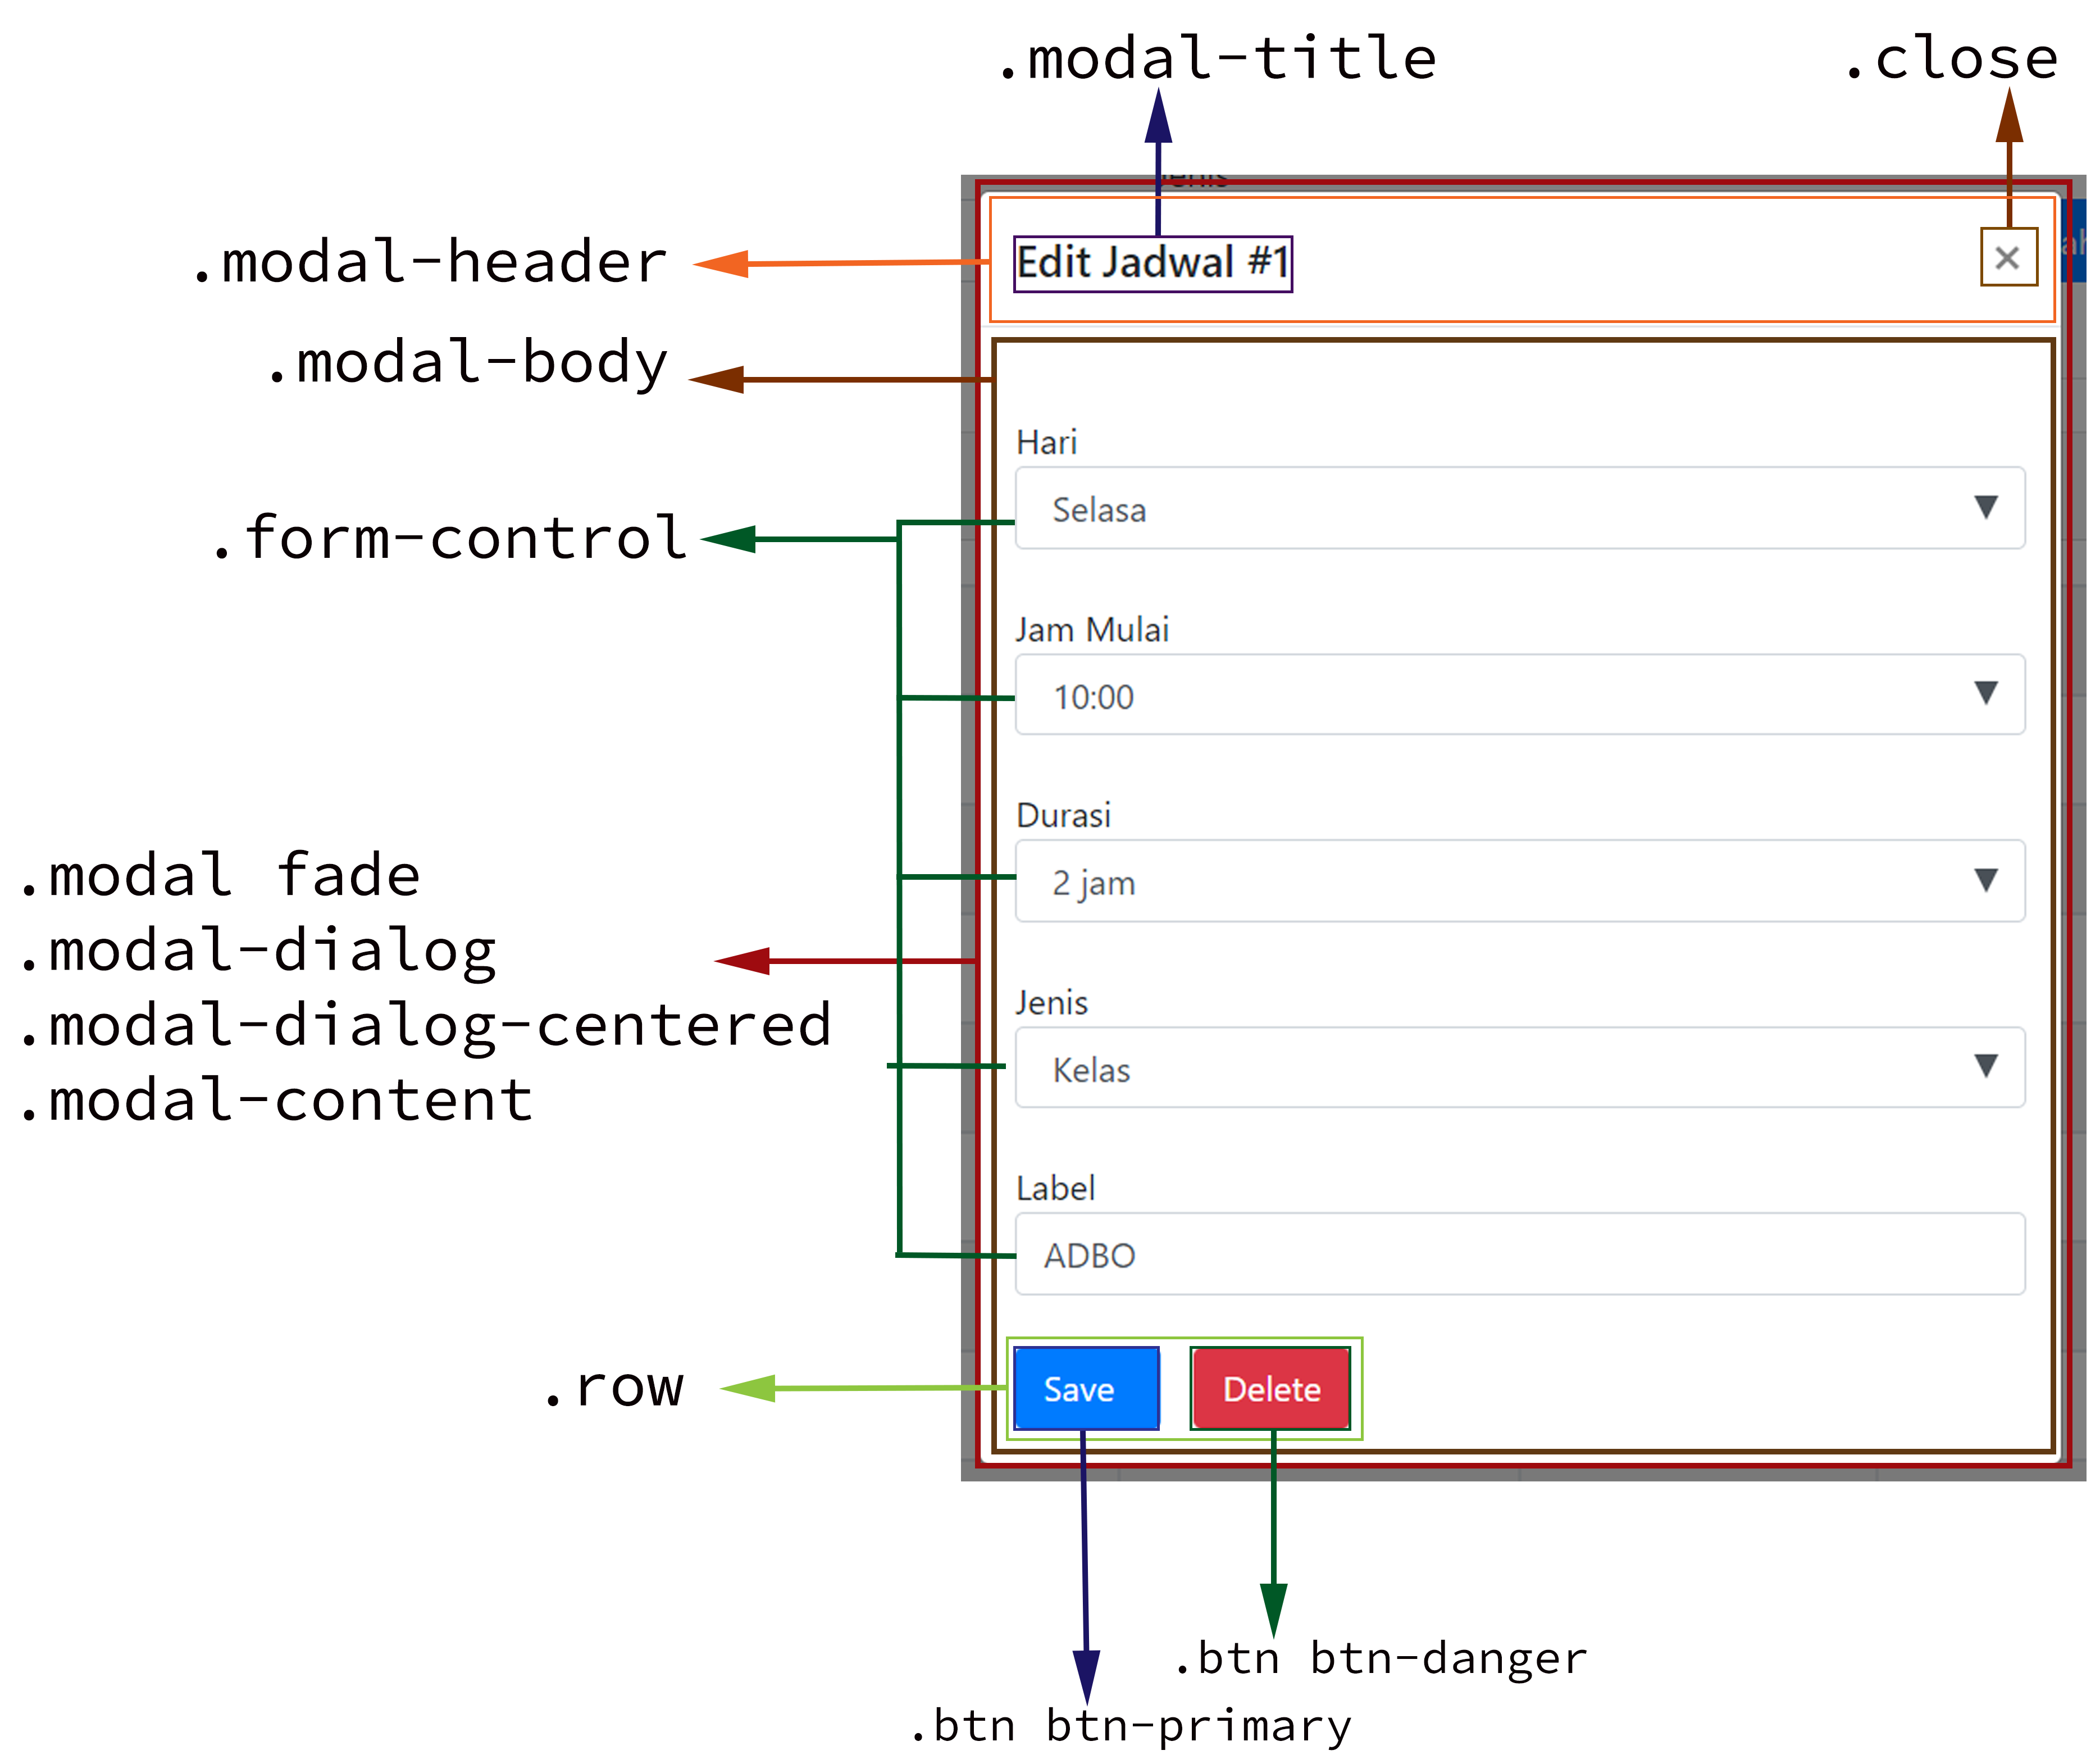
\includegraphics[width=\textwidth,height=\textheight,keepaspectratio]{bootstrap/konversi_modal_edit_jadwal_entri_jadwal_dosen.png}
	\caption{Modal Edit}
\end{figure}
\begin{lstlisting}[language=diff, label=Entri, basicstyle=\ttfamily, frame=single,
columns=fullflexible, keepspaces=true, breaklines=true]
@@ Implementasi Komponen Modal @@
- <div id="edit_menu<?php echo $dataHariIni->id ?>" class="reveal"  data-reveal >
- 		<button class="close-button" data-close aria-label="Close modal" type="button">
+ <div class="modal fade" id="edit_menu<?php echo $dataHariIni->id ?>" tabindex="-1" role="dialog" aria-hidden="true">
+  <div class="modal-dialog modal-dialog-centered" role="document">
+   <div class="modal-content">
+    <div class="modal-header">
+     <h5 class="modal-title" id="exampleModalLongTitle">Edit Jadwal #<?= $dataHariIni->id ?></h5>
+ 		<button type="button" class="close" data-dismiss="modal" aria-label="Close">

@@ Implementasi Komponen Form @@
- <select name="hari"> 
+ <select class="form-control" name="hari">

- <select name="jam_mulai"> 
+ <select class="form-control" name="jam_mulai">

- <select name="durasi"> 
+ <select class="form-control" name="durasi">

- <select name="jenis_jadwal"> 
+ <select class="form-control" name="jenis_jadwal">

- </select>
- Label <input type="text" name="label_jadwal" value="<?php echo $dataHariIni->label; ?>"><br> 
-   <div class="row large-4 column">
-    <div class="large-2 column">
-        <input type="submit" name="submitId<?php echo $dataHariIni->id ?>" class="button" value="Save  ">
-        </form>
+ </select><br>
+ Label
+ <input class="form-control" type="text" name="label_jadwal" value="<?php echo $dataHariIni->label; ?>"><br>
+   <div class="row">
+    <div class="col-lg-2">
+       <input class="btn btn-primary" type="submit" name="submitId<?php echo $dataHariIni->id ?>" class="button" value="Save  ">
\end{lstlisting}

\end{lstlisting}
\subsection{Halaman	Lihat Jadwal Dosen}
\begin{figure} [H]
	\centering  
	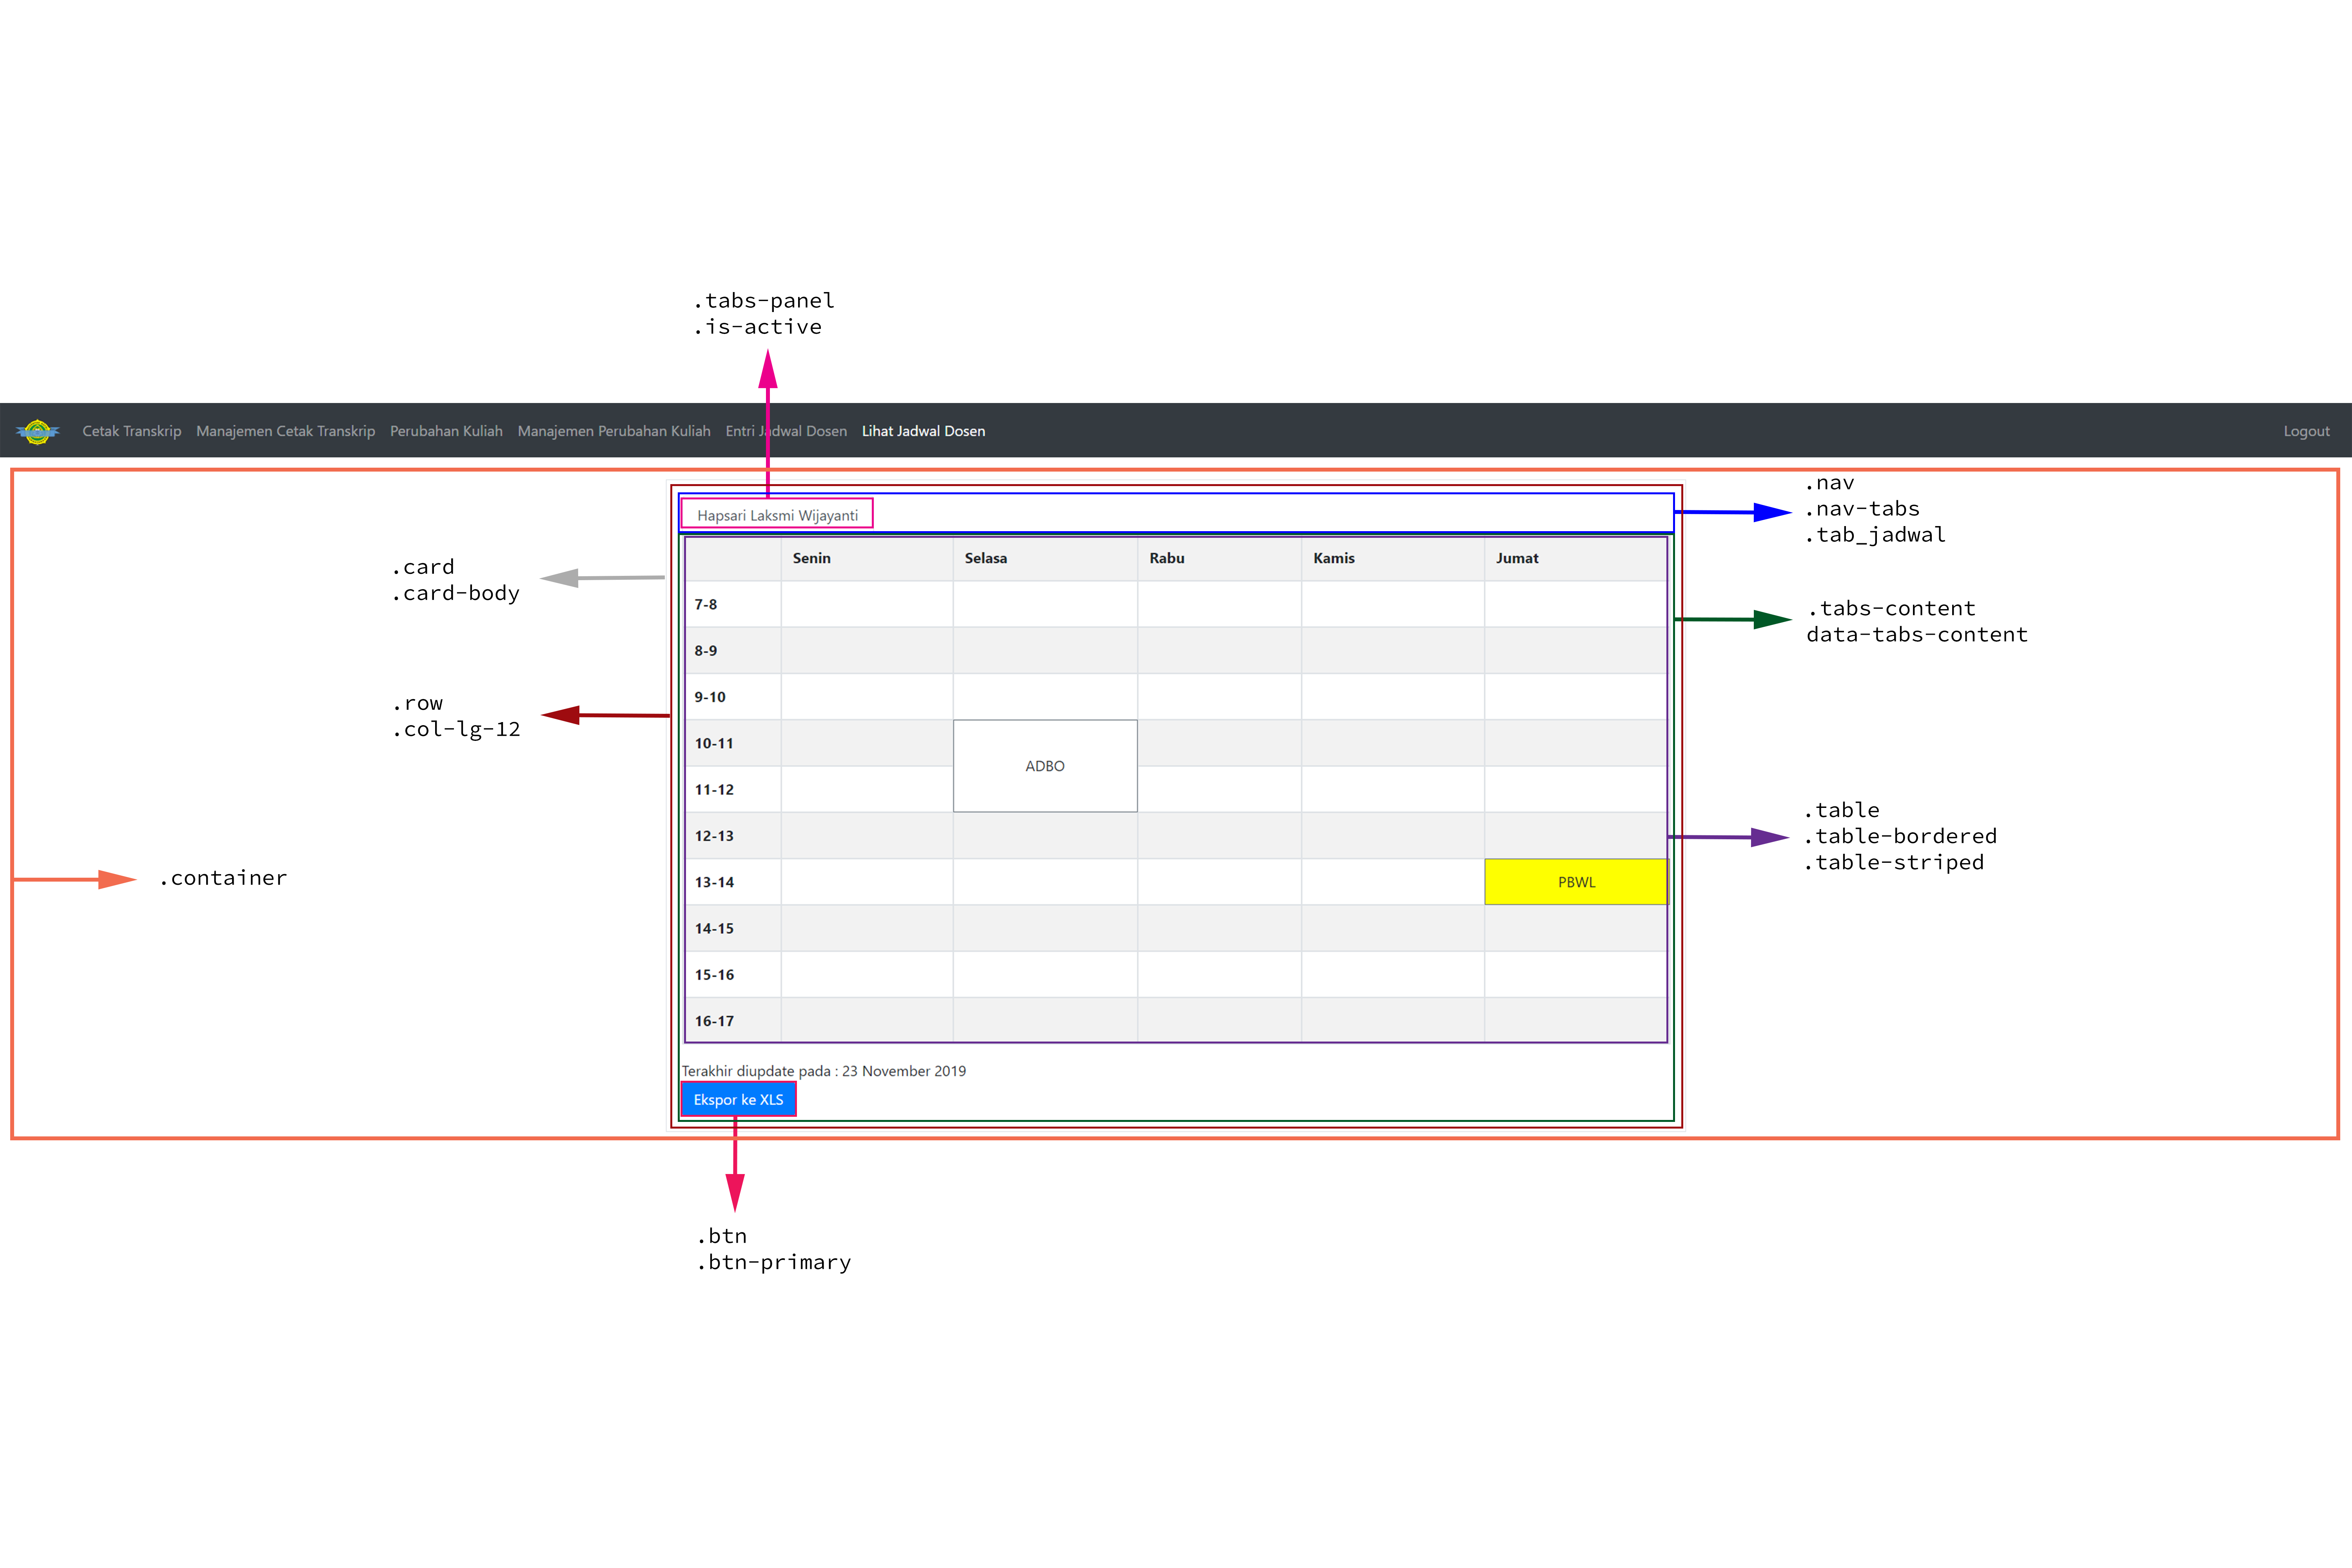
\includegraphics[width=\textwidth,height=\textheight,keepaspectratio]{bootstrap/konversi_lihat_jadwal_dosen.png}
	\caption{Konversi Halaman	Lihat Jadwal Dosen}
\end{figure}
\begin{lstlisting}[language=diff, caption=Kode untuk Halaman Lihat Jadwal Dosen, label=Entri, basicstyle=\ttfamily, frame=single,
columns=fullflexible, keepspaces=true, breaklines=true]
--- C:\xampp\htdocs\BlueTape2\www\application\views\LihatJadwalDosen\main.php
+++ C:\xampp\htdocs\BlueTape\www\application\views\LihatJadwalDosen\main.php

@@ Implementasi Komponen Grid dan Card @@
-
+ <div class="container">
+    <div class="card card-body">

@@ Implementasi Komponen Tabs @@
- <div class="large-12 column">
- <ul class="tabs" data-tabs id="tab_jadwal">
+ <div class="col-lg-12">
+	<ul class="nav nav-tabs" data-tabs id="tab_jadwal">

- <li class="tabs-title is-active"><a href="#hal<?php echo $idx; ?>" aria-selected="true"><?php foreach ($currRow as $data) {
+ <li class="nav-item"><a class="nav-link active" href="#hal<?php echo $idx; ?>" 

- <li class="tabs-title"><a a href="#hal<?php echo $idx; ?>"><?php foreach ($currRow as $data) {
+ <li class="nav-item"><a class="nav-link" href="#hal<?php echo $idx; ?>"><?php foreach ($currRow as $data) {

@@ Implementasi Styling Tabel Bergaris @@
- <div class="table-scroll" id="jadwal_table<?php echo $idx; ?>">
+ <div id="jadwal_table<?php echo $idx; ?>">

- <table id="tabel<?php echo $idx; ?>" border=1 style="border-color:black ; border-collapse:separate">
+ <table class="table table-bordered table-striped" id="tabel<?php echo $idx; ?>" >

@@ Perubahan Kode di jQuery @@
- echo "<td style='width:18%'>" . $namaHari[$i] . "</td>";
+ echo "<th>" . $namaHari[$i] . "</th>";

$colIdx = $dataHariIni->hari + 1;   // + 1 karena perbedaan selisih index tabel dan value hari di database 
$rowIdx = $dataHariIni->jam_mulai - 6;  // + 1 karena perbedaan selisih index tabel dan value jam_mulai di database 
+ $border = "border border-secondary align-middle";

$($cellLocation).css('background-color', '<?php echo $color; ?>');
$($cellLocation).attr('rowspan', <?php echo $dataHariIni->durasi ?>);
+ $($cellLocation).addClass('<?php echo $border; ?>');

@@ Implementasi Komponen Button @@
- <a href="/LihatJadwalDosen/export/" class="button">Ekspor ke XLS</a>
+ <a class="btn btn-primary" href="/LihatJadwalDosen/export/" class="button">Ekspor ke XLS</a>
\end{lstlisting}
